\chapter{Numerische Tests}
\label{cha:NumerischeTests}

In diesem Kapitel möchten wir die vorgestellten Verfahren verschiedenen numerischen Tests unterziehen. Dabei wollen wir hauptsächlich den Fehler der numerischen Lösung zur analytischen untersuchen, aber auch die Kondition der Kollokationsmatrizen, die Parameterwahl und die Laufzeit betrachten. Außerdem wollen wir die Verfahren mit der finiten Elemente Methode (\acs{FEM}) vergleichen. \glsunset{FEM}

Dafür betrachten wir die Poisson Gleichung auf zwei verschiedenen Gebieten und mit zwei verschiedenen rechten Seiten.
\begin{enumerate}
\item
Sei $\Omega := [-1,1] \times [-1,1] \subset \mathbb{R}^2$ und folgende \ac{PDE} gegeben:
\begin{align*}
- \Delta u &= 2\pi^2 \sin(\pi x)\sin(\pi y)&& (x,y) \in \Omega^\circ\\
u &= 0&& (x,y) \in \partial \Omega
\end{align*}
Sie hat die analytische Lösung 
\begin{align*}
u(x,y) = \sin(\pi x)\sin(\pi y),
\end{align*}
dargestellt in Abbildung \ref{fig:pde1sol}. Wir wählen als Gewichtsfunktion $w$ für $\Omega$ die Funktion aus Beispiel \ref{ex:Gewicht}:
\begin{align*}
w(x,y) = -x^2-y^2+2 - \sqrt{x^4 -2x^2 + y^4 -2y^2+2}.
\end{align*}
\begin{figure}[ht]
\centering
\resizebox {\columnwidth} {!} {
% This file was created by matlab2tikz.
%
%The latest updates can be retrieved from
%  http://www.mathworks.com/matlabcentral/fileexchange/22022-matlab2tikz-matlab2tikz
%where you can also make suggestions and rate matlab2tikz.
%
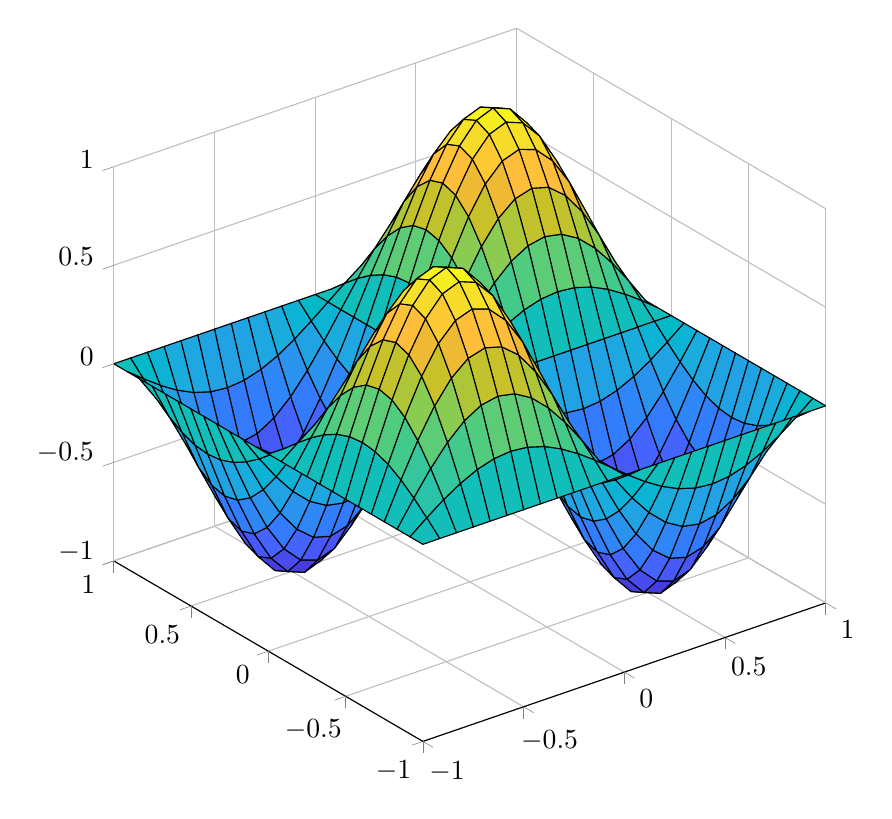
\begin{tikzpicture}

\begin{axis}[%
width=3.56in,
height=3.566in,
at={(0.597in,0.481in)},
scale only axis,
xmin=-1,
xmax=1,
tick align=outside,
ymin=-1,
ymax=1,
zmin=-1,
zmax=1,
view={-37.5}{30},
axis background/.style={fill=white},
axis x line*=bottom,
axis y line*=left,
axis z line*=left,
xmajorgrids,
ymajorgrids,
zmajorgrids,
legend style={at={(1.03,1)}, anchor=north west, legend cell align=left, align=left, draw=white!15!black}
]

\addplot3[%
surf,
shader=flat corner, draw=black, z buffer=sort, colormap={mymap}{[1pt] rgb(0pt)=(0.2422,0.1504,0.6603); rgb(1pt)=(0.25039,0.164995,0.707614); rgb(2pt)=(0.257771,0.181781,0.751138); rgb(3pt)=(0.264729,0.197757,0.795214); rgb(4pt)=(0.270648,0.214676,0.836371); rgb(5pt)=(0.275114,0.234238,0.870986); rgb(6pt)=(0.2783,0.255871,0.899071); rgb(7pt)=(0.280333,0.278233,0.9221); rgb(8pt)=(0.281338,0.300595,0.941376); rgb(9pt)=(0.281014,0.322757,0.957886); rgb(10pt)=(0.279467,0.344671,0.971676); rgb(11pt)=(0.275971,0.366681,0.982905); rgb(12pt)=(0.269914,0.3892,0.9906); rgb(13pt)=(0.260243,0.412329,0.995157); rgb(14pt)=(0.244033,0.435833,0.998833); rgb(15pt)=(0.220643,0.460257,0.997286); rgb(16pt)=(0.196333,0.484719,0.989152); rgb(17pt)=(0.183405,0.507371,0.979795); rgb(18pt)=(0.178643,0.528857,0.968157); rgb(19pt)=(0.176438,0.549905,0.952019); rgb(20pt)=(0.168743,0.570262,0.935871); rgb(21pt)=(0.154,0.5902,0.9218); rgb(22pt)=(0.146029,0.609119,0.907857); rgb(23pt)=(0.138024,0.627629,0.89729); rgb(24pt)=(0.124814,0.645929,0.888343); rgb(25pt)=(0.111252,0.6635,0.876314); rgb(26pt)=(0.0952095,0.679829,0.859781); rgb(27pt)=(0.0688714,0.694771,0.839357); rgb(28pt)=(0.0296667,0.708167,0.816333); rgb(29pt)=(0.00357143,0.720267,0.7917); rgb(30pt)=(0.00665714,0.731214,0.766014); rgb(31pt)=(0.0433286,0.741095,0.73941); rgb(32pt)=(0.0963952,0.75,0.712038); rgb(33pt)=(0.140771,0.7584,0.684157); rgb(34pt)=(0.1717,0.766962,0.655443); rgb(35pt)=(0.193767,0.775767,0.6251); rgb(36pt)=(0.216086,0.7843,0.5923); rgb(37pt)=(0.246957,0.791795,0.556743); rgb(38pt)=(0.290614,0.79729,0.518829); rgb(39pt)=(0.340643,0.8008,0.478857); rgb(40pt)=(0.3909,0.802871,0.435448); rgb(41pt)=(0.445629,0.802419,0.390919); rgb(42pt)=(0.5044,0.7993,0.348); rgb(43pt)=(0.561562,0.794233,0.304481); rgb(44pt)=(0.617395,0.787619,0.261238); rgb(45pt)=(0.671986,0.779271,0.2227); rgb(46pt)=(0.7242,0.769843,0.191029); rgb(47pt)=(0.773833,0.759805,0.16461); rgb(48pt)=(0.820314,0.749814,0.153529); rgb(49pt)=(0.863433,0.7406,0.159633); rgb(50pt)=(0.903543,0.733029,0.177414); rgb(51pt)=(0.939257,0.728786,0.209957); rgb(52pt)=(0.972757,0.729771,0.239443); rgb(53pt)=(0.995648,0.743371,0.237148); rgb(54pt)=(0.996986,0.765857,0.219943); rgb(55pt)=(0.995205,0.789252,0.202762); rgb(56pt)=(0.9892,0.813567,0.188533); rgb(57pt)=(0.978629,0.838629,0.176557); rgb(58pt)=(0.967648,0.8639,0.16429); rgb(59pt)=(0.96101,0.889019,0.153676); rgb(60pt)=(0.959671,0.913457,0.142257); rgb(61pt)=(0.962795,0.937338,0.12651); rgb(62pt)=(0.969114,0.960629,0.106362); rgb(63pt)=(0.9769,0.9839,0.0805)}, mesh/rows=25]
table[row sep=crcr, point meta=\thisrow{c}] {%
%
x	y	z	c\\
-1	-1	1.49975978266186e-32	1.49975978266186e-32\\
-0.916666666666667	-1	0	0\\
-0.833333333333333	-1	6.12323399573676e-17	6.12323399573676e-17\\
-0.75	-1	8.65956056235493e-17	8.65956056235493e-17\\
-0.666666666666667	-1	1.06057523872491e-16	1.06057523872491e-16\\
-0.583333333333333	-1	1.18291797137867e-16	1.18291797137867e-16\\
-0.5	-1	1.22464679914735e-16	1.22464679914735e-16\\
-0.416666666666667	-1	1.18291797137867e-16	1.18291797137867e-16\\
-0.333333333333333	-1	1.06057523872491e-16	1.06057523872491e-16\\
-0.25	-1	8.65956056235493e-17	8.65956056235493e-17\\
-0.166666666666667	-1	6.12323399573676e-17	6.12323399573676e-17\\
-0.0833333333333334	-1	3.16961915143177e-17	3.16961915143177e-17\\
0	-1	-0	-0\\
0.0833333333333333	-1	-3.16961915143176e-17	-3.16961915143176e-17\\
0.166666666666667	-1	-6.12323399573677e-17	-6.12323399573677e-17\\
0.25	-1	-8.65956056235493e-17	-8.65956056235493e-17\\
0.333333333333333	-1	-1.06057523872491e-16	-1.06057523872491e-16\\
0.416666666666667	-1	-1.18291797137867e-16	-1.18291797137867e-16\\
0.5	-1	-1.22464679914735e-16	-1.22464679914735e-16\\
0.583333333333333	-1	-1.18291797137867e-16	-1.18291797137867e-16\\
0.666666666666667	-1	-1.06057523872491e-16	-1.06057523872491e-16\\
0.75	-1	-8.65956056235493e-17	-8.65956056235493e-17\\
0.833333333333333	-1	-6.12323399573677e-17	-6.12323399573677e-17\\
0.916666666666667	-1	-3.16961915143176e-17	-3.16961915143176e-17\\
1	-1	-1.49975978266186e-32	-1.49975978266186e-32\\
-1	-0.916666666666667	3.16961915143177e-17	3.16961915143177e-17\\
-0.916666666666667	-0.916666666666667	0.0669872981077808	0.0669872981077808\\
-0.833333333333333	-0.916666666666667	0.12940952255126	0.12940952255126\\
-0.75	-0.916666666666667	0.18301270189222	0.18301270189222\\
-0.666666666666667	-0.916666666666667	0.224143868042014	0.224143868042014\\
-0.583333333333333	-0.916666666666667	0.25	0.25\\
-0.5	-0.916666666666667	0.258819045102521	0.258819045102521\\
-0.416666666666667	-0.916666666666667	0.25	0.25\\
-0.333333333333333	-0.916666666666667	0.224143868042014	0.224143868042014\\
-0.25	-0.916666666666667	0.183012701892219	0.183012701892219\\
-0.166666666666667	-0.916666666666667	0.12940952255126	0.12940952255126\\
-0.0833333333333334	-0.916666666666667	0.0669872981077808	0.0669872981077808\\
0	-0.916666666666667	-0	-0\\
0.0833333333333333	-0.916666666666667	-0.0669872981077807	-0.0669872981077807\\
0.166666666666667	-0.916666666666667	-0.129409522551261	-0.129409522551261\\
0.25	-0.916666666666667	-0.183012701892219	-0.183012701892219\\
0.333333333333333	-0.916666666666667	-0.224143868042014	-0.224143868042014\\
0.416666666666667	-0.916666666666667	-0.25	-0.25\\
0.5	-0.916666666666667	-0.258819045102521	-0.258819045102521\\
0.583333333333333	-0.916666666666667	-0.25	-0.25\\
0.666666666666667	-0.916666666666667	-0.224143868042014	-0.224143868042014\\
0.75	-0.916666666666667	-0.18301270189222	-0.18301270189222\\
0.833333333333333	-0.916666666666667	-0.129409522551261	-0.129409522551261\\
0.916666666666667	-0.916666666666667	-0.0669872981077807	-0.0669872981077807\\
1	-0.916666666666667	-3.16961915143177e-17	-3.16961915143177e-17\\
-1	-0.833333333333333	6.12323399573676e-17	6.12323399573676e-17\\
-0.916666666666667	-0.833333333333333	0.12940952255126	0.12940952255126\\
-0.833333333333333	-0.833333333333333	0.25	0.25\\
-0.75	-0.833333333333333	0.353553390593274	0.353553390593274\\
-0.666666666666667	-0.833333333333333	0.433012701892219	0.433012701892219\\
-0.583333333333333	-0.833333333333333	0.482962913144534	0.482962913144534\\
-0.5	-0.833333333333333	0.5	0.5\\
-0.416666666666667	-0.833333333333333	0.482962913144534	0.482962913144534\\
-0.333333333333333	-0.833333333333333	0.433012701892219	0.433012701892219\\
-0.25	-0.833333333333333	0.353553390593274	0.353553390593274\\
-0.166666666666667	-0.833333333333333	0.25	0.25\\
-0.0833333333333334	-0.833333333333333	0.12940952255126	0.12940952255126\\
0	-0.833333333333333	-0	-0\\
0.0833333333333333	-0.833333333333333	-0.12940952255126	-0.12940952255126\\
0.166666666666667	-0.833333333333333	-0.25	-0.25\\
0.25	-0.833333333333333	-0.353553390593274	-0.353553390593274\\
0.333333333333333	-0.833333333333333	-0.433012701892219	-0.433012701892219\\
0.416666666666667	-0.833333333333333	-0.482962913144534	-0.482962913144534\\
0.5	-0.833333333333333	-0.5	-0.5\\
0.583333333333333	-0.833333333333333	-0.482962913144534	-0.482962913144534\\
0.666666666666667	-0.833333333333333	-0.433012701892219	-0.433012701892219\\
0.75	-0.833333333333333	-0.353553390593274	-0.353553390593274\\
0.833333333333333	-0.833333333333333	-0.25	-0.25\\
0.916666666666667	-0.833333333333333	-0.12940952255126	-0.12940952255126\\
1	-0.833333333333333	-6.12323399573676e-17	-6.12323399573676e-17\\
-1	-0.75	8.65956056235493e-17	8.65956056235493e-17\\
-0.916666666666667	-0.75	0.18301270189222	0.18301270189222\\
-0.833333333333333	-0.75	0.353553390593274	0.353553390593274\\
-0.75	-0.75	0.5	0.5\\
-0.666666666666667	-0.75	0.612372435695795	0.612372435695795\\
-0.583333333333333	-0.75	0.68301270189222	0.68301270189222\\
-0.5	-0.75	0.707106781186548	0.707106781186548\\
-0.416666666666667	-0.75	0.683012701892219	0.683012701892219\\
-0.333333333333333	-0.75	0.612372435695795	0.612372435695795\\
-0.25	-0.75	0.5	0.5\\
-0.166666666666667	-0.75	0.353553390593274	0.353553390593274\\
-0.0833333333333334	-0.75	0.183012701892219	0.183012701892219\\
0	-0.75	-0	-0\\
0.0833333333333333	-0.75	-0.183012701892219	-0.183012701892219\\
0.166666666666667	-0.75	-0.353553390593274	-0.353553390593274\\
0.25	-0.75	-0.5	-0.5\\
0.333333333333333	-0.75	-0.612372435695794	-0.612372435695794\\
0.416666666666667	-0.75	-0.683012701892219	-0.683012701892219\\
0.5	-0.75	-0.707106781186548	-0.707106781186548\\
0.583333333333333	-0.75	-0.68301270189222	-0.68301270189222\\
0.666666666666667	-0.75	-0.612372435695795	-0.612372435695795\\
0.75	-0.75	-0.5	-0.5\\
0.833333333333333	-0.75	-0.353553390593274	-0.353553390593274\\
0.916666666666667	-0.75	-0.183012701892219	-0.183012701892219\\
1	-0.75	-8.65956056235493e-17	-8.65956056235493e-17\\
-1	-0.666666666666667	1.06057523872491e-16	1.06057523872491e-16\\
-0.916666666666667	-0.666666666666667	0.224143868042014	0.224143868042014\\
-0.833333333333333	-0.666666666666667	0.433012701892219	0.433012701892219\\
-0.75	-0.666666666666667	0.612372435695795	0.612372435695795\\
-0.666666666666667	-0.666666666666667	0.75	0.75\\
-0.583333333333333	-0.666666666666667	0.836516303737808	0.836516303737808\\
-0.5	-0.666666666666667	0.866025403784439	0.866025403784439\\
-0.416666666666667	-0.666666666666667	0.836516303737808	0.836516303737808\\
-0.333333333333333	-0.666666666666667	0.75	0.75\\
-0.25	-0.666666666666667	0.612372435695794	0.612372435695794\\
-0.166666666666667	-0.666666666666667	0.433012701892219	0.433012701892219\\
-0.0833333333333334	-0.666666666666667	0.224143868042013	0.224143868042013\\
0	-0.666666666666667	-0	-0\\
0.0833333333333333	-0.666666666666667	-0.224143868042013	-0.224143868042013\\
0.166666666666667	-0.666666666666667	-0.433012701892219	-0.433012701892219\\
0.25	-0.666666666666667	-0.612372435695794	-0.612372435695794\\
0.333333333333333	-0.666666666666667	-0.75	-0.75\\
0.416666666666667	-0.666666666666667	-0.836516303737808	-0.836516303737808\\
0.5	-0.666666666666667	-0.866025403784439	-0.866025403784439\\
0.583333333333333	-0.666666666666667	-0.836516303737808	-0.836516303737808\\
0.666666666666667	-0.666666666666667	-0.75	-0.75\\
0.75	-0.666666666666667	-0.612372435695795	-0.612372435695795\\
0.833333333333333	-0.666666666666667	-0.43301270189222	-0.43301270189222\\
0.916666666666667	-0.666666666666667	-0.224143868042013	-0.224143868042013\\
1	-0.666666666666667	-1.06057523872491e-16	-1.06057523872491e-16\\
-1	-0.583333333333333	1.18291797137867e-16	1.18291797137867e-16\\
-0.916666666666667	-0.583333333333333	0.25	0.25\\
-0.833333333333333	-0.583333333333333	0.482962913144534	0.482962913144534\\
-0.75	-0.583333333333333	0.68301270189222	0.68301270189222\\
-0.666666666666667	-0.583333333333333	0.836516303737808	0.836516303737808\\
-0.583333333333333	-0.583333333333333	0.93301270189222	0.93301270189222\\
-0.5	-0.583333333333333	0.965925826289068	0.965925826289068\\
-0.416666666666667	-0.583333333333333	0.933012701892219	0.933012701892219\\
-0.333333333333333	-0.583333333333333	0.836516303737808	0.836516303737808\\
-0.25	-0.583333333333333	0.683012701892219	0.683012701892219\\
-0.166666666666667	-0.583333333333333	0.482962913144534	0.482962913144534\\
-0.0833333333333334	-0.583333333333333	0.25	0.25\\
0	-0.583333333333333	-0	-0\\
0.0833333333333333	-0.583333333333333	-0.25	-0.25\\
0.166666666666667	-0.583333333333333	-0.482962913144534	-0.482962913144534\\
0.25	-0.583333333333333	-0.683012701892219	-0.683012701892219\\
0.333333333333333	-0.583333333333333	-0.836516303737808	-0.836516303737808\\
0.416666666666667	-0.583333333333333	-0.93301270189222	-0.93301270189222\\
0.5	-0.583333333333333	-0.965925826289068	-0.965925826289068\\
0.583333333333333	-0.583333333333333	-0.93301270189222	-0.93301270189222\\
0.666666666666667	-0.583333333333333	-0.836516303737808	-0.836516303737808\\
0.75	-0.583333333333333	-0.68301270189222	-0.68301270189222\\
0.833333333333333	-0.583333333333333	-0.482962913144535	-0.482962913144535\\
0.916666666666667	-0.583333333333333	-0.25	-0.25\\
1	-0.583333333333333	-1.18291797137867e-16	-1.18291797137867e-16\\
-1	-0.5	1.22464679914735e-16	1.22464679914735e-16\\
-0.916666666666667	-0.5	0.258819045102521	0.258819045102521\\
-0.833333333333333	-0.5	0.5	0.5\\
-0.75	-0.5	0.707106781186548	0.707106781186548\\
-0.666666666666667	-0.5	0.866025403784439	0.866025403784439\\
-0.583333333333333	-0.5	0.965925826289068	0.965925826289068\\
-0.5	-0.5	1	1\\
-0.416666666666667	-0.5	0.965925826289068	0.965925826289068\\
-0.333333333333333	-0.5	0.866025403784439	0.866025403784439\\
-0.25	-0.5	0.707106781186547	0.707106781186547\\
-0.166666666666667	-0.5	0.5	0.5\\
-0.0833333333333334	-0.5	0.258819045102521	0.258819045102521\\
0	-0.5	-0	-0\\
0.0833333333333333	-0.5	-0.258819045102521	-0.258819045102521\\
0.166666666666667	-0.5	-0.5	-0.5\\
0.25	-0.5	-0.707106781186547	-0.707106781186547\\
0.333333333333333	-0.5	-0.866025403784438	-0.866025403784438\\
0.416666666666667	-0.5	-0.965925826289068	-0.965925826289068\\
0.5	-0.5	-1	-1\\
0.583333333333333	-0.5	-0.965925826289068	-0.965925826289068\\
0.666666666666667	-0.5	-0.866025403784439	-0.866025403784439\\
0.75	-0.5	-0.707106781186548	-0.707106781186548\\
0.833333333333333	-0.5	-0.5	-0.5\\
0.916666666666667	-0.5	-0.258819045102521	-0.258819045102521\\
1	-0.5	-1.22464679914735e-16	-1.22464679914735e-16\\
-1	-0.416666666666667	1.18291797137867e-16	1.18291797137867e-16\\
-0.916666666666667	-0.416666666666667	0.25	0.25\\
-0.833333333333333	-0.416666666666667	0.482962913144534	0.482962913144534\\
-0.75	-0.416666666666667	0.683012701892219	0.683012701892219\\
-0.666666666666667	-0.416666666666667	0.836516303737808	0.836516303737808\\
-0.583333333333333	-0.416666666666667	0.933012701892219	0.933012701892219\\
-0.5	-0.416666666666667	0.965925826289068	0.965925826289068\\
-0.416666666666667	-0.416666666666667	0.933012701892219	0.933012701892219\\
-0.333333333333333	-0.416666666666667	0.836516303737808	0.836516303737808\\
-0.25	-0.416666666666667	0.683012701892219	0.683012701892219\\
-0.166666666666667	-0.416666666666667	0.482962913144534	0.482962913144534\\
-0.0833333333333334	-0.416666666666667	0.25	0.25\\
0	-0.416666666666667	-0	-0\\
0.0833333333333333	-0.416666666666667	-0.25	-0.25\\
0.166666666666667	-0.416666666666667	-0.482962913144534	-0.482962913144534\\
0.25	-0.416666666666667	-0.683012701892219	-0.683012701892219\\
0.333333333333333	-0.416666666666667	-0.836516303737808	-0.836516303737808\\
0.416666666666667	-0.416666666666667	-0.933012701892219	-0.933012701892219\\
0.5	-0.416666666666667	-0.965925826289068	-0.965925826289068\\
0.583333333333333	-0.416666666666667	-0.933012701892219	-0.933012701892219\\
0.666666666666667	-0.416666666666667	-0.836516303737808	-0.836516303737808\\
0.75	-0.416666666666667	-0.683012701892219	-0.683012701892219\\
0.833333333333333	-0.416666666666667	-0.482962913144534	-0.482962913144534\\
0.916666666666667	-0.416666666666667	-0.25	-0.25\\
1	-0.416666666666667	-1.18291797137867e-16	-1.18291797137867e-16\\
-1	-0.333333333333333	1.06057523872491e-16	1.06057523872491e-16\\
-0.916666666666667	-0.333333333333333	0.224143868042014	0.224143868042014\\
-0.833333333333333	-0.333333333333333	0.433012701892219	0.433012701892219\\
-0.75	-0.333333333333333	0.612372435695795	0.612372435695795\\
-0.666666666666667	-0.333333333333333	0.75	0.75\\
-0.583333333333333	-0.333333333333333	0.836516303737808	0.836516303737808\\
-0.5	-0.333333333333333	0.866025403784439	0.866025403784439\\
-0.416666666666667	-0.333333333333333	0.836516303737808	0.836516303737808\\
-0.333333333333333	-0.333333333333333	0.75	0.75\\
-0.25	-0.333333333333333	0.612372435695794	0.612372435695794\\
-0.166666666666667	-0.333333333333333	0.433012701892219	0.433012701892219\\
-0.0833333333333334	-0.333333333333333	0.224143868042013	0.224143868042013\\
0	-0.333333333333333	-0	-0\\
0.0833333333333333	-0.333333333333333	-0.224143868042013	-0.224143868042013\\
0.166666666666667	-0.333333333333333	-0.433012701892219	-0.433012701892219\\
0.25	-0.333333333333333	-0.612372435695794	-0.612372435695794\\
0.333333333333333	-0.333333333333333	-0.75	-0.75\\
0.416666666666667	-0.333333333333333	-0.836516303737808	-0.836516303737808\\
0.5	-0.333333333333333	-0.866025403784439	-0.866025403784439\\
0.583333333333333	-0.333333333333333	-0.836516303737808	-0.836516303737808\\
0.666666666666667	-0.333333333333333	-0.75	-0.75\\
0.75	-0.333333333333333	-0.612372435695795	-0.612372435695795\\
0.833333333333333	-0.333333333333333	-0.43301270189222	-0.43301270189222\\
0.916666666666667	-0.333333333333333	-0.224143868042013	-0.224143868042013\\
1	-0.333333333333333	-1.06057523872491e-16	-1.06057523872491e-16\\
-1	-0.25	8.65956056235493e-17	8.65956056235493e-17\\
-0.916666666666667	-0.25	0.183012701892219	0.183012701892219\\
-0.833333333333333	-0.25	0.353553390593274	0.353553390593274\\
-0.75	-0.25	0.5	0.5\\
-0.666666666666667	-0.25	0.612372435695794	0.612372435695794\\
-0.583333333333333	-0.25	0.683012701892219	0.683012701892219\\
-0.5	-0.25	0.707106781186547	0.707106781186547\\
-0.416666666666667	-0.25	0.683012701892219	0.683012701892219\\
-0.333333333333333	-0.25	0.612372435695794	0.612372435695794\\
-0.25	-0.25	0.5	0.5\\
-0.166666666666667	-0.25	0.353553390593274	0.353553390593274\\
-0.0833333333333334	-0.25	0.183012701892219	0.183012701892219\\
0	-0.25	-0	-0\\
0.0833333333333333	-0.25	-0.183012701892219	-0.183012701892219\\
0.166666666666667	-0.25	-0.353553390593274	-0.353553390593274\\
0.25	-0.25	-0.5	-0.5\\
0.333333333333333	-0.25	-0.612372435695794	-0.612372435695794\\
0.416666666666667	-0.25	-0.683012701892219	-0.683012701892219\\
0.5	-0.25	-0.707106781186547	-0.707106781186547\\
0.583333333333333	-0.25	-0.683012701892219	-0.683012701892219\\
0.666666666666667	-0.25	-0.612372435695794	-0.612372435695794\\
0.75	-0.25	-0.5	-0.5\\
0.833333333333333	-0.25	-0.353553390593274	-0.353553390593274\\
0.916666666666667	-0.25	-0.183012701892219	-0.183012701892219\\
1	-0.25	-8.65956056235493e-17	-8.65956056235493e-17\\
-1	-0.166666666666667	6.12323399573676e-17	6.12323399573676e-17\\
-0.916666666666667	-0.166666666666667	0.12940952255126	0.12940952255126\\
-0.833333333333333	-0.166666666666667	0.25	0.25\\
-0.75	-0.166666666666667	0.353553390593274	0.353553390593274\\
-0.666666666666667	-0.166666666666667	0.433012701892219	0.433012701892219\\
-0.583333333333333	-0.166666666666667	0.482962913144534	0.482962913144534\\
-0.5	-0.166666666666667	0.5	0.5\\
-0.416666666666667	-0.166666666666667	0.482962913144534	0.482962913144534\\
-0.333333333333333	-0.166666666666667	0.433012701892219	0.433012701892219\\
-0.25	-0.166666666666667	0.353553390593274	0.353553390593274\\
-0.166666666666667	-0.166666666666667	0.25	0.25\\
-0.0833333333333334	-0.166666666666667	0.12940952255126	0.12940952255126\\
0	-0.166666666666667	-0	-0\\
0.0833333333333333	-0.166666666666667	-0.12940952255126	-0.12940952255126\\
0.166666666666667	-0.166666666666667	-0.25	-0.25\\
0.25	-0.166666666666667	-0.353553390593274	-0.353553390593274\\
0.333333333333333	-0.166666666666667	-0.433012701892219	-0.433012701892219\\
0.416666666666667	-0.166666666666667	-0.482962913144534	-0.482962913144534\\
0.5	-0.166666666666667	-0.5	-0.5\\
0.583333333333333	-0.166666666666667	-0.482962913144534	-0.482962913144534\\
0.666666666666667	-0.166666666666667	-0.433012701892219	-0.433012701892219\\
0.75	-0.166666666666667	-0.353553390593274	-0.353553390593274\\
0.833333333333333	-0.166666666666667	-0.25	-0.25\\
0.916666666666667	-0.166666666666667	-0.12940952255126	-0.12940952255126\\
1	-0.166666666666667	-6.12323399573676e-17	-6.12323399573676e-17\\
-1	-0.0833333333333334	3.16961915143177e-17	3.16961915143177e-17\\
-0.916666666666667	-0.0833333333333334	0.0669872981077808	0.0669872981077808\\
-0.833333333333333	-0.0833333333333334	0.12940952255126	0.12940952255126\\
-0.75	-0.0833333333333334	0.183012701892219	0.183012701892219\\
-0.666666666666667	-0.0833333333333334	0.224143868042013	0.224143868042013\\
-0.583333333333333	-0.0833333333333334	0.25	0.25\\
-0.5	-0.0833333333333334	0.258819045102521	0.258819045102521\\
-0.416666666666667	-0.0833333333333334	0.25	0.25\\
-0.333333333333333	-0.0833333333333334	0.224143868042013	0.224143868042013\\
-0.25	-0.0833333333333334	0.183012701892219	0.183012701892219\\
-0.166666666666667	-0.0833333333333334	0.12940952255126	0.12940952255126\\
-0.0833333333333334	-0.0833333333333334	0.0669872981077807	0.0669872981077807\\
0	-0.0833333333333334	-0	-0\\
0.0833333333333333	-0.0833333333333334	-0.0669872981077806	-0.0669872981077806\\
0.166666666666667	-0.0833333333333334	-0.12940952255126	-0.12940952255126\\
0.25	-0.0833333333333334	-0.183012701892219	-0.183012701892219\\
0.333333333333333	-0.0833333333333334	-0.224143868042013	-0.224143868042013\\
0.416666666666667	-0.0833333333333334	-0.25	-0.25\\
0.5	-0.0833333333333334	-0.258819045102521	-0.258819045102521\\
0.583333333333333	-0.0833333333333334	-0.25	-0.25\\
0.666666666666667	-0.0833333333333334	-0.224143868042013	-0.224143868042013\\
0.75	-0.0833333333333334	-0.183012701892219	-0.183012701892219\\
0.833333333333333	-0.0833333333333334	-0.129409522551261	-0.129409522551261\\
0.916666666666667	-0.0833333333333334	-0.0669872981077806	-0.0669872981077806\\
1	-0.0833333333333334	-3.16961915143177e-17	-3.16961915143177e-17\\
-1	0	-0	-0\\
-0.916666666666667	0	-0	-0\\
-0.833333333333333	0	-0	-0\\
-0.75	0	-0	-0\\
-0.666666666666667	0	-0	-0\\
-0.583333333333333	0	-0	-0\\
-0.5	0	-0	-0\\
-0.416666666666667	0	-0	-0\\
-0.333333333333333	0	-0	-0\\
-0.25	0	-0	-0\\
-0.166666666666667	0	-0	-0\\
-0.0833333333333334	0	-0	-0\\
0	0	0	0\\
0.0833333333333333	0	0	0\\
0.166666666666667	0	0	0\\
0.25	0	0	0\\
0.333333333333333	0	0	0\\
0.416666666666667	0	0	0\\
0.5	0	0	0\\
0.583333333333333	0	0	0\\
0.666666666666667	0	0	0\\
0.75	0	0	0\\
0.833333333333333	0	0	0\\
0.916666666666667	0	0	0\\
1	0	0	0\\
-1	0.0833333333333333	-3.16961915143176e-17	-3.16961915143176e-17\\
-0.916666666666667	0.0833333333333333	-0.0669872981077807	-0.0669872981077807\\
-0.833333333333333	0.0833333333333333	-0.12940952255126	-0.12940952255126\\
-0.75	0.0833333333333333	-0.183012701892219	-0.183012701892219\\
-0.666666666666667	0.0833333333333333	-0.224143868042013	-0.224143868042013\\
-0.583333333333333	0.0833333333333333	-0.25	-0.25\\
-0.5	0.0833333333333333	-0.258819045102521	-0.258819045102521\\
-0.416666666666667	0.0833333333333333	-0.25	-0.25\\
-0.333333333333333	0.0833333333333333	-0.224143868042013	-0.224143868042013\\
-0.25	0.0833333333333333	-0.183012701892219	-0.183012701892219\\
-0.166666666666667	0.0833333333333333	-0.12940952255126	-0.12940952255126\\
-0.0833333333333334	0.0833333333333333	-0.0669872981077806	-0.0669872981077806\\
0	0.0833333333333333	0	0\\
0.0833333333333333	0.0833333333333333	0.0669872981077805	0.0669872981077805\\
0.166666666666667	0.0833333333333333	0.12940952255126	0.12940952255126\\
0.25	0.0833333333333333	0.183012701892219	0.183012701892219\\
0.333333333333333	0.0833333333333333	0.224143868042013	0.224143868042013\\
0.416666666666667	0.0833333333333333	0.25	0.25\\
0.5	0.0833333333333333	0.258819045102521	0.258819045102521\\
0.583333333333333	0.0833333333333333	0.25	0.25\\
0.666666666666667	0.0833333333333333	0.224143868042013	0.224143868042013\\
0.75	0.0833333333333333	0.183012701892219	0.183012701892219\\
0.833333333333333	0.0833333333333333	0.12940952255126	0.12940952255126\\
0.916666666666667	0.0833333333333333	0.0669872981077806	0.0669872981077806\\
1	0.0833333333333333	3.16961915143176e-17	3.16961915143176e-17\\
-1	0.166666666666667	-6.12323399573677e-17	-6.12323399573677e-17\\
-0.916666666666667	0.166666666666667	-0.129409522551261	-0.129409522551261\\
-0.833333333333333	0.166666666666667	-0.25	-0.25\\
-0.75	0.166666666666667	-0.353553390593274	-0.353553390593274\\
-0.666666666666667	0.166666666666667	-0.433012701892219	-0.433012701892219\\
-0.583333333333333	0.166666666666667	-0.482962913144534	-0.482962913144534\\
-0.5	0.166666666666667	-0.5	-0.5\\
-0.416666666666667	0.166666666666667	-0.482962913144534	-0.482962913144534\\
-0.333333333333333	0.166666666666667	-0.433012701892219	-0.433012701892219\\
-0.25	0.166666666666667	-0.353553390593274	-0.353553390593274\\
-0.166666666666667	0.166666666666667	-0.25	-0.25\\
-0.0833333333333334	0.166666666666667	-0.12940952255126	-0.12940952255126\\
0	0.166666666666667	0	0\\
0.0833333333333333	0.166666666666667	0.12940952255126	0.12940952255126\\
0.166666666666667	0.166666666666667	0.25	0.25\\
0.25	0.166666666666667	0.353553390593274	0.353553390593274\\
0.333333333333333	0.166666666666667	0.433012701892219	0.433012701892219\\
0.416666666666667	0.166666666666667	0.482962913144534	0.482962913144534\\
0.5	0.166666666666667	0.5	0.5\\
0.583333333333333	0.166666666666667	0.482962913144534	0.482962913144534\\
0.666666666666667	0.166666666666667	0.433012701892219	0.433012701892219\\
0.75	0.166666666666667	0.353553390593274	0.353553390593274\\
0.833333333333333	0.166666666666667	0.25	0.25\\
0.916666666666667	0.166666666666667	0.12940952255126	0.12940952255126\\
1	0.166666666666667	6.12323399573677e-17	6.12323399573677e-17\\
-1	0.25	-8.65956056235493e-17	-8.65956056235493e-17\\
-0.916666666666667	0.25	-0.183012701892219	-0.183012701892219\\
-0.833333333333333	0.25	-0.353553390593274	-0.353553390593274\\
-0.75	0.25	-0.5	-0.5\\
-0.666666666666667	0.25	-0.612372435695794	-0.612372435695794\\
-0.583333333333333	0.25	-0.683012701892219	-0.683012701892219\\
-0.5	0.25	-0.707106781186547	-0.707106781186547\\
-0.416666666666667	0.25	-0.683012701892219	-0.683012701892219\\
-0.333333333333333	0.25	-0.612372435695794	-0.612372435695794\\
-0.25	0.25	-0.5	-0.5\\
-0.166666666666667	0.25	-0.353553390593274	-0.353553390593274\\
-0.0833333333333334	0.25	-0.183012701892219	-0.183012701892219\\
0	0.25	0	0\\
0.0833333333333333	0.25	0.183012701892219	0.183012701892219\\
0.166666666666667	0.25	0.353553390593274	0.353553390593274\\
0.25	0.25	0.5	0.5\\
0.333333333333333	0.25	0.612372435695794	0.612372435695794\\
0.416666666666667	0.25	0.683012701892219	0.683012701892219\\
0.5	0.25	0.707106781186547	0.707106781186547\\
0.583333333333333	0.25	0.683012701892219	0.683012701892219\\
0.666666666666667	0.25	0.612372435695794	0.612372435695794\\
0.75	0.25	0.5	0.5\\
0.833333333333333	0.25	0.353553390593274	0.353553390593274\\
0.916666666666667	0.25	0.183012701892219	0.183012701892219\\
1	0.25	8.65956056235493e-17	8.65956056235493e-17\\
-1	0.333333333333333	-1.06057523872491e-16	-1.06057523872491e-16\\
-0.916666666666667	0.333333333333333	-0.224143868042014	-0.224143868042014\\
-0.833333333333333	0.333333333333333	-0.433012701892219	-0.433012701892219\\
-0.75	0.333333333333333	-0.612372435695794	-0.612372435695794\\
-0.666666666666667	0.333333333333333	-0.75	-0.75\\
-0.583333333333333	0.333333333333333	-0.836516303737808	-0.836516303737808\\
-0.5	0.333333333333333	-0.866025403784438	-0.866025403784438\\
-0.416666666666667	0.333333333333333	-0.836516303737808	-0.836516303737808\\
-0.333333333333333	0.333333333333333	-0.75	-0.75\\
-0.25	0.333333333333333	-0.612372435695794	-0.612372435695794\\
-0.166666666666667	0.333333333333333	-0.433012701892219	-0.433012701892219\\
-0.0833333333333334	0.333333333333333	-0.224143868042013	-0.224143868042013\\
0	0.333333333333333	0	0\\
0.0833333333333333	0.333333333333333	0.224143868042013	0.224143868042013\\
0.166666666666667	0.333333333333333	0.433012701892219	0.433012701892219\\
0.25	0.333333333333333	0.612372435695794	0.612372435695794\\
0.333333333333333	0.333333333333333	0.75	0.75\\
0.416666666666667	0.333333333333333	0.836516303737808	0.836516303737808\\
0.5	0.333333333333333	0.866025403784438	0.866025403784438\\
0.583333333333333	0.333333333333333	0.836516303737808	0.836516303737808\\
0.666666666666667	0.333333333333333	0.75	0.75\\
0.75	0.333333333333333	0.612372435695794	0.612372435695794\\
0.833333333333333	0.333333333333333	0.43301270189222	0.43301270189222\\
0.916666666666667	0.333333333333333	0.224143868042013	0.224143868042013\\
1	0.333333333333333	1.06057523872491e-16	1.06057523872491e-16\\
-1	0.416666666666667	-1.18291797137867e-16	-1.18291797137867e-16\\
-0.916666666666667	0.416666666666667	-0.25	-0.25\\
-0.833333333333333	0.416666666666667	-0.482962913144534	-0.482962913144534\\
-0.75	0.416666666666667	-0.683012701892219	-0.683012701892219\\
-0.666666666666667	0.416666666666667	-0.836516303737808	-0.836516303737808\\
-0.583333333333333	0.416666666666667	-0.93301270189222	-0.93301270189222\\
-0.5	0.416666666666667	-0.965925826289068	-0.965925826289068\\
-0.416666666666667	0.416666666666667	-0.933012701892219	-0.933012701892219\\
-0.333333333333333	0.416666666666667	-0.836516303737808	-0.836516303737808\\
-0.25	0.416666666666667	-0.683012701892219	-0.683012701892219\\
-0.166666666666667	0.416666666666667	-0.482962913144534	-0.482962913144534\\
-0.0833333333333334	0.416666666666667	-0.25	-0.25\\
0	0.416666666666667	0	0\\
0.0833333333333333	0.416666666666667	0.25	0.25\\
0.166666666666667	0.416666666666667	0.482962913144534	0.482962913144534\\
0.25	0.416666666666667	0.683012701892219	0.683012701892219\\
0.333333333333333	0.416666666666667	0.836516303737808	0.836516303737808\\
0.416666666666667	0.416666666666667	0.933012701892219	0.933012701892219\\
0.5	0.416666666666667	0.965925826289068	0.965925826289068\\
0.583333333333333	0.416666666666667	0.93301270189222	0.93301270189222\\
0.666666666666667	0.416666666666667	0.836516303737808	0.836516303737808\\
0.75	0.416666666666667	0.683012701892219	0.683012701892219\\
0.833333333333333	0.416666666666667	0.482962913144534	0.482962913144534\\
0.916666666666667	0.416666666666667	0.25	0.25\\
1	0.416666666666667	1.18291797137867e-16	1.18291797137867e-16\\
-1	0.5	-1.22464679914735e-16	-1.22464679914735e-16\\
-0.916666666666667	0.5	-0.258819045102521	-0.258819045102521\\
-0.833333333333333	0.5	-0.5	-0.5\\
-0.75	0.5	-0.707106781186548	-0.707106781186548\\
-0.666666666666667	0.5	-0.866025403784439	-0.866025403784439\\
-0.583333333333333	0.5	-0.965925826289068	-0.965925826289068\\
-0.5	0.5	-1	-1\\
-0.416666666666667	0.5	-0.965925826289068	-0.965925826289068\\
-0.333333333333333	0.5	-0.866025403784439	-0.866025403784439\\
-0.25	0.5	-0.707106781186547	-0.707106781186547\\
-0.166666666666667	0.5	-0.5	-0.5\\
-0.0833333333333334	0.5	-0.258819045102521	-0.258819045102521\\
0	0.5	0	0\\
0.0833333333333333	0.5	0.258819045102521	0.258819045102521\\
0.166666666666667	0.5	0.5	0.5\\
0.25	0.5	0.707106781186547	0.707106781186547\\
0.333333333333333	0.5	0.866025403784438	0.866025403784438\\
0.416666666666667	0.5	0.965925826289068	0.965925826289068\\
0.5	0.5	1	1\\
0.583333333333333	0.5	0.965925826289068	0.965925826289068\\
0.666666666666667	0.5	0.866025403784439	0.866025403784439\\
0.75	0.5	0.707106781186548	0.707106781186548\\
0.833333333333333	0.5	0.5	0.5\\
0.916666666666667	0.5	0.258819045102521	0.258819045102521\\
1	0.5	1.22464679914735e-16	1.22464679914735e-16\\
-1	0.583333333333333	-1.18291797137867e-16	-1.18291797137867e-16\\
-0.916666666666667	0.583333333333333	-0.25	-0.25\\
-0.833333333333333	0.583333333333333	-0.482962913144534	-0.482962913144534\\
-0.75	0.583333333333333	-0.68301270189222	-0.68301270189222\\
-0.666666666666667	0.583333333333333	-0.836516303737808	-0.836516303737808\\
-0.583333333333333	0.583333333333333	-0.93301270189222	-0.93301270189222\\
-0.5	0.583333333333333	-0.965925826289068	-0.965925826289068\\
-0.416666666666667	0.583333333333333	-0.933012701892219	-0.933012701892219\\
-0.333333333333333	0.583333333333333	-0.836516303737808	-0.836516303737808\\
-0.25	0.583333333333333	-0.683012701892219	-0.683012701892219\\
-0.166666666666667	0.583333333333333	-0.482962913144534	-0.482962913144534\\
-0.0833333333333334	0.583333333333333	-0.25	-0.25\\
0	0.583333333333333	0	0\\
0.0833333333333333	0.583333333333333	0.25	0.25\\
0.166666666666667	0.583333333333333	0.482962913144534	0.482962913144534\\
0.25	0.583333333333333	0.683012701892219	0.683012701892219\\
0.333333333333333	0.583333333333333	0.836516303737808	0.836516303737808\\
0.416666666666667	0.583333333333333	0.93301270189222	0.93301270189222\\
0.5	0.583333333333333	0.965925826289068	0.965925826289068\\
0.583333333333333	0.583333333333333	0.93301270189222	0.93301270189222\\
0.666666666666667	0.583333333333333	0.836516303737808	0.836516303737808\\
0.75	0.583333333333333	0.68301270189222	0.68301270189222\\
0.833333333333333	0.583333333333333	0.482962913144535	0.482962913144535\\
0.916666666666667	0.583333333333333	0.25	0.25\\
1	0.583333333333333	1.18291797137867e-16	1.18291797137867e-16\\
-1	0.666666666666667	-1.06057523872491e-16	-1.06057523872491e-16\\
-0.916666666666667	0.666666666666667	-0.224143868042014	-0.224143868042014\\
-0.833333333333333	0.666666666666667	-0.433012701892219	-0.433012701892219\\
-0.75	0.666666666666667	-0.612372435695795	-0.612372435695795\\
-0.666666666666667	0.666666666666667	-0.75	-0.75\\
-0.583333333333333	0.666666666666667	-0.836516303737808	-0.836516303737808\\
-0.5	0.666666666666667	-0.866025403784439	-0.866025403784439\\
-0.416666666666667	0.666666666666667	-0.836516303737808	-0.836516303737808\\
-0.333333333333333	0.666666666666667	-0.75	-0.75\\
-0.25	0.666666666666667	-0.612372435695794	-0.612372435695794\\
-0.166666666666667	0.666666666666667	-0.433012701892219	-0.433012701892219\\
-0.0833333333333334	0.666666666666667	-0.224143868042013	-0.224143868042013\\
0	0.666666666666667	0	0\\
0.0833333333333333	0.666666666666667	0.224143868042013	0.224143868042013\\
0.166666666666667	0.666666666666667	0.433012701892219	0.433012701892219\\
0.25	0.666666666666667	0.612372435695794	0.612372435695794\\
0.333333333333333	0.666666666666667	0.75	0.75\\
0.416666666666667	0.666666666666667	0.836516303737808	0.836516303737808\\
0.5	0.666666666666667	0.866025403784439	0.866025403784439\\
0.583333333333333	0.666666666666667	0.836516303737808	0.836516303737808\\
0.666666666666667	0.666666666666667	0.75	0.75\\
0.75	0.666666666666667	0.612372435695795	0.612372435695795\\
0.833333333333333	0.666666666666667	0.43301270189222	0.43301270189222\\
0.916666666666667	0.666666666666667	0.224143868042013	0.224143868042013\\
1	0.666666666666667	1.06057523872491e-16	1.06057523872491e-16\\
-1	0.75	-8.65956056235493e-17	-8.65956056235493e-17\\
-0.916666666666667	0.75	-0.18301270189222	-0.18301270189222\\
-0.833333333333333	0.75	-0.353553390593274	-0.353553390593274\\
-0.75	0.75	-0.5	-0.5\\
-0.666666666666667	0.75	-0.612372435695795	-0.612372435695795\\
-0.583333333333333	0.75	-0.68301270189222	-0.68301270189222\\
-0.5	0.75	-0.707106781186548	-0.707106781186548\\
-0.416666666666667	0.75	-0.683012701892219	-0.683012701892219\\
-0.333333333333333	0.75	-0.612372435695795	-0.612372435695795\\
-0.25	0.75	-0.5	-0.5\\
-0.166666666666667	0.75	-0.353553390593274	-0.353553390593274\\
-0.0833333333333334	0.75	-0.183012701892219	-0.183012701892219\\
0	0.75	0	0\\
0.0833333333333333	0.75	0.183012701892219	0.183012701892219\\
0.166666666666667	0.75	0.353553390593274	0.353553390593274\\
0.25	0.75	0.5	0.5\\
0.333333333333333	0.75	0.612372435695794	0.612372435695794\\
0.416666666666667	0.75	0.683012701892219	0.683012701892219\\
0.5	0.75	0.707106781186548	0.707106781186548\\
0.583333333333333	0.75	0.68301270189222	0.68301270189222\\
0.666666666666667	0.75	0.612372435695795	0.612372435695795\\
0.75	0.75	0.5	0.5\\
0.833333333333333	0.75	0.353553390593274	0.353553390593274\\
0.916666666666667	0.75	0.183012701892219	0.183012701892219\\
1	0.75	8.65956056235493e-17	8.65956056235493e-17\\
-1	0.833333333333333	0	0\\
-0.916666666666667	0.833333333333333	-0.129409522551261	-0.129409522551261\\
-0.833333333333333	0.833333333333333	-0.25	-0.25\\
-0.75	0.833333333333333	-0.353553390593274	-0.353553390593274\\
-0.666666666666667	0.833333333333333	-0.43301270189222	-0.43301270189222\\
-0.583333333333333	0.833333333333333	-0.482962913144535	-0.482962913144535\\
-0.5	0.833333333333333	-0.5	-0.5\\
-0.416666666666667	0.833333333333333	-0.482962913144534	-0.482962913144534\\
-0.333333333333333	0.833333333333333	-0.43301270189222	-0.43301270189222\\
-0.25	0.833333333333333	-0.353553390593274	-0.353553390593274\\
-0.166666666666667	0.833333333333333	-0.25	-0.25\\
-0.0833333333333334	0.833333333333333	-0.129409522551261	-0.129409522551261\\
0	0.833333333333333	0	0\\
0.0833333333333333	0.833333333333333	0.12940952255126	0.12940952255126\\
0.166666666666667	0.833333333333333	0.25	0.25\\
0.25	0.833333333333333	0.353553390593274	0.353553390593274\\
0.333333333333333	0.833333333333333	0.43301270189222	0.43301270189222\\
0.416666666666667	0.833333333333333	0.482962913144534	0.482962913144534\\
0.5	0.833333333333333	0.5	0.5\\
0.583333333333333	0.833333333333333	0.482962913144535	0.482962913144535\\
0.666666666666667	0.833333333333333	0.43301270189222	0.43301270189222\\
0.75	0.833333333333333	0.353553390593274	0.353553390593274\\
0.833333333333333	0.833333333333333	0.25	0.25\\
0.916666666666667	0.833333333333333	0.12940952255126	0.12940952255126\\
1	0.833333333333333	0	0\\
-1	0.916666666666667	-3.16961915143176e-17	-3.16961915143176e-17\\
-0.916666666666667	0.916666666666667	-0.0669872981077807	-0.0669872981077807\\
-0.833333333333333	0.916666666666667	-0.12940952255126	-0.12940952255126\\
-0.75	0.916666666666667	-0.183012701892219	-0.183012701892219\\
-0.666666666666667	0.916666666666667	-0.224143868042013	-0.224143868042013\\
-0.583333333333333	0.916666666666667	-0.25	-0.25\\
-0.5	0.916666666666667	-0.258819045102521	-0.258819045102521\\
-0.416666666666667	0.916666666666667	-0.25	-0.25\\
-0.333333333333333	0.916666666666667	-0.224143868042013	-0.224143868042013\\
-0.25	0.916666666666667	-0.183012701892219	-0.183012701892219\\
-0.166666666666667	0.916666666666667	-0.12940952255126	-0.12940952255126\\
-0.0833333333333334	0.916666666666667	-0.0669872981077806	-0.0669872981077806\\
0	0.916666666666667	0	0\\
0.0833333333333333	0.916666666666667	0.0669872981077806	0.0669872981077806\\
0.166666666666667	0.916666666666667	0.12940952255126	0.12940952255126\\
0.25	0.916666666666667	0.183012701892219	0.183012701892219\\
0.333333333333333	0.916666666666667	0.224143868042013	0.224143868042013\\
0.416666666666667	0.916666666666667	0.25	0.25\\
0.5	0.916666666666667	0.258819045102521	0.258819045102521\\
0.583333333333333	0.916666666666667	0.25	0.25\\
0.666666666666667	0.916666666666667	0.224143868042013	0.224143868042013\\
0.75	0.916666666666667	0.183012701892219	0.183012701892219\\
0.833333333333333	0.916666666666667	0.12940952255126	0.12940952255126\\
0.916666666666667	0.916666666666667	0.0669872981077806	0.0669872981077806\\
1	0.916666666666667	3.16961915143176e-17	3.16961915143176e-17\\
-1	1	-1.49975978266186e-32	-1.49975978266186e-32\\
-0.916666666666667	1	0	0\\
-0.833333333333333	1	-6.12323399573676e-17	-6.12323399573676e-17\\
-0.75	1	-8.65956056235493e-17	-8.65956056235493e-17\\
-0.666666666666667	1	-1.06057523872491e-16	-1.06057523872491e-16\\
-0.583333333333333	1	-1.18291797137867e-16	-1.18291797137867e-16\\
-0.5	1	-1.22464679914735e-16	-1.22464679914735e-16\\
-0.416666666666667	1	-1.18291797137867e-16	-1.18291797137867e-16\\
-0.333333333333333	1	-1.06057523872491e-16	-1.06057523872491e-16\\
-0.25	1	-8.65956056235493e-17	-8.65956056235493e-17\\
-0.166666666666667	1	-6.12323399573676e-17	-6.12323399573676e-17\\
-0.0833333333333334	1	-3.16961915143177e-17	-3.16961915143177e-17\\
0	1	0	0\\
0.0833333333333333	1	3.16961915143176e-17	3.16961915143176e-17\\
0.166666666666667	1	6.12323399573677e-17	6.12323399573677e-17\\
0.25	1	8.65956056235493e-17	8.65956056235493e-17\\
0.333333333333333	1	1.06057523872491e-16	1.06057523872491e-16\\
0.416666666666667	1	1.18291797137867e-16	1.18291797137867e-16\\
0.5	1	1.22464679914735e-16	1.22464679914735e-16\\
0.583333333333333	1	1.18291797137867e-16	1.18291797137867e-16\\
0.666666666666667	1	1.06057523872491e-16	1.06057523872491e-16\\
0.75	1	8.65956056235493e-17	8.65956056235493e-17\\
0.833333333333333	1	6.12323399573677e-17	6.12323399573677e-17\\
0.916666666666667	1	3.16961915143176e-17	3.16961915143176e-17\\
1	1	1.49975978266186e-32	1.49975978266186e-32\\
};
%\addlegendentry{data1}

\end{axis}
\end{tikzpicture}%
}
\caption{Lösung der ersten \acs{PDE}}
\label{fig:pde1sol}
\end{figure}
\item
Sei $\Omega := B_1(0) = \{x \in \mathbb{R}^2 |\; \|x\|_2 < 1\} \subset \mathbb{R}^2$ und folgende \ac{PDE} gegeben:
\begin{align*}
- \Delta u &= -\exp(-x^2 -y^2)(-4+4(x^2+y^2)) && (x,y)  \in \Omega\\
u &= 0&& (x,y) \in \partial \Omega
\end{align*}
Sie hat die analytische Lösung 
\begin{align*}
u(x,y) = \exp(-x^2-y^2) - \frac{1}{e},
\end{align*}  dargestellt in Abbildung \ref{fig:pde2sol}. Wir wählen als Gewichtsfunktion:
\begin{align*}
w(x,y) = 1 -x^2 -y^2
\end{align*}
\begin{figure}[ht]
\centering
\resizebox {\columnwidth} {!} {
% This file was created by matlab2tikz.
%
%The latest updates can be retrieved from
%  http://www.mathworks.com/matlabcentral/fileexchange/22022-matlab2tikz-matlab2tikz
%where you can also make suggestions and rate matlab2tikz.
%
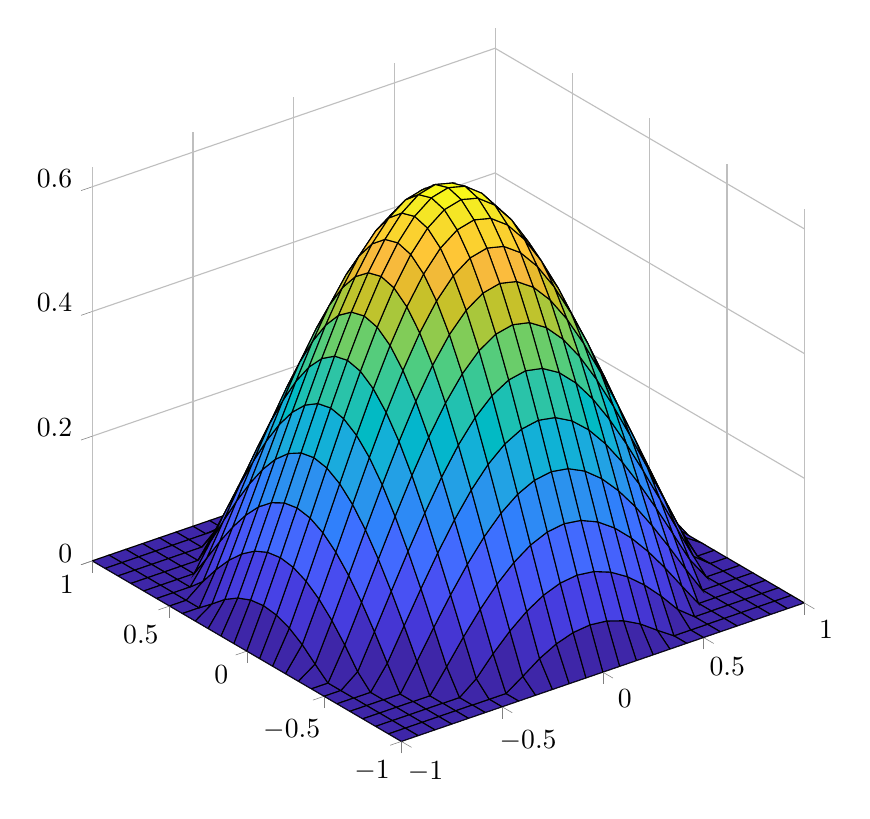
\begin{tikzpicture}

\begin{axis}[%
width=3.56in,
height=3.566in,
at={(0.597in,0.481in)},
scale only axis,
xmin=-1,
xmax=1,
tick align=outside,
ymin=-1,
ymax=1,
zmin=0,
zmax=0.632120558828558,
view={-37.5}{30},
axis background/.style={fill=white},
axis x line*=bottom,
axis y line*=left,
axis z line*=left,
xmajorgrids,
ymajorgrids,
zmajorgrids,
legend style={at={(1.03,1)}, anchor=north west, legend cell align=left, align=left, draw=white!15!black}
]

\addplot3[%
surf,
shader=flat corner, draw=black, z buffer=sort, colormap={mymap}{[1pt] rgb(0pt)=(0.2422,0.1504,0.6603); rgb(1pt)=(0.25039,0.164995,0.707614); rgb(2pt)=(0.257771,0.181781,0.751138); rgb(3pt)=(0.264729,0.197757,0.795214); rgb(4pt)=(0.270648,0.214676,0.836371); rgb(5pt)=(0.275114,0.234238,0.870986); rgb(6pt)=(0.2783,0.255871,0.899071); rgb(7pt)=(0.280333,0.278233,0.9221); rgb(8pt)=(0.281338,0.300595,0.941376); rgb(9pt)=(0.281014,0.322757,0.957886); rgb(10pt)=(0.279467,0.344671,0.971676); rgb(11pt)=(0.275971,0.366681,0.982905); rgb(12pt)=(0.269914,0.3892,0.9906); rgb(13pt)=(0.260243,0.412329,0.995157); rgb(14pt)=(0.244033,0.435833,0.998833); rgb(15pt)=(0.220643,0.460257,0.997286); rgb(16pt)=(0.196333,0.484719,0.989152); rgb(17pt)=(0.183405,0.507371,0.979795); rgb(18pt)=(0.178643,0.528857,0.968157); rgb(19pt)=(0.176438,0.549905,0.952019); rgb(20pt)=(0.168743,0.570262,0.935871); rgb(21pt)=(0.154,0.5902,0.9218); rgb(22pt)=(0.146029,0.609119,0.907857); rgb(23pt)=(0.138024,0.627629,0.89729); rgb(24pt)=(0.124814,0.645929,0.888343); rgb(25pt)=(0.111252,0.6635,0.876314); rgb(26pt)=(0.0952095,0.679829,0.859781); rgb(27pt)=(0.0688714,0.694771,0.839357); rgb(28pt)=(0.0296667,0.708167,0.816333); rgb(29pt)=(0.00357143,0.720267,0.7917); rgb(30pt)=(0.00665714,0.731214,0.766014); rgb(31pt)=(0.0433286,0.741095,0.73941); rgb(32pt)=(0.0963952,0.75,0.712038); rgb(33pt)=(0.140771,0.7584,0.684157); rgb(34pt)=(0.1717,0.766962,0.655443); rgb(35pt)=(0.193767,0.775767,0.6251); rgb(36pt)=(0.216086,0.7843,0.5923); rgb(37pt)=(0.246957,0.791795,0.556743); rgb(38pt)=(0.290614,0.79729,0.518829); rgb(39pt)=(0.340643,0.8008,0.478857); rgb(40pt)=(0.3909,0.802871,0.435448); rgb(41pt)=(0.445629,0.802419,0.390919); rgb(42pt)=(0.5044,0.7993,0.348); rgb(43pt)=(0.561562,0.794233,0.304481); rgb(44pt)=(0.617395,0.787619,0.261238); rgb(45pt)=(0.671986,0.779271,0.2227); rgb(46pt)=(0.7242,0.769843,0.191029); rgb(47pt)=(0.773833,0.759805,0.16461); rgb(48pt)=(0.820314,0.749814,0.153529); rgb(49pt)=(0.863433,0.7406,0.159633); rgb(50pt)=(0.903543,0.733029,0.177414); rgb(51pt)=(0.939257,0.728786,0.209957); rgb(52pt)=(0.972757,0.729771,0.239443); rgb(53pt)=(0.995648,0.743371,0.237148); rgb(54pt)=(0.996986,0.765857,0.219943); rgb(55pt)=(0.995205,0.789252,0.202762); rgb(56pt)=(0.9892,0.813567,0.188533); rgb(57pt)=(0.978629,0.838629,0.176557); rgb(58pt)=(0.967648,0.8639,0.16429); rgb(59pt)=(0.96101,0.889019,0.153676); rgb(60pt)=(0.959671,0.913457,0.142257); rgb(61pt)=(0.962795,0.937338,0.12651); rgb(62pt)=(0.969114,0.960629,0.106362); rgb(63pt)=(0.9769,0.9839,0.0805)}, mesh/rows=25]
table[row sep=crcr, point meta=\thisrow{c}] {%
%
x	y	z	c\\
-1	-1	0	0\\
-0.916666666666667	-1	0	0\\
-0.833333333333333	-1	0	0\\
-0.75	-1	0	0\\
-0.666666666666667	-1	0	0\\
-0.583333333333333	-1	0	0\\
-0.5	-1	0	0\\
-0.416666666666667	-1	0	0\\
-0.333333333333333	-1	0	0\\
-0.25	-1	0	0\\
-0.166666666666667	-1	0	0\\
-0.0833333333333334	-1	0	0\\
0	-1	5.55111512312578e-17	5.55111512312578e-17\\
0.0833333333333333	-1	0	0\\
0.166666666666667	-1	0	0\\
0.25	-1	0	0\\
0.333333333333333	-1	0	0\\
0.416666666666667	-1	0	0\\
0.5	-1	0	0\\
0.583333333333333	-1	0	0\\
0.666666666666667	-1	0	0\\
0.75	-1	0	0\\
0.833333333333333	-1	0	0\\
0.916666666666667	-1	0	0\\
1	-1	0	0\\
-1	-0.916666666666667	0	0\\
-0.916666666666667	-0.916666666666667	0	0\\
-0.833333333333333	-0.916666666666667	0	0\\
-0.75	-0.916666666666667	0	0\\
-0.666666666666667	-0.916666666666667	0	0\\
-0.583333333333333	-0.916666666666667	0	0\\
-0.5	-0.916666666666667	0	0\\
-0.416666666666667	-0.916666666666667	0	0\\
-0.333333333333333	-0.916666666666667	0.0183248148141781	0.0183248148141781\\
-0.25	-0.916666666666667	0.0375624255076384	0.0375624255076384\\
-0.166666666666667	-0.916666666666667	0.0518875286016618	0.0518875286016618\\
-0.0833333333333334	-0.916666666666667	0.0607244049823947	0.0607244049823947\\
0	-0.916666666666667	0.0637111793217526	0.0637111793217526\\
0.0833333333333333	-0.916666666666667	0.0607244049823947	0.0607244049823947\\
0.166666666666667	-0.916666666666667	0.0518875286016618	0.0518875286016618\\
0.25	-0.916666666666667	0.0375624255076384	0.0375624255076384\\
0.333333333333333	-0.916666666666667	0.0183248148141782	0.0183248148141782\\
0.416666666666667	-0.916666666666667	0	0\\
0.5	-0.916666666666667	0	0\\
0.583333333333333	-0.916666666666667	0	0\\
0.666666666666667	-0.916666666666667	0	0\\
0.75	-0.916666666666667	0	0\\
0.833333333333333	-0.916666666666667	0	0\\
0.916666666666667	-0.916666666666667	0	0\\
1	-0.916666666666667	0	0\\
-1	-0.833333333333333	0	0\\
-0.916666666666667	-0.833333333333333	0	0\\
-0.833333333333333	-0.833333333333333	0	0\\
-0.75	-0.833333333333333	0	0\\
-0.666666666666667	-0.833333333333333	0	0\\
-0.583333333333333	-0.833333333333333	0	0\\
-0.5	-0.833333333333333	0.0210161228177806	0.0210161228177806\\
-0.416666666666667	-0.833333333333333	0.0518875286016618	0.0518875286016618\\
-0.333333333333333	-0.833333333333333	0.0789601721887676	0.0789601721887676\\
-0.25	-0.833333333333333	0.101218151977991	0.101218151977991\\
-0.166666666666667	-0.833333333333333	0.11779234407627	0.11779234407627\\
-0.0833333333333334	-0.833333333333333	0.128016639547073	0.128016639547073\\
0	-0.833333333333333	0.131472347427834	0.131472347427834\\
0.0833333333333333	-0.833333333333333	0.128016639547073	0.128016639547073\\
0.166666666666667	-0.833333333333333	0.11779234407627	0.11779234407627\\
0.25	-0.833333333333333	0.101218151977991	0.101218151977991\\
0.333333333333333	-0.833333333333333	0.0789601721887676	0.0789601721887676\\
0.416666666666667	-0.833333333333333	0.0518875286016617	0.0518875286016617\\
0.5	-0.833333333333333	0.0210161228177806	0.0210161228177806\\
0.583333333333333	-0.833333333333333	0	0\\
0.666666666666667	-0.833333333333333	0	0\\
0.75	-0.833333333333333	0	0\\
0.833333333333333	-0.833333333333333	0	0\\
0.916666666666667	-0.833333333333333	0	0\\
1	-0.833333333333333	0	0\\
-1	-0.75	0	0\\
-0.916666666666667	-0.75	0	0\\
-0.833333333333333	-0.75	0	0\\
-0.75	-0.75	0	0\\
-0.666666666666667	-0.75	0	0\\
-0.583333333333333	-0.75	0.0375624255076384	0.0375624255076384\\
-0.5	-0.75	0.0758678689096376	0.0758678689096376\\
-0.416666666666667	-0.75	0.111093529841575	0.111093529841575\\
-0.333333333333333	-0.75	0.141984632443339	0.141984632443339\\
-0.25	-0.75	0.167381987347548	0.167381987347548\\
-0.166666666666667	-0.75	0.186293885145853	0.186293885145853\\
-0.0833333333333334	-0.75	0.19796026561598	0.19796026561598\\
0	-0.75	0.201903383559481	0.201903383559481\\
0.0833333333333333	-0.75	0.19796026561598	0.19796026561598\\
0.166666666666667	-0.75	0.186293885145853	0.186293885145853\\
0.25	-0.75	0.167381987347548	0.167381987347548\\
0.333333333333333	-0.75	0.141984632443339	0.141984632443339\\
0.416666666666667	-0.75	0.111093529841575	0.111093529841575\\
0.5	-0.75	0.0758678689096376	0.0758678689096376\\
0.583333333333333	-0.75	0.0375624255076384	0.0375624255076384\\
0.666666666666667	-0.75	0	0\\
0.75	-0.75	0	0\\
0.833333333333333	-0.75	0	0\\
0.916666666666667	-0.75	0	0\\
1	-0.75	0	0\\
-1	-0.666666666666667	0	0\\
-0.916666666666667	-0.666666666666667	0	0\\
-0.833333333333333	-0.666666666666667	0	0\\
-0.75	-0.666666666666667	0	0\\
-0.666666666666667	-0.666666666666667	0.0432328493357451	0.0432328493357451\\
-0.583333333333333	-0.666666666666667	0.0883669781301998	0.0883669781301998\\
-0.5	-0.666666666666667	0.131472347427834	0.131472347427834\\
-0.416666666666667	-0.666666666666667	0.171112017103218	0.171112017103218\\
-0.333333333333333	-0.666666666666667	0.20587397956599	0.20587397956599\\
-0.25	-0.666666666666667	0.234453791339475	0.234453791339475\\
-0.166666666666667	-0.666666666666667	0.255735475254731	0.255735475254731\\
-0.0833333333333334	-0.666666666666667	0.268863730506967	0.268863730506967\\
0	-0.666666666666667	0.273300947258512	0.273300947258512\\
0.0833333333333333	-0.666666666666667	0.268863730506967	0.268863730506967\\
0.166666666666667	-0.666666666666667	0.255735475254731	0.255735475254731\\
0.25	-0.666666666666667	0.234453791339475	0.234453791339475\\
0.333333333333333	-0.666666666666667	0.20587397956599	0.20587397956599\\
0.416666666666667	-0.666666666666667	0.171112017103218	0.171112017103218\\
0.5	-0.666666666666667	0.131472347427834	0.131472347427834\\
0.583333333333333	-0.666666666666667	0.0883669781301998	0.0883669781301998\\
0.666666666666667	-0.666666666666667	0.0432328493357451	0.0432328493357451\\
0.75	-0.666666666666667	0	0\\
0.833333333333333	-0.666666666666667	0	0\\
0.916666666666667	-0.666666666666667	0	0\\
1	-0.666666666666667	0	0\\
-1	-0.583333333333333	0	0\\
-0.916666666666667	-0.583333333333333	0	0\\
-0.833333333333333	-0.583333333333333	0	0\\
-0.75	-0.583333333333333	0.0375624255076384	0.0375624255076384\\
-0.666666666666667	-0.583333333333333	0.0883669781301998	0.0883669781301998\\
-0.583333333333333	-0.583333333333333	0.138456175476658	0.138456175476658\\
-0.5	-0.583333333333333	0.186293885145853	0.186293885145853\\
-0.416666666666667	-0.583333333333333	0.230285411960539	0.230285411960539\\
-0.333333333333333	-0.583333333333333	0.268863730506967	0.268863730506967\\
-0.25	-0.583333333333333	0.300581188454723	0.300581188454723\\
-0.166666666666667	-0.583333333333333	0.324199290630812	0.324199290630812\\
-0.0833333333333334	-0.583333333333333	0.338768836686274	0.338768836686274\\
0	-0.583333333333333	0.343693195070355	0.343693195070355\\
0.0833333333333333	-0.583333333333333	0.338768836686274	0.338768836686274\\
0.166666666666667	-0.583333333333333	0.324199290630812	0.324199290630812\\
0.25	-0.583333333333333	0.300581188454723	0.300581188454723\\
0.333333333333333	-0.583333333333333	0.268863730506967	0.268863730506967\\
0.416666666666667	-0.583333333333333	0.230285411960539	0.230285411960539\\
0.5	-0.583333333333333	0.186293885145853	0.186293885145853\\
0.583333333333333	-0.583333333333333	0.138456175476658	0.138456175476658\\
0.666666666666667	-0.583333333333333	0.0883669781301998	0.0883669781301998\\
0.75	-0.583333333333333	0.0375624255076384	0.0375624255076384\\
0.833333333333333	-0.583333333333333	0	0\\
0.916666666666667	-0.583333333333333	0	0\\
1	-0.583333333333333	0	0\\
-1	-0.5	0	0\\
-0.916666666666667	-0.5	0	0\\
-0.833333333333333	-0.5	0.0210161228177806	0.0210161228177806\\
-0.75	-0.5	0.0758678689096376	0.0758678689096376\\
-0.666666666666667	-0.5	0.131472347427834	0.131472347427834\\
-0.583333333333333	-0.5	0.186293885145853	0.186293885145853\\
-0.5	-0.5	0.238651218541191	0.238651218541191\\
-0.416666666666667	-0.5	0.286798988405886	0.286798988405886\\
-0.333333333333333	-0.5	0.32902211948667	0.32902211948667\\
-0.25	-0.5	0.3637361877752	0.3637361877752\\
-0.166666666666667	-0.5	0.389585687225524	0.389585687225524\\
-0.0833333333333334	-0.5	0.405531738688263	0.405531738688263\\
0	-0.5	0.410921341899963	0.410921341899963\\
0.0833333333333333	-0.5	0.405531738688263	0.405531738688263\\
0.166666666666667	-0.5	0.389585687225524	0.389585687225524\\
0.25	-0.5	0.3637361877752	0.3637361877752\\
0.333333333333333	-0.5	0.32902211948667	0.32902211948667\\
0.416666666666667	-0.5	0.286798988405886	0.286798988405886\\
0.5	-0.5	0.238651218541191	0.238651218541191\\
0.583333333333333	-0.5	0.186293885145853	0.186293885145853\\
0.666666666666667	-0.5	0.131472347427834	0.131472347427834\\
0.75	-0.5	0.0758678689096376	0.0758678689096376\\
0.833333333333333	-0.5	0.0210161228177807	0.0210161228177807\\
0.916666666666667	-0.5	0	0\\
1	-0.5	0	0\\
-1	-0.416666666666667	0	0\\
-0.916666666666667	-0.416666666666667	0	0\\
-0.833333333333333	-0.416666666666667	0.0518875286016618	0.0518875286016618\\
-0.75	-0.416666666666667	0.111093529841575	0.111093529841575\\
-0.666666666666667	-0.416666666666667	0.171112017103218	0.171112017103218\\
-0.583333333333333	-0.416666666666667	0.230285411960539	0.230285411960539\\
-0.5	-0.416666666666667	0.286798988405886	0.286798988405886\\
-0.416666666666667	-0.416666666666667	0.338768836686274	0.338768836686274\\
-0.333333333333333	-0.416666666666667	0.384343735011945	0.384343735011945\\
-0.25	-0.416666666666667	0.421813484228155	0.421813484228155\\
-0.166666666666667	-0.416666666666667	0.449714975166002	0.449714975166002\\
-0.0833333333333334	-0.416666666666667	0.466926860109347	0.466926860109347\\
0	-0.416666666666667	0.472744302163063	0.472744302163063\\
0.0833333333333333	-0.416666666666667	0.466926860109347	0.466926860109347\\
0.166666666666667	-0.416666666666667	0.449714975166002	0.449714975166002\\
0.25	-0.416666666666667	0.421813484228155	0.421813484228155\\
0.333333333333333	-0.416666666666667	0.384343735011945	0.384343735011945\\
0.416666666666667	-0.416666666666667	0.338768836686274	0.338768836686274\\
0.5	-0.416666666666667	0.286798988405886	0.286798988405886\\
0.583333333333333	-0.416666666666667	0.230285411960539	0.230285411960539\\
0.666666666666667	-0.416666666666667	0.171112017103218	0.171112017103218\\
0.75	-0.416666666666667	0.111093529841575	0.111093529841575\\
0.833333333333333	-0.416666666666667	0.0518875286016619	0.0518875286016619\\
0.916666666666667	-0.416666666666667	0	0\\
1	-0.416666666666667	0	0\\
-1	-0.333333333333333	0	0\\
-0.916666666666667	-0.333333333333333	0.0183248148141781	0.0183248148141781\\
-0.833333333333333	-0.333333333333333	0.0789601721887676	0.0789601721887676\\
-0.75	-0.333333333333333	0.141984632443339	0.141984632443339\\
-0.666666666666667	-0.333333333333333	0.20587397956599	0.20587397956599\\
-0.583333333333333	-0.333333333333333	0.268863730506967	0.268863730506967\\
-0.5	-0.333333333333333	0.32902211948667	0.32902211948667\\
-0.416666666666667	-0.333333333333333	0.384343735011945	0.384343735011945\\
-0.333333333333333	-0.333333333333333	0.432857961745366	0.432857961745366\\
-0.25	-0.333333333333333	0.472744302163063	0.472744302163063\\
-0.166666666666667	-0.333333333333333	0.502445284661948	0.502445284661948\\
-0.0833333333333334	-0.333333333333333	0.520767240811671	0.520767240811671\\
0	-0.333333333333333	0.526959875642927	0.526959875642927\\
0.0833333333333333	-0.333333333333333	0.520767240811671	0.520767240811671\\
0.166666666666667	-0.333333333333333	0.502445284661948	0.502445284661948\\
0.25	-0.333333333333333	0.472744302163063	0.472744302163063\\
0.333333333333333	-0.333333333333333	0.432857961745366	0.432857961745366\\
0.416666666666667	-0.333333333333333	0.384343735011945	0.384343735011945\\
0.5	-0.333333333333333	0.32902211948667	0.32902211948667\\
0.583333333333333	-0.333333333333333	0.268863730506967	0.268863730506967\\
0.666666666666667	-0.333333333333333	0.20587397956599	0.20587397956599\\
0.75	-0.333333333333333	0.141984632443339	0.141984632443339\\
0.833333333333333	-0.333333333333333	0.0789601721887677	0.0789601721887677\\
0.916666666666667	-0.333333333333333	0.018324814814178	0.018324814814178\\
1	-0.333333333333333	0	0\\
-1	-0.25	0	0\\
-0.916666666666667	-0.25	0.0375624255076384	0.0375624255076384\\
-0.833333333333333	-0.25	0.101218151977991	0.101218151977991\\
-0.75	-0.25	0.167381987347548	0.167381987347548\\
-0.666666666666667	-0.25	0.234453791339475	0.234453791339475\\
-0.583333333333333	-0.25	0.300581188454723	0.300581188454723\\
-0.5	-0.25	0.3637361877752	0.3637361877752\\
-0.416666666666667	-0.25	0.421813484228155	0.421813484228155\\
-0.333333333333333	-0.25	0.472744302163063	0.472744302163063\\
-0.25	-0.25	0.514617461413153	0.514617461413153\\
-0.166666666666667	-0.25	0.545797909582526	0.545797909582526\\
-0.0833333333333334	-0.25	0.565032519215705	0.565032519215705\\
0	-0.25	0.571533621642033	0.571533621642033\\
0.0833333333333333	-0.25	0.565032519215705	0.565032519215705\\
0.166666666666667	-0.25	0.545797909582526	0.545797909582526\\
0.25	-0.25	0.514617461413153	0.514617461413153\\
0.333333333333333	-0.25	0.472744302163063	0.472744302163063\\
0.416666666666667	-0.25	0.421813484228155	0.421813484228155\\
0.5	-0.25	0.3637361877752	0.3637361877752\\
0.583333333333333	-0.25	0.300581188454723	0.300581188454723\\
0.666666666666667	-0.25	0.234453791339475	0.234453791339475\\
0.75	-0.25	0.167381987347548	0.167381987347548\\
0.833333333333333	-0.25	0.101218151977991	0.101218151977991\\
0.916666666666667	-0.25	0.0375624255076383	0.0375624255076383\\
1	-0.25	0	0\\
-1	-0.166666666666667	0	0\\
-0.916666666666667	-0.166666666666667	0.0518875286016618	0.0518875286016618\\
-0.833333333333333	-0.166666666666667	0.11779234407627	0.11779234407627\\
-0.75	-0.166666666666667	0.186293885145853	0.186293885145853\\
-0.666666666666667	-0.166666666666667	0.255735475254731	0.255735475254731\\
-0.583333333333333	-0.166666666666667	0.324199290630812	0.324199290630812\\
-0.5	-0.166666666666667	0.389585687225524	0.389585687225524\\
-0.416666666666667	-0.166666666666667	0.449714975166002	0.449714975166002\\
-0.333333333333333	-0.166666666666667	0.502445284661948	0.502445284661948\\
-0.25	-0.166666666666667	0.545797909582526	0.545797909582526\\
-0.166666666666667	-0.166666666666667	0.578080027735323	0.578080027735323\\
-0.0833333333333334	-0.166666666666667	0.597994236069607	0.597994236069607\\
0	-0.166666666666667	0.604725035944906	0.604725035944906\\
0.0833333333333333	-0.166666666666667	0.597994236069607	0.597994236069607\\
0.166666666666667	-0.166666666666667	0.578080027735323	0.578080027735323\\
0.25	-0.166666666666667	0.545797909582526	0.545797909582526\\
0.333333333333333	-0.166666666666667	0.502445284661948	0.502445284661948\\
0.416666666666667	-0.166666666666667	0.449714975166002	0.449714975166002\\
0.5	-0.166666666666667	0.389585687225524	0.389585687225524\\
0.583333333333333	-0.166666666666667	0.324199290630812	0.324199290630812\\
0.666666666666667	-0.166666666666667	0.255735475254731	0.255735475254731\\
0.75	-0.166666666666667	0.186293885145853	0.186293885145853\\
0.833333333333333	-0.166666666666667	0.11779234407627	0.11779234407627\\
0.916666666666667	-0.166666666666667	0.0518875286016617	0.0518875286016617\\
1	-0.166666666666667	0	0\\
-1	-0.0833333333333334	0	0\\
-0.916666666666667	-0.0833333333333334	0.0607244049823947	0.0607244049823947\\
-0.833333333333333	-0.0833333333333334	0.128016639547073	0.128016639547073\\
-0.75	-0.0833333333333334	0.19796026561598	0.19796026561598\\
-0.666666666666667	-0.0833333333333334	0.268863730506967	0.268863730506967\\
-0.583333333333333	-0.0833333333333334	0.338768836686274	0.338768836686274\\
-0.5	-0.0833333333333334	0.405531738688263	0.405531738688263\\
-0.416666666666667	-0.0833333333333334	0.466926860109347	0.466926860109347\\
-0.333333333333333	-0.0833333333333334	0.520767240811671	0.520767240811671\\
-0.25	-0.0833333333333334	0.565032519215705	0.565032519215705\\
-0.166666666666667	-0.0833333333333334	0.597994236069607	0.597994236069607\\
-0.0833333333333334	-0.0833333333333334	0.618327675572474	0.618327675572474\\
0	-0.0833333333333334	0.625200171318874	0.625200171318874\\
0.0833333333333333	-0.0833333333333334	0.618327675572474	0.618327675572474\\
0.166666666666667	-0.0833333333333334	0.597994236069607	0.597994236069607\\
0.25	-0.0833333333333334	0.565032519215705	0.565032519215705\\
0.333333333333333	-0.0833333333333334	0.520767240811671	0.520767240811671\\
0.416666666666667	-0.0833333333333334	0.466926860109347	0.466926860109347\\
0.5	-0.0833333333333334	0.405531738688263	0.405531738688263\\
0.583333333333333	-0.0833333333333334	0.338768836686274	0.338768836686274\\
0.666666666666667	-0.0833333333333334	0.268863730506967	0.268863730506967\\
0.75	-0.0833333333333334	0.19796026561598	0.19796026561598\\
0.833333333333333	-0.0833333333333334	0.128016639547073	0.128016639547073\\
0.916666666666667	-0.0833333333333334	0.0607244049823946	0.0607244049823946\\
1	-0.0833333333333334	0	0\\
-1	0	5.55111512312578e-17	5.55111512312578e-17\\
-0.916666666666667	0	0.0637111793217526	0.0637111793217526\\
-0.833333333333333	0	0.131472347427834	0.131472347427834\\
-0.75	0	0.201903383559481	0.201903383559481\\
-0.666666666666667	0	0.273300947258512	0.273300947258512\\
-0.583333333333333	0	0.343693195070355	0.343693195070355\\
-0.5	0	0.410921341899963	0.410921341899963\\
-0.416666666666667	0	0.472744302163063	0.472744302163063\\
-0.333333333333333	0	0.526959875642927	0.526959875642927\\
-0.25	0	0.571533621642033	0.571533621642033\\
-0.166666666666667	0	0.604725035944906	0.604725035944906\\
-0.0833333333333334	0	0.625200171318874	0.625200171318874\\
0	0	0.632120558828558	0.632120558828558\\
0.0833333333333333	0	0.625200171318874	0.625200171318874\\
0.166666666666667	0	0.604725035944906	0.604725035944906\\
0.25	0	0.571533621642033	0.571533621642033\\
0.333333333333333	0	0.526959875642927	0.526959875642927\\
0.416666666666667	0	0.472744302163063	0.472744302163063\\
0.5	0	0.410921341899963	0.410921341899963\\
0.583333333333333	0	0.343693195070355	0.343693195070355\\
0.666666666666667	0	0.273300947258512	0.273300947258512\\
0.75	0	0.201903383559481	0.201903383559481\\
0.833333333333333	0	0.131472347427834	0.131472347427834\\
0.916666666666667	0	0.0637111793217525	0.0637111793217525\\
1	0	5.55111512312578e-17	5.55111512312578e-17\\
-1	0.0833333333333333	0	0\\
-0.916666666666667	0.0833333333333333	0.0607244049823947	0.0607244049823947\\
-0.833333333333333	0.0833333333333333	0.128016639547073	0.128016639547073\\
-0.75	0.0833333333333333	0.19796026561598	0.19796026561598\\
-0.666666666666667	0.0833333333333333	0.268863730506967	0.268863730506967\\
-0.583333333333333	0.0833333333333333	0.338768836686274	0.338768836686274\\
-0.5	0.0833333333333333	0.405531738688263	0.405531738688263\\
-0.416666666666667	0.0833333333333333	0.466926860109347	0.466926860109347\\
-0.333333333333333	0.0833333333333333	0.520767240811671	0.520767240811671\\
-0.25	0.0833333333333333	0.565032519215705	0.565032519215705\\
-0.166666666666667	0.0833333333333333	0.597994236069607	0.597994236069607\\
-0.0833333333333334	0.0833333333333333	0.618327675572474	0.618327675572474\\
0	0.0833333333333333	0.625200171318874	0.625200171318874\\
0.0833333333333333	0.0833333333333333	0.618327675572474	0.618327675572474\\
0.166666666666667	0.0833333333333333	0.597994236069607	0.597994236069607\\
0.25	0.0833333333333333	0.565032519215705	0.565032519215705\\
0.333333333333333	0.0833333333333333	0.520767240811671	0.520767240811671\\
0.416666666666667	0.0833333333333333	0.466926860109347	0.466926860109347\\
0.5	0.0833333333333333	0.405531738688263	0.405531738688263\\
0.583333333333333	0.0833333333333333	0.338768836686274	0.338768836686274\\
0.666666666666667	0.0833333333333333	0.268863730506967	0.268863730506967\\
0.75	0.0833333333333333	0.19796026561598	0.19796026561598\\
0.833333333333333	0.0833333333333333	0.128016639547073	0.128016639547073\\
0.916666666666667	0.0833333333333333	0.0607244049823946	0.0607244049823946\\
1	0.0833333333333333	0	0\\
-1	0.166666666666667	0	0\\
-0.916666666666667	0.166666666666667	0.0518875286016618	0.0518875286016618\\
-0.833333333333333	0.166666666666667	0.11779234407627	0.11779234407627\\
-0.75	0.166666666666667	0.186293885145853	0.186293885145853\\
-0.666666666666667	0.166666666666667	0.255735475254731	0.255735475254731\\
-0.583333333333333	0.166666666666667	0.324199290630812	0.324199290630812\\
-0.5	0.166666666666667	0.389585687225524	0.389585687225524\\
-0.416666666666667	0.166666666666667	0.449714975166002	0.449714975166002\\
-0.333333333333333	0.166666666666667	0.502445284661948	0.502445284661948\\
-0.25	0.166666666666667	0.545797909582526	0.545797909582526\\
-0.166666666666667	0.166666666666667	0.578080027735323	0.578080027735323\\
-0.0833333333333334	0.166666666666667	0.597994236069607	0.597994236069607\\
0	0.166666666666667	0.604725035944906	0.604725035944906\\
0.0833333333333333	0.166666666666667	0.597994236069607	0.597994236069607\\
0.166666666666667	0.166666666666667	0.578080027735323	0.578080027735323\\
0.25	0.166666666666667	0.545797909582526	0.545797909582526\\
0.333333333333333	0.166666666666667	0.502445284661948	0.502445284661948\\
0.416666666666667	0.166666666666667	0.449714975166002	0.449714975166002\\
0.5	0.166666666666667	0.389585687225524	0.389585687225524\\
0.583333333333333	0.166666666666667	0.324199290630812	0.324199290630812\\
0.666666666666667	0.166666666666667	0.255735475254731	0.255735475254731\\
0.75	0.166666666666667	0.186293885145853	0.186293885145853\\
0.833333333333333	0.166666666666667	0.11779234407627	0.11779234407627\\
0.916666666666667	0.166666666666667	0.0518875286016617	0.0518875286016617\\
1	0.166666666666667	0	0\\
-1	0.25	0	0\\
-0.916666666666667	0.25	0.0375624255076384	0.0375624255076384\\
-0.833333333333333	0.25	0.101218151977991	0.101218151977991\\
-0.75	0.25	0.167381987347548	0.167381987347548\\
-0.666666666666667	0.25	0.234453791339475	0.234453791339475\\
-0.583333333333333	0.25	0.300581188454723	0.300581188454723\\
-0.5	0.25	0.3637361877752	0.3637361877752\\
-0.416666666666667	0.25	0.421813484228155	0.421813484228155\\
-0.333333333333333	0.25	0.472744302163063	0.472744302163063\\
-0.25	0.25	0.514617461413153	0.514617461413153\\
-0.166666666666667	0.25	0.545797909582526	0.545797909582526\\
-0.0833333333333334	0.25	0.565032519215705	0.565032519215705\\
0	0.25	0.571533621642033	0.571533621642033\\
0.0833333333333333	0.25	0.565032519215705	0.565032519215705\\
0.166666666666667	0.25	0.545797909582526	0.545797909582526\\
0.25	0.25	0.514617461413153	0.514617461413153\\
0.333333333333333	0.25	0.472744302163063	0.472744302163063\\
0.416666666666667	0.25	0.421813484228155	0.421813484228155\\
0.5	0.25	0.3637361877752	0.3637361877752\\
0.583333333333333	0.25	0.300581188454723	0.300581188454723\\
0.666666666666667	0.25	0.234453791339475	0.234453791339475\\
0.75	0.25	0.167381987347548	0.167381987347548\\
0.833333333333333	0.25	0.101218151977991	0.101218151977991\\
0.916666666666667	0.25	0.0375624255076383	0.0375624255076383\\
1	0.25	0	0\\
-1	0.333333333333333	0	0\\
-0.916666666666667	0.333333333333333	0.0183248148141782	0.0183248148141782\\
-0.833333333333333	0.333333333333333	0.0789601721887676	0.0789601721887676\\
-0.75	0.333333333333333	0.141984632443339	0.141984632443339\\
-0.666666666666667	0.333333333333333	0.20587397956599	0.20587397956599\\
-0.583333333333333	0.333333333333333	0.268863730506967	0.268863730506967\\
-0.5	0.333333333333333	0.32902211948667	0.32902211948667\\
-0.416666666666667	0.333333333333333	0.384343735011945	0.384343735011945\\
-0.333333333333333	0.333333333333333	0.432857961745366	0.432857961745366\\
-0.25	0.333333333333333	0.472744302163063	0.472744302163063\\
-0.166666666666667	0.333333333333333	0.502445284661948	0.502445284661948\\
-0.0833333333333334	0.333333333333333	0.520767240811671	0.520767240811671\\
0	0.333333333333333	0.526959875642927	0.526959875642927\\
0.0833333333333333	0.333333333333333	0.520767240811671	0.520767240811671\\
0.166666666666667	0.333333333333333	0.502445284661948	0.502445284661948\\
0.25	0.333333333333333	0.472744302163063	0.472744302163063\\
0.333333333333333	0.333333333333333	0.432857961745366	0.432857961745366\\
0.416666666666667	0.333333333333333	0.384343735011945	0.384343735011945\\
0.5	0.333333333333333	0.32902211948667	0.32902211948667\\
0.583333333333333	0.333333333333333	0.268863730506967	0.268863730506967\\
0.666666666666667	0.333333333333333	0.20587397956599	0.20587397956599\\
0.75	0.333333333333333	0.141984632443339	0.141984632443339\\
0.833333333333333	0.333333333333333	0.0789601721887677	0.0789601721887677\\
0.916666666666667	0.333333333333333	0.0183248148141781	0.0183248148141781\\
1	0.333333333333333	0	0\\
-1	0.416666666666667	0	0\\
-0.916666666666667	0.416666666666667	0	0\\
-0.833333333333333	0.416666666666667	0.0518875286016617	0.0518875286016617\\
-0.75	0.416666666666667	0.111093529841575	0.111093529841575\\
-0.666666666666667	0.416666666666667	0.171112017103218	0.171112017103218\\
-0.583333333333333	0.416666666666667	0.230285411960539	0.230285411960539\\
-0.5	0.416666666666667	0.286798988405886	0.286798988405886\\
-0.416666666666667	0.416666666666667	0.338768836686274	0.338768836686274\\
-0.333333333333333	0.416666666666667	0.384343735011945	0.384343735011945\\
-0.25	0.416666666666667	0.421813484228155	0.421813484228155\\
-0.166666666666667	0.416666666666667	0.449714975166002	0.449714975166002\\
-0.0833333333333334	0.416666666666667	0.466926860109347	0.466926860109347\\
0	0.416666666666667	0.472744302163063	0.472744302163063\\
0.0833333333333333	0.416666666666667	0.466926860109347	0.466926860109347\\
0.166666666666667	0.416666666666667	0.449714975166002	0.449714975166002\\
0.25	0.416666666666667	0.421813484228155	0.421813484228155\\
0.333333333333333	0.416666666666667	0.384343735011945	0.384343735011945\\
0.416666666666667	0.416666666666667	0.338768836686274	0.338768836686274\\
0.5	0.416666666666667	0.286798988405886	0.286798988405886\\
0.583333333333333	0.416666666666667	0.230285411960539	0.230285411960539\\
0.666666666666667	0.416666666666667	0.171112017103218	0.171112017103218\\
0.75	0.416666666666667	0.111093529841575	0.111093529841575\\
0.833333333333333	0.416666666666667	0.0518875286016618	0.0518875286016618\\
0.916666666666667	0.416666666666667	0	0\\
1	0.416666666666667	0	0\\
-1	0.5	0	0\\
-0.916666666666667	0.5	0	0\\
-0.833333333333333	0.5	0.0210161228177806	0.0210161228177806\\
-0.75	0.5	0.0758678689096376	0.0758678689096376\\
-0.666666666666667	0.5	0.131472347427834	0.131472347427834\\
-0.583333333333333	0.5	0.186293885145853	0.186293885145853\\
-0.5	0.5	0.238651218541191	0.238651218541191\\
-0.416666666666667	0.5	0.286798988405886	0.286798988405886\\
-0.333333333333333	0.5	0.32902211948667	0.32902211948667\\
-0.25	0.5	0.3637361877752	0.3637361877752\\
-0.166666666666667	0.5	0.389585687225524	0.389585687225524\\
-0.0833333333333334	0.5	0.405531738688263	0.405531738688263\\
0	0.5	0.410921341899963	0.410921341899963\\
0.0833333333333333	0.5	0.405531738688263	0.405531738688263\\
0.166666666666667	0.5	0.389585687225524	0.389585687225524\\
0.25	0.5	0.3637361877752	0.3637361877752\\
0.333333333333333	0.5	0.32902211948667	0.32902211948667\\
0.416666666666667	0.5	0.286798988405886	0.286798988405886\\
0.5	0.5	0.238651218541191	0.238651218541191\\
0.583333333333333	0.5	0.186293885145853	0.186293885145853\\
0.666666666666667	0.5	0.131472347427834	0.131472347427834\\
0.75	0.5	0.0758678689096376	0.0758678689096376\\
0.833333333333333	0.5	0.0210161228177807	0.0210161228177807\\
0.916666666666667	0.5	0	0\\
1	0.5	0	0\\
-1	0.583333333333333	0	0\\
-0.916666666666667	0.583333333333333	0	0\\
-0.833333333333333	0.583333333333333	0	0\\
-0.75	0.583333333333333	0.0375624255076384	0.0375624255076384\\
-0.666666666666667	0.583333333333333	0.0883669781301998	0.0883669781301998\\
-0.583333333333333	0.583333333333333	0.138456175476658	0.138456175476658\\
-0.5	0.583333333333333	0.186293885145853	0.186293885145853\\
-0.416666666666667	0.583333333333333	0.230285411960539	0.230285411960539\\
-0.333333333333333	0.583333333333333	0.268863730506967	0.268863730506967\\
-0.25	0.583333333333333	0.300581188454723	0.300581188454723\\
-0.166666666666667	0.583333333333333	0.324199290630812	0.324199290630812\\
-0.0833333333333334	0.583333333333333	0.338768836686274	0.338768836686274\\
0	0.583333333333333	0.343693195070355	0.343693195070355\\
0.0833333333333333	0.583333333333333	0.338768836686274	0.338768836686274\\
0.166666666666667	0.583333333333333	0.324199290630812	0.324199290630812\\
0.25	0.583333333333333	0.300581188454723	0.300581188454723\\
0.333333333333333	0.583333333333333	0.268863730506967	0.268863730506967\\
0.416666666666667	0.583333333333333	0.230285411960539	0.230285411960539\\
0.5	0.583333333333333	0.186293885145853	0.186293885145853\\
0.583333333333333	0.583333333333333	0.138456175476658	0.138456175476658\\
0.666666666666667	0.583333333333333	0.0883669781301998	0.0883669781301998\\
0.75	0.583333333333333	0.0375624255076384	0.0375624255076384\\
0.833333333333333	0.583333333333333	0	0\\
0.916666666666667	0.583333333333333	0	0\\
1	0.583333333333333	0	0\\
-1	0.666666666666667	0	0\\
-0.916666666666667	0.666666666666667	0	0\\
-0.833333333333333	0.666666666666667	0	0\\
-0.75	0.666666666666667	0	0\\
-0.666666666666667	0.666666666666667	0.0432328493357451	0.0432328493357451\\
-0.583333333333333	0.666666666666667	0.0883669781301998	0.0883669781301998\\
-0.5	0.666666666666667	0.131472347427834	0.131472347427834\\
-0.416666666666667	0.666666666666667	0.171112017103218	0.171112017103218\\
-0.333333333333333	0.666666666666667	0.20587397956599	0.20587397956599\\
-0.25	0.666666666666667	0.234453791339475	0.234453791339475\\
-0.166666666666667	0.666666666666667	0.255735475254731	0.255735475254731\\
-0.0833333333333334	0.666666666666667	0.268863730506967	0.268863730506967\\
0	0.666666666666667	0.273300947258512	0.273300947258512\\
0.0833333333333333	0.666666666666667	0.268863730506967	0.268863730506967\\
0.166666666666667	0.666666666666667	0.255735475254731	0.255735475254731\\
0.25	0.666666666666667	0.234453791339475	0.234453791339475\\
0.333333333333333	0.666666666666667	0.20587397956599	0.20587397956599\\
0.416666666666667	0.666666666666667	0.171112017103218	0.171112017103218\\
0.5	0.666666666666667	0.131472347427834	0.131472347427834\\
0.583333333333333	0.666666666666667	0.0883669781301998	0.0883669781301998\\
0.666666666666667	0.666666666666667	0.0432328493357451	0.0432328493357451\\
0.75	0.666666666666667	0	0\\
0.833333333333333	0.666666666666667	0	0\\
0.916666666666667	0.666666666666667	0	0\\
1	0.666666666666667	0	0\\
-1	0.75	0	0\\
-0.916666666666667	0.75	0	0\\
-0.833333333333333	0.75	0	0\\
-0.75	0.75	0	0\\
-0.666666666666667	0.75	0	0\\
-0.583333333333333	0.75	0.0375624255076384	0.0375624255076384\\
-0.5	0.75	0.0758678689096376	0.0758678689096376\\
-0.416666666666667	0.75	0.111093529841575	0.111093529841575\\
-0.333333333333333	0.75	0.141984632443339	0.141984632443339\\
-0.25	0.75	0.167381987347548	0.167381987347548\\
-0.166666666666667	0.75	0.186293885145853	0.186293885145853\\
-0.0833333333333334	0.75	0.19796026561598	0.19796026561598\\
0	0.75	0.201903383559481	0.201903383559481\\
0.0833333333333333	0.75	0.19796026561598	0.19796026561598\\
0.166666666666667	0.75	0.186293885145853	0.186293885145853\\
0.25	0.75	0.167381987347548	0.167381987347548\\
0.333333333333333	0.75	0.141984632443339	0.141984632443339\\
0.416666666666667	0.75	0.111093529841575	0.111093529841575\\
0.5	0.75	0.0758678689096376	0.0758678689096376\\
0.583333333333333	0.75	0.0375624255076384	0.0375624255076384\\
0.666666666666667	0.75	0	0\\
0.75	0.75	0	0\\
0.833333333333333	0.75	0	0\\
0.916666666666667	0.75	0	0\\
1	0.75	0	0\\
-1	0.833333333333333	0	0\\
-0.916666666666667	0.833333333333333	0	0\\
-0.833333333333333	0.833333333333333	0	0\\
-0.75	0.833333333333333	0	0\\
-0.666666666666667	0.833333333333333	0	0\\
-0.583333333333333	0.833333333333333	0	0\\
-0.5	0.833333333333333	0.0210161228177807	0.0210161228177807\\
-0.416666666666667	0.833333333333333	0.0518875286016619	0.0518875286016619\\
-0.333333333333333	0.833333333333333	0.0789601721887677	0.0789601721887677\\
-0.25	0.833333333333333	0.101218151977991	0.101218151977991\\
-0.166666666666667	0.833333333333333	0.11779234407627	0.11779234407627\\
-0.0833333333333334	0.833333333333333	0.128016639547073	0.128016639547073\\
0	0.833333333333333	0.131472347427834	0.131472347427834\\
0.0833333333333333	0.833333333333333	0.128016639547073	0.128016639547073\\
0.166666666666667	0.833333333333333	0.11779234407627	0.11779234407627\\
0.25	0.833333333333333	0.101218151977991	0.101218151977991\\
0.333333333333333	0.833333333333333	0.0789601721887677	0.0789601721887677\\
0.416666666666667	0.833333333333333	0.0518875286016618	0.0518875286016618\\
0.5	0.833333333333333	0.0210161228177807	0.0210161228177807\\
0.583333333333333	0.833333333333333	0	0\\
0.666666666666667	0.833333333333333	0	0\\
0.75	0.833333333333333	0	0\\
0.833333333333333	0.833333333333333	0	0\\
0.916666666666667	0.833333333333333	0	0\\
1	0.833333333333333	0	0\\
-1	0.916666666666667	0	0\\
-0.916666666666667	0.916666666666667	0	0\\
-0.833333333333333	0.916666666666667	0	0\\
-0.75	0.916666666666667	0	0\\
-0.666666666666667	0.916666666666667	0	0\\
-0.583333333333333	0.916666666666667	0	0\\
-0.5	0.916666666666667	0	0\\
-0.416666666666667	0.916666666666667	0	0\\
-0.333333333333333	0.916666666666667	0.018324814814178	0.018324814814178\\
-0.25	0.916666666666667	0.0375624255076383	0.0375624255076383\\
-0.166666666666667	0.916666666666667	0.0518875286016617	0.0518875286016617\\
-0.0833333333333334	0.916666666666667	0.0607244049823946	0.0607244049823946\\
0	0.916666666666667	0.0637111793217525	0.0637111793217525\\
0.0833333333333333	0.916666666666667	0.0607244049823946	0.0607244049823946\\
0.166666666666667	0.916666666666667	0.0518875286016617	0.0518875286016617\\
0.25	0.916666666666667	0.0375624255076383	0.0375624255076383\\
0.333333333333333	0.916666666666667	0.0183248148141781	0.0183248148141781\\
0.416666666666667	0.916666666666667	0	0\\
0.5	0.916666666666667	0	0\\
0.583333333333333	0.916666666666667	0	0\\
0.666666666666667	0.916666666666667	0	0\\
0.75	0.916666666666667	0	0\\
0.833333333333333	0.916666666666667	0	0\\
0.916666666666667	0.916666666666667	0	0\\
1	0.916666666666667	0	0\\
-1	1	0	0\\
-0.916666666666667	1	0	0\\
-0.833333333333333	1	0	0\\
-0.75	1	0	0\\
-0.666666666666667	1	0	0\\
-0.583333333333333	1	0	0\\
-0.5	1	0	0\\
-0.416666666666667	1	0	0\\
-0.333333333333333	1	0	0\\
-0.25	1	0	0\\
-0.166666666666667	1	0	0\\
-0.0833333333333334	1	0	0\\
0	1	5.55111512312578e-17	5.55111512312578e-17\\
0.0833333333333333	1	0	0\\
0.166666666666667	1	0	0\\
0.25	1	0	0\\
0.333333333333333	1	0	0\\
0.416666666666667	1	0	0\\
0.5	1	0	0\\
0.583333333333333	1	0	0\\
0.666666666666667	1	0	0\\
0.75	1	0	0\\
0.833333333333333	1	0	0\\
0.916666666666667	1	0	0\\
1	1	0	0\\
};
%\addlegendentry{data1}

\end{axis}
\end{tikzpicture}%
}
\caption{Lösung der zweiten \acs{PDE}}
\label{fig:pde2sol}
\end{figure}
\end{enumerate}


Die Poisson-Gleichung werden wir mithilfe der Kernkollokation numerisch lösen. Dafür wählen wir den Gauß Kern aus Beispiel \ref{ex:Kern}. Aufgrund der fehlenden Praxisrelevanz werden wir die erste in Kapitel \ref{cha:Implementierung} vorgestellte Methode zur Fehlerberechnung in jeder Iteration nicht betrachten, sondern nur die im Residuum.

\section{Fehler}
\subsection{Absoluter Fehler}

Als Maß des Fehlers unserer numerischen Lösung wollen wir den maximalen absoluten Fehler zur analytischen Lösung berechnen, also
\begin{align*}
\text{error} = \max_{x \in \Omega} |u(x) - s_u (x)|,
\end{align*}
wobei $s_u$ die numerische Lösung bezeichnet. Um den Fehler näherungsweise zu bestimmen, legen wir ein eng gewähltes Gitter an Testpunkten über $\Omega$ und bestimmen ihn an diesen Punkten.

Wir werden die drei in Kapitel \ref{cha:Implementierung} vorgestellten Methoden zur Kollokationspunktwahl testen und miteinander vergleichen. 
\subsubsection{Kollokationspunkte als Gitter}
Wir werden die Kollokationspunkte, so wie die Testpunkte, zunächst, wie in Abbildung \ref{fig:Kollok} gezeigt, in einem Gitter anordnen.
\begin{figure}[ht]
\centering
\resizebox {.8\columnwidth} {!} {
% This file was created by matlab2tikz.
%
%The latest updates can be retrieved from
%  http://www.mathworks.com/matlabcentral/fileexchange/22022-matlab2tikz-matlab2tikz
%where you can also make suggestions and rate matlab2tikz.
%
\definecolor{mycolor1}{rgb}{0.00000,0.44700,0.74100}%
%
\begin{tikzpicture}

\begin{axis}[%
width=4.in,
height=4.in,
at={(0.983in,0.681in)},
scale only axis,
xmin=-1,
xmax=1,
ymin=-1,
ymax=1,
axis background/.style={fill=white},
axis x line*=bottom,
axis y line*=left,
legend style={legend cell align=left, align=left, draw=white!15!black}
]
\addplot [color=red, draw=none, mark=+, mark options={solid, red}]
  table[row sep=crcr]{%
-0.777777777777778	-0.777777777777778\\
-0.555555555555556	-0.777777777777778\\
-0.333333333333333	-0.777777777777778\\
-0.111111111111111	-0.777777777777778\\
0.111111111111111	-0.777777777777778\\
0.333333333333333	-0.777777777777778\\
0.555555555555556	-0.777777777777778\\
0.777777777777778	-0.777777777777778\\
-0.777777777777778	-0.555555555555556\\
-0.555555555555556	-0.555555555555556\\
-0.333333333333333	-0.555555555555556\\
-0.111111111111111	-0.555555555555556\\
0.111111111111111	-0.555555555555556\\
0.333333333333333	-0.555555555555556\\
0.555555555555556	-0.555555555555556\\
0.777777777777778	-0.555555555555556\\
-0.777777777777778	-0.333333333333333\\
-0.555555555555556	-0.333333333333333\\
-0.333333333333333	-0.333333333333333\\
-0.111111111111111	-0.333333333333333\\
0.111111111111111	-0.333333333333333\\
0.333333333333333	-0.333333333333333\\
0.555555555555556	-0.333333333333333\\
0.777777777777778	-0.333333333333333\\
-0.777777777777778	-0.111111111111111\\
-0.555555555555556	-0.111111111111111\\
-0.333333333333333	-0.111111111111111\\
-0.111111111111111	-0.111111111111111\\
0.111111111111111	-0.111111111111111\\
0.333333333333333	-0.111111111111111\\
0.555555555555556	-0.111111111111111\\
0.777777777777778	-0.111111111111111\\
-0.777777777777778	0.111111111111111\\
-0.555555555555556	0.111111111111111\\
-0.333333333333333	0.111111111111111\\
-0.111111111111111	0.111111111111111\\
0.111111111111111	0.111111111111111\\
0.333333333333333	0.111111111111111\\
0.555555555555556	0.111111111111111\\
0.777777777777778	0.111111111111111\\
-0.777777777777778	0.333333333333333\\
-0.555555555555556	0.333333333333333\\
-0.333333333333333	0.333333333333333\\
-0.111111111111111	0.333333333333333\\
0.111111111111111	0.333333333333333\\
0.333333333333333	0.333333333333333\\
0.555555555555556	0.333333333333333\\
0.777777777777778	0.333333333333333\\
-0.777777777777778	0.555555555555556\\
-0.555555555555556	0.555555555555556\\
-0.333333333333333	0.555555555555556\\
-0.111111111111111	0.555555555555556\\
0.111111111111111	0.555555555555556\\
0.333333333333333	0.555555555555556\\
0.555555555555556	0.555555555555556\\
0.777777777777778	0.555555555555556\\
-0.777777777777778	0.777777777777778\\
-0.555555555555556	0.777777777777778\\
-0.333333333333333	0.777777777777778\\
-0.111111111111111	0.777777777777778\\
0.111111111111111	0.777777777777778\\
0.333333333333333	0.777777777777778\\
0.555555555555556	0.777777777777778\\
0.777777777777778	0.777777777777778\\
};
\addlegendentry{Kollokationspunkte}

\addplot [color=blue, draw=none, mark=asterisk, mark options={solid, blue}]
  table[row sep=crcr]{%
-0.5	-0.5\\
0	-0.5\\
0.5	-0.5\\
-0.5	0\\
0	0\\
0.5	0\\
-0.5	0.5\\
0	0.5\\
0.5	0.5\\
};
\addlegendentry{Testpunkte}

\addplot [color=mycolor1, forget plot]
  table[row sep=crcr]{%
-1	-1\\
-1	1\\
1	1\\
1	-1\\
-1	-1\\
};
\end{axis}
\end{tikzpicture}%
}
\caption{Kollokationspunkte}
\label{fig:Kollok}
\end{figure}

Damit können wir uns anschauen, wie sich der Fehler bei Verfeinerung des Gitters verhält. Dieser ist in Abbildung \ref{fig:error} für die vier verschiedenen Verfahren dargestellt. 
\begin{figure}[ht]
\centering
\resizebox {\columnwidth} {!} {
% This file was created by matlab2tikz.
%
%The latest updates can be retrieved from
%  http://www.mathworks.com/matlabcentral/fileexchange/22022-matlab2tikz-matlab2tikz
%where you can also make suggestions and rate matlab2tikz.
%
\definecolor{mycolor1}{rgb}{0.00000,0.44700,0.74100}%
\definecolor{mycolor2}{rgb}{0.85000,0.32500,0.09800}%
\definecolor{mycolor3}{rgb}{0.92900,0.69400,0.12500}%
\definecolor{mycolor4}{rgb}{0.49400,0.18400,0.55600}%
%
\begin{tikzpicture}

\begin{axis}[%
width=4.521in,
height=3.566in,
at={(0.758in,0.481in)},
scale only axis,
xmin=0,
xmax=3000,
xlabel style={font=\color{white!15!black}},
xlabel={Anzahl der Kollokationspunkte},
ymode=log,
ymin=1e-08,
ymax=1,
yminorticks=true,
ylabel style={font=\color{white!15!black}},
ylabel={Maximaler absoluter Fehler},
axis background/.style={fill=white},
%title style={font=\bfseries},
%title={error plot},
legend style={legend cell align=left, align=left, draw=white!15!black}
]
\addplot [color=mycolor1]
  table[row sep=crcr]{%
9	0.999748271191593\\
16	0.0320644506260388\\
25	0.0306339761398731\\
36	0.00355243728244914\\
49	0.0017737871617638\\
64	0.000178468537807508\\
81	9.79655766377152e-05\\
100	0.000218205946323484\\
121	6.93091783866319e-05\\
144	3.87155205178874e-06\\
169	7.89857892615972e-06\\
196	1.20896339392967e-06\\
225	1.05487836936369e-06\\
256	2.43333894801856e-06\\
289	1.98786725878752e-06\\
324	3.56903262012029e-06\\
361	2.93400357476159e-06\\
400	2.19234618849956e-06\\
441	2.41148464918128e-05\\
484	3.82455186892505e-06\\
529	9.52355613608596e-06\\
576	5.34194975650767e-06\\
625	8.18272606923492e-06\\
676	5.18289942128686e-06\\
729	1.76216574033043e-05\\
784	9.77439337927072e-06\\
841	6.92639750311808e-07\\
900	4.61993965032714e-06\\
961	3.63572091333086e-06\\
1024	2.61592994256141e-06\\
1089	4.26045828388899e-06\\
1156	5.0407949436504e-06\\
1225	2.84709437750087e-06\\
1296	1.13539168262317e-05\\
1369	5.9351437327812e-06\\
1444	1.60069958264966e-06\\
1521	7.32080172674565e-06\\
1600	7.33171671805227e-06\\
1681	1.47726674488147e-05\\
1764	4.40686918106586e-06\\
1849	1.22230332882944e-05\\
1936	1.62509643180514e-06\\
2025	7.91387876888233e-06\\
2116	7.15528588670147e-06\\
2209	1.43470301693371e-05\\
2304	7.89284950571123e-06\\
2401	2.46203996043075e-06\\
2500	8.55546425775067e-06\\
2601	2.44848604009917e-06\\
2704	9.7417097966318e-06\\
2809	5.77679670165504e-06\\
2916	5.77146360917352e-06\\
3025	9.06873058542298e-06\\
3136	2.22913705086869e-05\\
3249	1.08550523239409e-05\\
3364	4.80938577396284e-06\\
3481	6.94832855393374e-06\\
3600	1.12212729153349e-05\\
3721	4.09495018619671e-06\\
3844	2.38597305055391e-06\\
3969	4.47799881960267e-06\\
4096	1.89117200467478e-06\\
4225	3.08542426544905e-06\\
4356	4.48144153403912e-06\\
4489	4.76966269510881e-06\\
4624	8.71133417362779e-06\\
4761	6.55746477479235e-06\\
4900	7.21586046274758e-06\\
5041	4.90512203188843e-06\\
5184	7.98014494066135e-06\\
5329	2.46067336308721e-06\\
5476	4.09430751538431e-06\\
5625	5.44380397405134e-06\\
5776	1.4431355321351e-05\\
5929	8.68283233564429e-06\\
6084	9.07630273007734e-06\\
6241	4.01049026368429e-06\\
%6400	1.24298550654191e-05\\
};
\addlegendentry{Standard N-Sym}

\addplot [color=mycolor2]
  table[row sep=crcr]{%
9	0.999748271191593\\
16	0.107726668816776\\
25	0.0258124696186204\\
36	0.00287159725441316\\
49	0.00362599497445987\\
64	0.000275935163883759\\
81	0.00021918327793681\\
100	2.48216260381184e-05\\
121	1.53681446218856e-05\\
144	3.1884711230723e-06\\
169	2.07364346599404e-06\\
196	2.17226477314258e-06\\
225	3.82458048009404e-07\\
256	3.59086256618291e-07\\
289	9.11238147272009e-07\\
324	8.53447753842995e-07\\
361	1.29068967375662e-06\\
400	3.13765663895182e-07\\
441	1.10766025934739e-07\\
484	4.31307005194226e-07\\
529	9.47970708806145e-08\\
576	2.12821862091706e-07\\
625	7.90592467714291e-07\\
676	1.91874217403409e-07\\
729	7.67803314552506e-07\\
784	1.40958309802208e-07\\
841	1.60128464252868e-06\\
900	6.95889448287801e-08\\
961	4.01987755416222e-07\\
1024	1.08639425788759e-07\\
1089	1.38214763745204e-07\\
1156	1.72387506935934e-07\\
1225	1.03612470492287e-07\\
1296	4.576342060858e-08\\
1369	1.98436127196722e-07\\
1444	6.35113151403743e-07\\
1521	5.06464954974639e-08\\
1600	1.52946966314182e-07\\
1681	4.09538019885414e-07\\
1764	5.5073665183869e-08\\
1849	1.66687766992024e-07\\
1936	1.06468657223857e-07\\
2025	5.50868686666206e-07\\
2116 6.99989677332979e-08\\
2209	1.01204194941085e-07\\
2304	5.08060809312205e-07\\
2401	2.75578998398807e-07\\
2500	1.35024995649713e-07\\
2601	4.28100931787467e-07\\
2704	5.52255797536816e-07\\
2809	3.7940928332425e-07\\
2916	9.61568953350422e-08\\
3025	1.89729150917861e-07\\
3136	1.21232752281486e-07\\
3249	2.27521430473665e-07\\
3364	9.72793279263584e-08\\
3481	2.35286509470134e-07\\
3600 1.68344388165598e-07\\
3721	1.9990815880444e-07\\
3844 1.23043994684074e-07\\
3969 6.10004760037697e-08\\
4096	8.13971327007224e-08\\
4225	6.43811171041619e-08\\
4356	8.52963331077206e-08\\
4489	4.8430353877249e-07\\
4624	9.93239147595304e-08\\
4761	1.89865310695758e-07\\
4900	1.6717591381013e-07\\
5041	6.36370970363842e-08\\
5184	7.78480268026627e-08\\
5329	7.94766711331718e-08\\
5476	1.1111985875889e-07\\
5625	2.43472415561996e-08\\
5776	7.04574397714097e-08\\
5929	5.41579672358461e-08\\
6084	1.31851039864017e-07\\
6241	5.68597048888897e-08\\
%6400	8.04885743610484e-08\\
};
\addlegendentry{Standard Sym}

\addplot [color=mycolor3]
  table[row sep=crcr]{%
1	0.999748271191593\\
4	0.560545977774683\\
9	0.376431456467298\\
16	0.242193882415026\\
25	0.189993762183129\\
36	0.0145315966958548\\
49	0.0174041056649459\\
64	0.00834505059507007\\
81	0.00934238365437218\\
100	0.00820819260781327\\
121	0.00475244834379851\\
144	0.00441697660141732\\
169	0.00406748506379714\\
196	0.00409447866225437\\
225	0.0033579666972253\\
256	0.0043241172454006\\
289	0.00324914112411062\\
324	0.00275213023513118\\
361	0.00391365005302982\\
400	0.00263851914297952\\
441	0.00208792901895415\\
484	0.00227653749411576\\
529	0.00276465299973416\\
576	0.0019542410364516\\
625	0.00164619247351083\\
676	0.00178211660070896\\
729	0.00240678198216146\\
784	0.00180300901155017\\
841	0.00142159397516264\\
900	0.00135063363826503\\
961	0.00136403662517956\\
1024	0.00187889376605664\\
1089	0.00151567186145166\\
1156	0.00117112108272083\\
1225	0.00100375691133766\\
1296	0.00101656597379555\\
1369	0.00110672807043146\\
1444	0.00142218679845765\\
1521	0.00116947263868364\\
1600	0.000936762272438829\\
1681	0.000765759666293553\\
1764	0.000804976626695817\\
1849	0.000833372619874271\\
1936	0.000865284123169485\\
2025	0.00108191381491124\\
2116	0.000905641190680609\\
2209	0.000764516151901956\\
2304	0.000634176625289029\\
2401	0.000623958605345383\\
2500	0.00063335379648965\\
2601	0.000638937607292727\\
2704	0.000638760899761255\\
2809	0.000667173227936095\\
2916	0.000754851175303217\\
3025	0.000648325366486568\\
3136	0.000551523044055424\\
3249	0.000471442159094851\\
3364	0.000467246718358549\\
3481	0.00050288660343495\\
3600	0.000522592209090961\\
3721	0.00084098556409265\\
3844	0.000547093177643932\\
3969	0.000502654248024297\\
4096	0.000561280076275636\\
4225	0.000489822665259071\\
4356	0.000424579362970232\\
4489	0.00036908693801159\\
4624	0.00037973442375187\\
4761	0.000336686943717282\\
4900	0.000333247510963787\\
5041	0.000622394932566736\\
5184	0.000314427678619867\\
5329	0.000566880506456827\\
5476	0.000305234483597394\\
5625	0.000446349374714286\\
5776	0.000394865595689478\\
5929	0.000349251699575004\\
%6084	0.000309914170216655\\
};
\addlegendentry{Gewichtet N-Sym}

\addplot [color=mycolor4]
  table[row sep=crcr]{%
1	1\\
4	0.395035224833815\\
9	0.279941526477746\\
16	0.00757742098063802\\
25	0.15279986779413\\
36	0.0181867597368573\\
49	0.0174726143157827\\
64	0.0059766539555961\\
81	0.0072259913307462\\
100	0.00640403437702161\\
121	0.00442626411214436\\
144	0.00532310723804046\\
169	0.00387310797335394\\
196	0.00407996506526073\\
225	0.00368820159673228\\
256	0.00301329641393755\\
289	0.00417435519798021\\
324	0.00255717984883069\\
361	0.00228090820312338\\
400	0.00351398681638995\\
441	0.0026029916068597\\
484	0.00179911655500439\\
529	0.0018987095444248\\
576	0.00263945817673591\\
625	0.00199283880609186\\
676	0.00143566232698034\\
729	0.00144940556062869\\
784	0.0023538107588279\\
841	0.00181963638460381\\
900	0.00131781663419642\\
961	0.00106571464305072\\
1024	0.00104064262918289\\
1089	0.00114222240624102\\
1156	0.00145230809792884\\
1225	0.00114740561792823\\
1296	0.000866938209172496\\
1369	0.000726834193691045\\
1444	0.000675689848845577\\
1521	0.000472648830725779\\
1600	0.00101085556294689\\
1681	0.000823352891871659\\
1764	0.000653814864999019\\
1849	0.0005307186107327\\
1936	0.000418057941285993\\
2025	0.000338538094624863\\
2116	0.00028389945236007\\
2209	0.000283657173492734\\
2304	0.000662089880460209\\
2401	0.000668069445996095\\
2500	0.000548052209070699\\
2601	0.00057274203697291\\
2704	0.000550143031209322\\
2809	0.000780373496855821\\
};
\addlegendentry{Gewichtet Sym}

\end{axis}
\end{tikzpicture}%
}
\caption{Fehler bei Kollokationspunkten auf Gitter}
\label{fig:error}
\end{figure}

Wir stellen als erstes fest, dass alle Verfahren vernünftige Ergebnisse liefern und gegen die analytische Lösung konvergieren. Unsere theoretische Herleitung war demnach also sinnvoll. 

Wir erkennen, dass alle Verfahren sehr schnell gute Ergebnisse liefern. Die beiden Standardverfahren liefern bereits mit nahezu $200$ Kollokationspunkten ihre besten Ergebnisse in der Größenordnung von $10^{-6}$ für das nicht-symmetrische Verfahren und $10^{-7}$ für das symmetrische und verbessern sich danach nicht mehr. Im Gegensatz dazu stehen die gewichteten Verfahren, die am Anfang bei weitem nicht so gute Ergebnisse von rund $10^{-2}$ liefern, sich dann aber mit mehr Kollokationspunkten weiter verbessern, wenn auch ziemlich langsam. Gesamt erreichen die gewichteten Verfahren aber selbst mit $4500$ Kollokationspunkten nicht die Genauigkeit der Standardverfahren. Im Vergleich der symmetrischen und nicht-symmetrischen Verfahren schneidet beim Standardverfahren das symmetrische leicht besser ab, beim gewichteten ist kein Unterschied erkennbar.

Ein Grund für das schlechtere Abschneiden der gewichteten Verfahren wird erkennbar, wenn man sich anschaut, wo der große Fehler angenommen wird. In Abbildung \ref{fig:Vergleich} ist der Fehler an den Testpunkten dargestellt.

HIER DAS BILD

Dieser große Fehler in den Ecken kommt aus der Gewichtsfunktion. Wendet man nämlich den Differentialoperator der \ac{PDE} auf auf diese an, erhält man eine Funktion mit Singularitäten in den Ecken, wie in Abbildung \ref{fig:Gewicht} dargestellt:
\begin{figure}[ht]
\centering
\resizebox {\columnwidth} {!} {
% This file was created by matlab2tikz.
%
%The latest updates can be retrieved from
%  http://www.mathworks.com/matlabcentral/fileexchange/22022-matlab2tikz-matlab2tikz
%where you can also make suggestions and rate matlab2tikz.
%
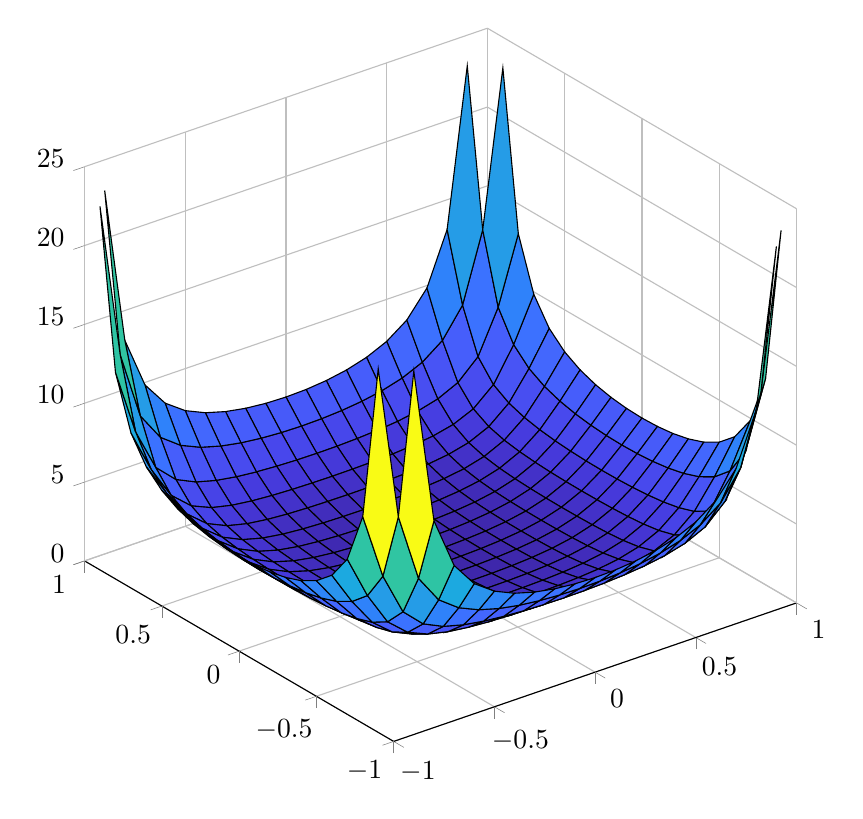
\begin{tikzpicture}

\begin{axis}[%
width=3.56in,
height=3.566in,
at={(0.597in,0.481in)},
scale only axis,
unbounded coords=jump,
xmin=-1,
xmax=1,
tick align=outside,
ymin=-1,
ymax=1,
zmin=0,
zmax=25,
view={-37.5}{30},
axis background/.style={fill=white},
axis x line*=bottom,
axis y line*=left,
axis z line*=left,
xmajorgrids,
ymajorgrids,
zmajorgrids,
legend style={at={(1.03,1)}, anchor=north west, legend cell align=left, align=left, draw=white!15!black}
]

\addplot3[%
surf,
shader=flat corner, draw=black, z buffer=sort, colormap={mymap}{[1pt] rgb(0pt)=(0.2422,0.1504,0.6603); rgb(1pt)=(0.25039,0.164995,0.707614); rgb(2pt)=(0.257771,0.181781,0.751138); rgb(3pt)=(0.264729,0.197757,0.795214); rgb(4pt)=(0.270648,0.214676,0.836371); rgb(5pt)=(0.275114,0.234238,0.870986); rgb(6pt)=(0.2783,0.255871,0.899071); rgb(7pt)=(0.280333,0.278233,0.9221); rgb(8pt)=(0.281338,0.300595,0.941376); rgb(9pt)=(0.281014,0.322757,0.957886); rgb(10pt)=(0.279467,0.344671,0.971676); rgb(11pt)=(0.275971,0.366681,0.982905); rgb(12pt)=(0.269914,0.3892,0.9906); rgb(13pt)=(0.260243,0.412329,0.995157); rgb(14pt)=(0.244033,0.435833,0.998833); rgb(15pt)=(0.220643,0.460257,0.997286); rgb(16pt)=(0.196333,0.484719,0.989152); rgb(17pt)=(0.183405,0.507371,0.979795); rgb(18pt)=(0.178643,0.528857,0.968157); rgb(19pt)=(0.176438,0.549905,0.952019); rgb(20pt)=(0.168743,0.570262,0.935871); rgb(21pt)=(0.154,0.5902,0.9218); rgb(22pt)=(0.146029,0.609119,0.907857); rgb(23pt)=(0.138024,0.627629,0.89729); rgb(24pt)=(0.124814,0.645929,0.888343); rgb(25pt)=(0.111252,0.6635,0.876314); rgb(26pt)=(0.0952095,0.679829,0.859781); rgb(27pt)=(0.0688714,0.694771,0.839357); rgb(28pt)=(0.0296667,0.708167,0.816333); rgb(29pt)=(0.00357143,0.720267,0.7917); rgb(30pt)=(0.00665714,0.731214,0.766014); rgb(31pt)=(0.0433286,0.741095,0.73941); rgb(32pt)=(0.0963952,0.75,0.712038); rgb(33pt)=(0.140771,0.7584,0.684157); rgb(34pt)=(0.1717,0.766962,0.655443); rgb(35pt)=(0.193767,0.775767,0.6251); rgb(36pt)=(0.216086,0.7843,0.5923); rgb(37pt)=(0.246957,0.791795,0.556743); rgb(38pt)=(0.290614,0.79729,0.518829); rgb(39pt)=(0.340643,0.8008,0.478857); rgb(40pt)=(0.3909,0.802871,0.435448); rgb(41pt)=(0.445629,0.802419,0.390919); rgb(42pt)=(0.5044,0.7993,0.348); rgb(43pt)=(0.561562,0.794233,0.304481); rgb(44pt)=(0.617395,0.787619,0.261238); rgb(45pt)=(0.671986,0.779271,0.2227); rgb(46pt)=(0.7242,0.769843,0.191029); rgb(47pt)=(0.773833,0.759805,0.16461); rgb(48pt)=(0.820314,0.749814,0.153529); rgb(49pt)=(0.863433,0.7406,0.159633); rgb(50pt)=(0.903543,0.733029,0.177414); rgb(51pt)=(0.939257,0.728786,0.209957); rgb(52pt)=(0.972757,0.729771,0.239443); rgb(53pt)=(0.995648,0.743371,0.237148); rgb(54pt)=(0.996986,0.765857,0.219943); rgb(55pt)=(0.995205,0.789252,0.202762); rgb(56pt)=(0.9892,0.813567,0.188533); rgb(57pt)=(0.978629,0.838629,0.176557); rgb(58pt)=(0.967648,0.8639,0.16429); rgb(59pt)=(0.96101,0.889019,0.153676); rgb(60pt)=(0.959671,0.913457,0.142257); rgb(61pt)=(0.962795,0.937338,0.12651); rgb(62pt)=(0.969114,0.960629,0.106362); rgb(63pt)=(0.9769,0.9839,0.0805)}, mesh/rows=21]
table[row sep=crcr, point meta=\thisrow{c}] {%
%
x	y	z	c\\
-1	-1	nan	nan\\
-1	-0.9	23.0526315789476	23.0526315789476\\
-1	-0.8	13.111111111111	13.111111111111\\
-1	-0.7	9.84313725490198	9.84313725490198\\
-1	-0.6	8.25	8.25\\
-1	-0.5	7.33333333333333	7.33333333333333\\
-1	-0.4	6.76190476190476	6.76190476190476\\
-1	-0.3	6.3956043956044	6.3956043956044\\
-1	-0.2	6.16666666666667	6.16666666666667\\
-1	-0.1	6.04040404040404	6.04040404040404\\
-1	0	6	6\\
-1	0.1	6.04040404040404	6.04040404040404\\
-1	0.2	6.16666666666667	6.16666666666667\\
-1	0.3	6.3956043956044	6.3956043956044\\
-1	0.4	6.76190476190476	6.76190476190476\\
-1	0.5	7.33333333333333	7.33333333333333\\
-1	0.6	8.25	8.25\\
-1	0.7	9.84313725490198	9.84313725490198\\
-1	0.8	13.111111111111	13.111111111111\\
-1	0.9	23.0526315789476	23.0526315789476\\
-1	1	nan	nan\\
-0.9	-1	23.0526315789474	23.0526315789474\\
-0.9	-0.9	13.2296043018034	13.2296043018034\\
-0.9	-0.8	8.89323388448234	8.89323388448234\\
-0.9	-0.7	7.09420343222335	7.09420343222335\\
-0.9	-0.6	6.14827799579131	6.14827799579131\\
-0.9	-0.5	5.58320204291365	5.58320204291365\\
-0.9	-0.4	5.22320986422556	5.22320986422556\\
-0.9	-0.3	4.98931926341663	4.98931926341663\\
-0.9	-0.2	4.8418995803402	4.8418995803402\\
-0.9	-0.1	4.76018879898449	4.76018879898449\\
-0.9	0	4.73398039226131	4.73398039226131\\
-0.9	0.1	4.76018879898449	4.76018879898449\\
-0.9	0.2	4.8418995803402	4.8418995803402\\
-0.9	0.3	4.98931926341663	4.98931926341663\\
-0.9	0.4	5.22320986422556	5.22320986422556\\
-0.9	0.5	5.58320204291365	5.58320204291365\\
-0.9	0.6	6.14827799579131	6.14827799579131\\
-0.9	0.7	7.09420343222335	7.09420343222335\\
-0.9	0.8	8.89323388448234	8.89323388448234\\
-0.9	0.9	13.2296043018034	13.2296043018034\\
-0.9	1	23.0526315789474	23.0526315789474\\
-0.8	-1	13.1111111111111	13.1111111111111\\
-0.8	-0.9	8.89323388448241	8.89323388448241\\
-0.8	-0.8	6.19988776369148	6.19988776369148\\
-0.8	-0.7	4.9939165246783	4.9939165246783\\
-0.8	-0.6	4.39602375110444	4.39602375110444\\
-0.8	-0.5	4.05755366965927	4.05755366965927\\
-0.8	-0.4	3.84907306567848	3.84907306567848\\
-0.8	-0.3	3.71621993056871	3.71621993056871\\
-0.8	-0.2	3.63337795901121	3.63337795901121\\
-0.8	-0.1	3.58771872965006	3.58771872965006\\
-0.8	0	3.57310898616177	3.57310898616177\\
-0.8	0.1	3.58771872965006	3.58771872965006\\
-0.8	0.2	3.63337795901121	3.63337795901121\\
-0.8	0.3	3.71621993056871	3.71621993056871\\
-0.8	0.4	3.84907306567848	3.84907306567848\\
-0.8	0.5	4.05755366965927	4.05755366965927\\
-0.8	0.6	4.39602375110444	4.39602375110444\\
-0.8	0.7	4.9939165246783	4.9939165246783\\
-0.8	0.8	6.19988776369148	6.19988776369148\\
-0.8	0.9	8.89323388448241	8.89323388448241\\
-0.8	1	13.1111111111111	13.1111111111111\\
-0.7	-1	9.84313725490198	9.84313725490198\\
-0.7	-0.9	7.09420343222336	7.09420343222336\\
-0.7	-0.8	4.99391652467831	4.99391652467831\\
-0.7	-0.7	3.88908128922564	3.88908128922564\\
-0.7	-0.6	3.33774331277907	3.33774331277907\\
-0.7	-0.5	3.04788249518098	3.04788249518098\\
-0.7	-0.4	2.88518758693567	2.88518758693567\\
-0.7	-0.3	2.78981199902195	2.78981199902195\\
-0.7	-0.2	2.73402424622654	2.73402424622654\\
-0.7	-0.1	2.70454808009259	2.70454808009259\\
-0.7	0	2.69531099391084	2.69531099391084\\
-0.7	0.1	2.70454808009259	2.70454808009259\\
-0.7	0.2	2.73402424622654	2.73402424622654\\
-0.7	0.3	2.78981199902195	2.78981199902195\\
-0.7	0.4	2.88518758693567	2.88518758693567\\
-0.7	0.5	3.04788249518098	3.04788249518098\\
-0.7	0.6	3.33774331277907	3.33774331277907\\
-0.7	0.7	3.88908128922564	3.88908128922564\\
-0.7	0.8	4.99391652467831	4.99391652467831\\
-0.7	0.9	7.09420343222336	7.09420343222336\\
-0.7	1	9.84313725490198	9.84313725490198\\
-0.6	-1	8.24999999999999	8.24999999999999\\
-0.6	-0.9	6.14827799579132	6.14827799579132\\
-0.6	-0.8	4.39602375110444	4.39602375110444\\
-0.6	-0.7	3.33774331277907	3.33774331277907\\
-0.6	-0.6	2.76256313292354	2.76256313292354\\
-0.6	-0.5	2.45286827306655	2.45286827306655\\
-0.6	-0.4	2.28240657625557	2.28240657625557\\
-0.6	-0.3	2.18662860979927	2.18662860979927\\
-0.6	-0.2	2.13322049347278	2.13322049347278\\
-0.6	-0.1	2.10609862401655	2.10609862401655\\
-0.6	0	2.09778596995664	2.09778596995664\\
-0.6	0.1	2.10609862401655	2.10609862401655\\
-0.6	0.2	2.13322049347278	2.13322049347278\\
-0.6	0.3	2.18662860979927	2.18662860979927\\
-0.6	0.4	2.28240657625557	2.28240657625557\\
-0.6	0.5	2.45286827306655	2.45286827306655\\
-0.6	0.6	2.76256313292354	2.76256313292354\\
-0.6	0.7	3.33774331277907	3.33774331277907\\
-0.6	0.8	4.39602375110444	4.39602375110444\\
-0.6	0.9	6.14827799579132	6.14827799579132\\
-0.6	1	8.24999999999999	8.24999999999999\\
-0.5	-1	7.33333333333333	7.33333333333333\\
-0.5	-0.9	5.58320204291365	5.58320204291365\\
-0.5	-0.8	4.05755366965926	4.05755366965926\\
-0.5	-0.7	3.04788249518098	3.04788249518098\\
-0.5	-0.6	2.45286827306655	2.45286827306655\\
-0.5	-0.5	2.11438191683587	2.11438191683587\\
-0.5	-0.4	1.92230810937407	1.92230810937407\\
-0.5	-0.3	1.81309357845656	1.81309357845656\\
-0.5	-0.2	1.75218118209068	1.75218118209068\\
-0.5	-0.1	1.72139668275897	1.72139668275897\\
-0.5	0	1.712	1.712\\
-0.5	0.1	1.72139668275897	1.72139668275897\\
-0.5	0.2	1.75218118209068	1.75218118209068\\
-0.5	0.3	1.81309357845656	1.81309357845656\\
-0.5	0.4	1.92230810937407	1.92230810937407\\
-0.5	0.5	2.11438191683587	2.11438191683587\\
-0.5	0.6	2.45286827306655	2.45286827306655\\
-0.5	0.7	3.04788249518098	3.04788249518098\\
-0.5	0.8	4.05755366965926	4.05755366965926\\
-0.5	0.9	5.58320204291365	5.58320204291365\\
-0.5	1	7.33333333333333	7.33333333333333\\
-0.4	-1	6.76190476190476	6.76190476190476\\
-0.4	-0.9	5.22320986422556	5.22320986422556\\
-0.4	-0.8	3.84907306567848	3.84907306567848\\
-0.4	-0.7	2.88518758693567	2.88518758693567\\
-0.4	-0.6	2.28240657625558	2.28240657625558\\
-0.4	-0.5	1.92230810937407	1.92230810937407\\
-0.4	-0.4	1.71032089901499	1.71032089901499\\
-0.4	-0.3	1.58660034951018	1.58660034951018\\
-0.4	-0.2	1.51638590795481	1.51638590795481\\
-0.4	-0.1	1.48052510090217	1.48052510090217\\
-0.4	0	1.46952499618196	1.46952499618196\\
-0.4	0.1	1.48052510090217	1.48052510090217\\
-0.4	0.2	1.51638590795481	1.51638590795481\\
-0.4	0.3	1.58660034951018	1.58660034951018\\
-0.4	0.4	1.71032089901499	1.71032089901499\\
-0.4	0.5	1.92230810937407	1.92230810937407\\
-0.4	0.6	2.28240657625558	2.28240657625558\\
-0.4	0.7	2.88518758693567	2.88518758693567\\
-0.4	0.8	3.84907306567848	3.84907306567848\\
-0.4	0.9	5.22320986422556	5.22320986422556\\
-0.4	1	6.76190476190476	6.76190476190476\\
-0.3	-1	6.3956043956044	6.3956043956044\\
-0.3	-0.9	4.98931926341663	4.98931926341663\\
-0.3	-0.8	3.71621993056871	3.71621993056871\\
-0.3	-0.7	2.78981199902195	2.78981199902195\\
-0.3	-0.6	2.18662860979928	2.18662860979928\\
-0.3	-0.5	1.81309357845656	1.81309357845656\\
-0.3	-0.4	1.58660034951018	1.58660034951018\\
-0.3	-0.3	1.45130742605288	1.45130742605288\\
-0.3	-0.2	1.3731816152005	1.3731816152005\\
-0.3	-0.1	1.33281170445424	1.33281170445424\\
-0.3	0	1.32035502909706	1.32035502909706\\
-0.3	0.1	1.33281170445424	1.33281170445424\\
-0.3	0.2	1.3731816152005	1.3731816152005\\
-0.3	0.3	1.45130742605288	1.45130742605288\\
-0.3	0.4	1.58660034951018	1.58660034951018\\
-0.3	0.5	1.81309357845656	1.81309357845656\\
-0.3	0.6	2.18662860979928	2.18662860979928\\
-0.3	0.7	2.78981199902195	2.78981199902195\\
-0.3	0.8	3.71621993056871	3.71621993056871\\
-0.3	0.9	4.98931926341663	4.98931926341663\\
-0.3	1	6.3956043956044	6.3956043956044\\
-0.2	-1	6.16666666666667	6.16666666666667\\
-0.2	-0.9	4.8418995803402	4.8418995803402\\
-0.2	-0.8	3.63337795901121	3.63337795901121\\
-0.2	-0.7	2.73402424622654	2.73402424622654\\
-0.2	-0.6	2.13322049347279	2.13322049347279\\
-0.2	-0.5	1.75218118209068	1.75218118209068\\
-0.2	-0.4	1.51638590795481	1.51638590795481\\
-0.2	-0.3	1.37318161520051	1.37318161520051\\
-0.2	-0.2	1.28942400545157	1.28942400545157\\
-0.2	-0.1	1.24576115741349	1.24576115741349\\
-0.2	0	1.23222725701503	1.23222725701503\\
-0.2	0.1	1.24576115741349	1.24576115741349\\
-0.2	0.2	1.28942400545157	1.28942400545157\\
-0.2	0.3	1.37318161520051	1.37318161520051\\
-0.2	0.4	1.51638590795481	1.51638590795481\\
-0.2	0.5	1.75218118209068	1.75218118209068\\
-0.2	0.6	2.13322049347279	2.13322049347279\\
-0.2	0.7	2.73402424622654	2.73402424622654\\
-0.2	0.8	3.63337795901121	3.63337795901121\\
-0.2	0.9	4.8418995803402	4.8418995803402\\
-0.2	1	6.16666666666667	6.16666666666667\\
-0.1	-1	6.04040404040404	6.04040404040404\\
-0.1	-0.9	4.76018879898449	4.76018879898449\\
-0.1	-0.8	3.58771872965006	3.58771872965006\\
-0.1	-0.7	2.70454808009259	2.70454808009259\\
-0.1	-0.6	2.10609862401655	2.10609862401655\\
-0.1	-0.5	1.72139668275897	1.72139668275897\\
-0.1	-0.4	1.48052510090217	1.48052510090217\\
-0.1	-0.3	1.33281170445424	1.33281170445424\\
-0.1	-0.2	1.24576115741349	1.24576115741349\\
-0.1	-0.1	1.20014284621084	1.20014284621084\\
-0.1	0	1.1859644491566	1.1859644491566\\
-0.1	0.1	1.20014284621084	1.20014284621084\\
-0.1	0.2	1.24576115741349	1.24576115741349\\
-0.1	0.3	1.33281170445424	1.33281170445424\\
-0.1	0.4	1.48052510090217	1.48052510090217\\
-0.1	0.5	1.72139668275897	1.72139668275897\\
-0.1	0.6	2.10609862401655	2.10609862401655\\
-0.1	0.7	2.70454808009259	2.70454808009259\\
-0.1	0.8	3.58771872965006	3.58771872965006\\
-0.1	0.9	4.76018879898449	4.76018879898449\\
-0.1	1	6.04040404040404	6.04040404040404\\
0	-1	6	6\\
0	-0.9	4.73398039226131	4.73398039226131\\
0	-0.8	3.57310898616177	3.57310898616177\\
0	-0.7	2.69531099391084	2.69531099391084\\
0	-0.6	2.09778596995664	2.09778596995664\\
0	-0.5	1.712	1.712\\
0	-0.4	1.46952499618196	1.46952499618196\\
0	-0.3	1.32035502909706	1.32035502909706\\
0	-0.2	1.23222725701503	1.23222725701503\\
0	-0.1	1.1859644491566	1.1859644491566\\
0	0	1.17157287525381	1.17157287525381\\
0	0.1	1.1859644491566	1.1859644491566\\
0	0.2	1.23222725701503	1.23222725701503\\
0	0.3	1.32035502909706	1.32035502909706\\
0	0.4	1.46952499618196	1.46952499618196\\
0	0.5	1.712	1.712\\
0	0.6	2.09778596995664	2.09778596995664\\
0	0.7	2.69531099391084	2.69531099391084\\
0	0.8	3.57310898616177	3.57310898616177\\
0	0.9	4.73398039226131	4.73398039226131\\
0	1	6	6\\
0.1	-1	6.04040404040404	6.04040404040404\\
0.1	-0.9	4.76018879898449	4.76018879898449\\
0.1	-0.8	3.58771872965006	3.58771872965006\\
0.1	-0.7	2.70454808009259	2.70454808009259\\
0.1	-0.6	2.10609862401655	2.10609862401655\\
0.1	-0.5	1.72139668275897	1.72139668275897\\
0.1	-0.4	1.48052510090217	1.48052510090217\\
0.1	-0.3	1.33281170445424	1.33281170445424\\
0.1	-0.2	1.24576115741349	1.24576115741349\\
0.1	-0.1	1.20014284621084	1.20014284621084\\
0.1	0	1.1859644491566	1.1859644491566\\
0.1	0.1	1.20014284621084	1.20014284621084\\
0.1	0.2	1.24576115741349	1.24576115741349\\
0.1	0.3	1.33281170445424	1.33281170445424\\
0.1	0.4	1.48052510090217	1.48052510090217\\
0.1	0.5	1.72139668275897	1.72139668275897\\
0.1	0.6	2.10609862401655	2.10609862401655\\
0.1	0.7	2.70454808009259	2.70454808009259\\
0.1	0.8	3.58771872965006	3.58771872965006\\
0.1	0.9	4.76018879898449	4.76018879898449\\
0.1	1	6.04040404040404	6.04040404040404\\
0.2	-1	6.16666666666667	6.16666666666667\\
0.2	-0.9	4.8418995803402	4.8418995803402\\
0.2	-0.8	3.63337795901121	3.63337795901121\\
0.2	-0.7	2.73402424622654	2.73402424622654\\
0.2	-0.6	2.13322049347279	2.13322049347279\\
0.2	-0.5	1.75218118209068	1.75218118209068\\
0.2	-0.4	1.51638590795481	1.51638590795481\\
0.2	-0.3	1.37318161520051	1.37318161520051\\
0.2	-0.2	1.28942400545157	1.28942400545157\\
0.2	-0.1	1.24576115741349	1.24576115741349\\
0.2	0	1.23222725701503	1.23222725701503\\
0.2	0.1	1.24576115741349	1.24576115741349\\
0.2	0.2	1.28942400545157	1.28942400545157\\
0.2	0.3	1.37318161520051	1.37318161520051\\
0.2	0.4	1.51638590795481	1.51638590795481\\
0.2	0.5	1.75218118209068	1.75218118209068\\
0.2	0.6	2.13322049347279	2.13322049347279\\
0.2	0.7	2.73402424622654	2.73402424622654\\
0.2	0.8	3.63337795901121	3.63337795901121\\
0.2	0.9	4.8418995803402	4.8418995803402\\
0.2	1	6.16666666666667	6.16666666666667\\
0.3	-1	6.3956043956044	6.3956043956044\\
0.3	-0.9	4.98931926341663	4.98931926341663\\
0.3	-0.8	3.71621993056871	3.71621993056871\\
0.3	-0.7	2.78981199902195	2.78981199902195\\
0.3	-0.6	2.18662860979928	2.18662860979928\\
0.3	-0.5	1.81309357845656	1.81309357845656\\
0.3	-0.4	1.58660034951018	1.58660034951018\\
0.3	-0.3	1.45130742605288	1.45130742605288\\
0.3	-0.2	1.3731816152005	1.3731816152005\\
0.3	-0.1	1.33281170445424	1.33281170445424\\
0.3	0	1.32035502909706	1.32035502909706\\
0.3	0.1	1.33281170445424	1.33281170445424\\
0.3	0.2	1.3731816152005	1.3731816152005\\
0.3	0.3	1.45130742605288	1.45130742605288\\
0.3	0.4	1.58660034951018	1.58660034951018\\
0.3	0.5	1.81309357845656	1.81309357845656\\
0.3	0.6	2.18662860979928	2.18662860979928\\
0.3	0.7	2.78981199902195	2.78981199902195\\
0.3	0.8	3.71621993056871	3.71621993056871\\
0.3	0.9	4.98931926341663	4.98931926341663\\
0.3	1	6.3956043956044	6.3956043956044\\
0.4	-1	6.76190476190476	6.76190476190476\\
0.4	-0.9	5.22320986422556	5.22320986422556\\
0.4	-0.8	3.84907306567848	3.84907306567848\\
0.4	-0.7	2.88518758693567	2.88518758693567\\
0.4	-0.6	2.28240657625558	2.28240657625558\\
0.4	-0.5	1.92230810937407	1.92230810937407\\
0.4	-0.4	1.71032089901499	1.71032089901499\\
0.4	-0.3	1.58660034951018	1.58660034951018\\
0.4	-0.2	1.51638590795481	1.51638590795481\\
0.4	-0.1	1.48052510090217	1.48052510090217\\
0.4	0	1.46952499618196	1.46952499618196\\
0.4	0.1	1.48052510090217	1.48052510090217\\
0.4	0.2	1.51638590795481	1.51638590795481\\
0.4	0.3	1.58660034951018	1.58660034951018\\
0.4	0.4	1.71032089901499	1.71032089901499\\
0.4	0.5	1.92230810937407	1.92230810937407\\
0.4	0.6	2.28240657625558	2.28240657625558\\
0.4	0.7	2.88518758693567	2.88518758693567\\
0.4	0.8	3.84907306567848	3.84907306567848\\
0.4	0.9	5.22320986422556	5.22320986422556\\
0.4	1	6.76190476190476	6.76190476190476\\
0.5	-1	7.33333333333333	7.33333333333333\\
0.5	-0.9	5.58320204291365	5.58320204291365\\
0.5	-0.8	4.05755366965926	4.05755366965926\\
0.5	-0.7	3.04788249518098	3.04788249518098\\
0.5	-0.6	2.45286827306655	2.45286827306655\\
0.5	-0.5	2.11438191683587	2.11438191683587\\
0.5	-0.4	1.92230810937407	1.92230810937407\\
0.5	-0.3	1.81309357845656	1.81309357845656\\
0.5	-0.2	1.75218118209068	1.75218118209068\\
0.5	-0.1	1.72139668275897	1.72139668275897\\
0.5	0	1.712	1.712\\
0.5	0.1	1.72139668275897	1.72139668275897\\
0.5	0.2	1.75218118209068	1.75218118209068\\
0.5	0.3	1.81309357845656	1.81309357845656\\
0.5	0.4	1.92230810937407	1.92230810937407\\
0.5	0.5	2.11438191683587	2.11438191683587\\
0.5	0.6	2.45286827306655	2.45286827306655\\
0.5	0.7	3.04788249518098	3.04788249518098\\
0.5	0.8	4.05755366965926	4.05755366965926\\
0.5	0.9	5.58320204291365	5.58320204291365\\
0.5	1	7.33333333333333	7.33333333333333\\
0.6	-1	8.24999999999999	8.24999999999999\\
0.6	-0.9	6.14827799579132	6.14827799579132\\
0.6	-0.8	4.39602375110444	4.39602375110444\\
0.6	-0.7	3.33774331277907	3.33774331277907\\
0.6	-0.6	2.76256313292354	2.76256313292354\\
0.6	-0.5	2.45286827306655	2.45286827306655\\
0.6	-0.4	2.28240657625557	2.28240657625557\\
0.6	-0.3	2.18662860979927	2.18662860979927\\
0.6	-0.2	2.13322049347278	2.13322049347278\\
0.6	-0.1	2.10609862401655	2.10609862401655\\
0.6	0	2.09778596995664	2.09778596995664\\
0.6	0.1	2.10609862401655	2.10609862401655\\
0.6	0.2	2.13322049347278	2.13322049347278\\
0.6	0.3	2.18662860979927	2.18662860979927\\
0.6	0.4	2.28240657625557	2.28240657625557\\
0.6	0.5	2.45286827306655	2.45286827306655\\
0.6	0.6	2.76256313292354	2.76256313292354\\
0.6	0.7	3.33774331277907	3.33774331277907\\
0.6	0.8	4.39602375110444	4.39602375110444\\
0.6	0.9	6.14827799579132	6.14827799579132\\
0.6	1	8.24999999999999	8.24999999999999\\
0.7	-1	9.84313725490198	9.84313725490198\\
0.7	-0.9	7.09420343222336	7.09420343222336\\
0.7	-0.8	4.99391652467831	4.99391652467831\\
0.7	-0.7	3.88908128922564	3.88908128922564\\
0.7	-0.6	3.33774331277907	3.33774331277907\\
0.7	-0.5	3.04788249518098	3.04788249518098\\
0.7	-0.4	2.88518758693567	2.88518758693567\\
0.7	-0.3	2.78981199902195	2.78981199902195\\
0.7	-0.2	2.73402424622654	2.73402424622654\\
0.7	-0.1	2.70454808009259	2.70454808009259\\
0.7	0	2.69531099391084	2.69531099391084\\
0.7	0.1	2.70454808009259	2.70454808009259\\
0.7	0.2	2.73402424622654	2.73402424622654\\
0.7	0.3	2.78981199902195	2.78981199902195\\
0.7	0.4	2.88518758693567	2.88518758693567\\
0.7	0.5	3.04788249518098	3.04788249518098\\
0.7	0.6	3.33774331277907	3.33774331277907\\
0.7	0.7	3.88908128922564	3.88908128922564\\
0.7	0.8	4.99391652467831	4.99391652467831\\
0.7	0.9	7.09420343222336	7.09420343222336\\
0.7	1	9.84313725490198	9.84313725490198\\
0.8	-1	13.1111111111111	13.1111111111111\\
0.8	-0.9	8.89323388448241	8.89323388448241\\
0.8	-0.8	6.19988776369148	6.19988776369148\\
0.8	-0.7	4.9939165246783	4.9939165246783\\
0.8	-0.6	4.39602375110444	4.39602375110444\\
0.8	-0.5	4.05755366965927	4.05755366965927\\
0.8	-0.4	3.84907306567848	3.84907306567848\\
0.8	-0.3	3.71621993056871	3.71621993056871\\
0.8	-0.2	3.63337795901121	3.63337795901121\\
0.8	-0.1	3.58771872965006	3.58771872965006\\
0.8	0	3.57310898616177	3.57310898616177\\
0.8	0.1	3.58771872965006	3.58771872965006\\
0.8	0.2	3.63337795901121	3.63337795901121\\
0.8	0.3	3.71621993056871	3.71621993056871\\
0.8	0.4	3.84907306567848	3.84907306567848\\
0.8	0.5	4.05755366965927	4.05755366965927\\
0.8	0.6	4.39602375110444	4.39602375110444\\
0.8	0.7	4.9939165246783	4.9939165246783\\
0.8	0.8	6.19988776369148	6.19988776369148\\
0.8	0.9	8.89323388448241	8.89323388448241\\
0.8	1	13.1111111111111	13.1111111111111\\
0.9	-1	23.0526315789474	23.0526315789474\\
0.9	-0.9	13.2296043018034	13.2296043018034\\
0.9	-0.8	8.89323388448234	8.89323388448234\\
0.9	-0.7	7.09420343222335	7.09420343222335\\
0.9	-0.6	6.14827799579131	6.14827799579131\\
0.9	-0.5	5.58320204291365	5.58320204291365\\
0.9	-0.4	5.22320986422556	5.22320986422556\\
0.9	-0.3	4.98931926341663	4.98931926341663\\
0.9	-0.2	4.8418995803402	4.8418995803402\\
0.9	-0.1	4.76018879898449	4.76018879898449\\
0.9	0	4.73398039226131	4.73398039226131\\
0.9	0.1	4.76018879898449	4.76018879898449\\
0.9	0.2	4.8418995803402	4.8418995803402\\
0.9	0.3	4.98931926341663	4.98931926341663\\
0.9	0.4	5.22320986422556	5.22320986422556\\
0.9	0.5	5.58320204291365	5.58320204291365\\
0.9	0.6	6.14827799579131	6.14827799579131\\
0.9	0.7	7.09420343222335	7.09420343222335\\
0.9	0.8	8.89323388448234	8.89323388448234\\
0.9	0.9	13.2296043018034	13.2296043018034\\
0.9	1	23.0526315789474	23.0526315789474\\
1	-1	nan	nan\\
1	-0.9	23.0526315789476	23.0526315789476\\
1	-0.8	13.111111111111	13.111111111111\\
1	-0.7	9.84313725490198	9.84313725490198\\
1	-0.6	8.25	8.25\\
1	-0.5	7.33333333333333	7.33333333333333\\
1	-0.4	6.76190476190476	6.76190476190476\\
1	-0.3	6.3956043956044	6.3956043956044\\
1	-0.2	6.16666666666667	6.16666666666667\\
1	-0.1	6.04040404040404	6.04040404040404\\
1	0	6	6\\
1	0.1	6.04040404040404	6.04040404040404\\
1	0.2	6.16666666666667	6.16666666666667\\
1	0.3	6.3956043956044	6.3956043956044\\
1	0.4	6.76190476190476	6.76190476190476\\
1	0.5	7.33333333333333	7.33333333333333\\
1	0.6	8.25	8.25\\
1	0.7	9.84313725490198	9.84313725490198\\
1	0.8	13.111111111111	13.111111111111\\
1	0.9	23.0526315789476	23.0526315789476\\
1	1	nan	nan\\
};
%\addlegendentry{data1}

\end{axis}
\end{tikzpicture}%
}
\caption{Negativer Laplace der Gewichtsfunktion}
\label{fig:Gewicht}
\end{figure}
\subsubsection{Zufällige Kollokationspunkte}
Als nächstes schauen wir uns zufällig verteilte Kollokationspunkte an. In Abbildung \ref{fig:error-random} ist der Fehler bei unterschiedlich vielen zufällig verteilten Kollokationspunkten dargestellt.
\begin{figure}[ht]
\centering
\resizebox {\columnwidth} {!} {
% This file was created by matlab2tikz.
%
%The latest updates can be retrieved from
%  http://www.mathworks.com/matlabcentral/fileexchange/22022-matlab2tikz-matlab2tikz
%where you can also make suggestions and rate matlab2tikz.
%
\definecolor{mycolor1}{rgb}{0.00000,0.44700,0.74100}%
\definecolor{mycolor2}{rgb}{0.85000,0.32500,0.09800}%
\definecolor{mycolor3}{rgb}{0.92900,0.69400,0.12500}%
\definecolor{mycolor4}{rgb}{0.49400,0.18400,0.55600}%
%
\begin{tikzpicture}

\begin{axis}[%
width=4.521in,
height=3.566in,
at={(0.758in,0.481in)},
scale only axis,
xmin=0,
xmax=3000,
xlabel style={font=\color{white!15!black}},
xlabel={Anzahl der Kollokationspunkte},
ymode=log,
ymin=1e-08,
ymax=1,
yminorticks=true,
ylabel style={font=\color{white!15!black}},
ylabel={Maximaler absoluter Fehler},
axis background/.style={fill=white},
%title style={font=\bfseries},
%title={error plot},
legend style={legend cell align=left, align=left, draw=white!15!black}
]
\addplot [color=mycolor1]
  table[row sep=crcr]{%
4	0.999748271191593\\
8	1.08133089295795\\
17	0.787488457043724\\
28	1.00876021033637\\
41	0.0527639218376913\\
56	0.0109041187286126\\
73	0.00406914619466443\\
92	0.000718967326502562\\
113	7.14934437407964e-05\\
136	1.0394229939939e-05\\
161	4.05968459937789e-05\\
188	1.59883979566899e-06\\
217	2.10279376054723e-06\\
248	7.56134738222336e-06\\
281	0.000153039106389988\\
316	7.55029009213981e-06\\
353	5.91196770269309e-06\\
392	4.59954539053925e-06\\
433	2.53142893736902e-05\\
476	1.4072184219005e-06\\
521	9.0805385786763e-06\\
568	7.02877939401381e-06\\
617	9.65326440827141e-06\\
668	6.53233612457615e-06\\
721	7.71608473371099e-06\\
776	4.47640278899986e-06\\
833	9.75911040312916e-07\\
892	2.536628800065e-06\\
953	1.03296259561514e-05\\
1016	4.49691019682036e-06\\
1081	5.79796909065677e-06\\
1148	5.36176315985015e-07\\
1217	6.67522949859833e-07\\
1288	5.7846619649915e-07\\
1361	1.02039667068676e-06\\
1436	2.01015942932758e-05\\
1513	1.49408012528607e-06\\
1592	1.53918436382461e-06\\
1673	4.58170527043722e-05\\
1756	9.44525468289659e-07\\
1841	3.6672603868082e-06\\
1928	8.21270517814554e-07\\
2017	5.44312765882182e-06\\
2108	2.58230115202096e-06\\
2201	1.30267089670788e-06\\
2296	9.10570958706503e-06\\
2393	2.30663158780342e-06\\
2492	1.63296681199299e-06\\
2593	1.28691629730504e-06\\
2696	2.50154829639637e-06\\
2801	3.03184176456139e-06\\
2908	3.54799379120863e-06\\
3017	4.79236326328715e-05\\
%3128	6.02316715461737e-06\\
%3241	1.7150268772359e-06\\
};
\addlegendentry{Standard N-Sym}

\addplot [color=mycolor2]
  table[row sep=crcr]{%
4	1.05433617432393\\
8	1.00032665947363\\
17	0.656244606477592\\
28	0.488123125287577\\
41	0.0167595794262468\\
56	0.0126425780735455\\
73	0.00176754336468821\\
92	0.000367559673635359\\
113	4.29232002490121e-05\\
136	4.42396413366519e-06\\
161	1.15774510173888e-06\\
188	1.37540730423685e-06\\
217	1.31405627492309e-05\\
248	2.4364927175835e-07\\
281	2.91152883069579e-06\\
316	4.04687917843205e-07\\
353	2.56703371314879e-07\\
392	4.61335609117097e-07\\
433	1.50778136864815e-07\\
476	3.88877087864614e-07\\
521	1.73850616269622e-06\\
568	1.86488130382578e-07\\
617	2.16339936420784e-06\\
668	1.75947158773115e-07\\
721	1.11544479042269e-07\\
776	2.07809496832745e-07\\
833	7.25611153162831e-07\\
892	6.27616288162436e-07\\
953	2.748787992779e-07\\
1016	4.25056406849755e-07\\
1081	4.95227150620892e-07\\
1148	6.60296271215444e-07\\
1217	3.6682225745821e-07\\
1288	6.01276105682835e-07\\
1361	2.35795907965741e-07\\
1436	9.30683431432655e-08\\
1513	2.39172673632826e-06\\
1592	3.42675820719229e-07\\
1673	9.38543386896917e-08\\
1756	2.5195072017592e-07\\
1841	5.76603644275586e-08\\
1928	7.46185584432624e-08\\
2017	1.35019466940278e-07\\
2108	1.8868877105227e-07\\
2201	1.48583618297948e-07\\
2296	5.29822003408897e-07\\
2393	3.40882660987418e-07\\
2492	5.04456426075883e-07\\
2593	2.10858148497195e-07\\
2696	7.93952114386265e-07\\
2801	1.4973639728133e-07\\
2908	8.17716342416119e-08\\
3017	6.1614441659863e-08\\
%3128	2.44505821644925e-07\\
%3241	2.26950638240742e-07\\
};
\addlegendentry{Standard Sym}

\addplot [color=mycolor3]
  table[row sep=crcr]{%
1	0.999748271191593\\
4	1.03142995437141\\
9	0.786116020859602\\
16	0.698872819735042\\
25	0.498915530291019\\
36	0.704722863175288\\
49	0.611470544068062\\
64	0.0106738238431806\\
81	0.00846406069694688\\
100	0.00742702542881313\\
121	0.0220102197149016\\
144	0.00457905440007705\\
169	0.00509467696278077\\
196	0.00703727304792809\\
225	0.00275120602099829\\
256	0.00441701737535992\\
289	0.00465806280572194\\
324	0.00276982772256065\\
361	0.0119481788398219\\
400	0.0013025263291274\\
441	0.00150669209981602\\
484	0.00217431067039899\\
529	0.00142201113861514\\
576	0.00221446456739976\\
625	0.00229094071132841\\
676	0.00119147529800234\\
729	0.000760281316827064\\
784	0.00103444806041601\\
841	0.0015600464205178\\
900	0.000626061907849821\\
961	0.00116075147651149\\
1024	0.000574065659955769\\
1089	0.0139310302097414\\
1156	0.00125073043455332\\
1225	0.000614581607711058\\
1296	0.000771687936694524\\
1369	0.0323749440009249\\
1444	0.000771991882251997\\
1521	0.000667891788862378\\
1600	0.00136046576912181\\
1681	0.000575470048991611\\
1764	0.000509889359674848\\
1849	0.000494766928465637\\
1936	0.000326558650546049\\
2025	0.00409080886488526\\
2116	0.000683812958245712\\
2209	0.00160371191726705\\
2304	0.000416075642606605\\
2401	0.000378952038433874\\
2500	0.000375028573406606\\
2601	0.000994625347152934\\
2704	0.000648966992822002\\
2809	0.000377421073108503\\
2916	0.000230095434709553\\
3025	0.000446172265639669\\
};
\addlegendentry{Gewichtet N-Sym}

\addplot [color=mycolor4]
  table[row sep=crcr]{%
1	0.999748271316304\\
4	0.999751384039337\\
9	0.909898599105437\\
16	0.620209403865854\\
25	0.0552234781086134\\
36	0.0362275171015879\\
49	0.0196258567645095\\
64	0.0216036616652308\\
81	0.0247118634926999\\
100	0.0125138003782383\\
121	0.00448730606378703\\
144	0.00939115922034597\\
169	0.00515212576558964\\
196	0.00894824020274193\\
225	0.0646436951925821\\
256	0.00196464535749688\\
289	0.00339906857097611\\
324	0.0021932638177733\\
361	0.0031423359427928\\
400	0.00237622812186326\\
441	0.00241798730992757\\
484	0.00237566816076224\\
529	0.00169974181119393\\
576	0.00162260594098848\\
625	0.00827509565468709\\
676	0.00201132129394521\\
729	0.00278213638848089\\
784	0.00322462890469077\\
841	0.000948345293616704\\
900	0.00499508125593828\\
961	0.000998783694139487\\
1024	0.00448608434440878\\
1089	0.000781102586880324\\
1156	0.00229222336556234\\
1225	0.00148211327985577\\
1296	0.000997588225633176\\
1369	0.000582902483207319\\
1444	0.000437834934091825\\
1521	0.00152806931504255\\
1600	0.000800994834489036\\
1681	0.000562049065303371\\
1764	0.000882555882422174\\
1849	0.000512296497525365\\
1936	0.00224544147747302\\
2025	0.000369847864830112\\
2116	0.0093295862010786\\
2209	0.000473890181991663\\
2304	0.00267560699936579\\
2401	0.000594623759577819\\
2500	0.000305277012374761\\
2601	0.000340357778171917\\
2704	0.000438210062154924\\
2809	0.000488154184416247\\
2916	0.00017351179575468\\
3025	0.000549801875980989\\
};
\addlegendentry{Gewichtet Sym}

\end{axis}
\end{tikzpicture}%
}
\caption{Fehler bei zufällig verteilten Kollokationspunkten}
\label{fig:error-random}
\end{figure}

Auch hier stellt man fest, dass alle Verfahren vernünftige Ergebnisse liefern. Die Standardverfahren erreichen mit $200$ Kollokationspunkten ihre besten Ergebnisse von rund $10^{-7}$ für die nicht-symmetrische Variante und $10^{-6}$ für die symmetrische und verbessern sich dann nicht mehr weiter. Die gewichteten Verfahren erreichen mit $200$ Kollokationspunkten nur einen Fehler von rund $10^{-2}$, verbessern sich aber mit mehr Kollokationspunkten noch leicht.

Vergleicht man die Fehler mit denen der Gitterpunktwahl, sieht man, dass diese sich in der gleichen Größenordnung bewegen. Allerdings weist die Kurve der zufällig gewählten Punkte mehrere Ausreißer nach oben auf. Diese sind auf eine zufällig schlechte Punktwahl zurückzuführen. Die zufälligen Punkte sind aber nie wesentlich besser als die Gitterpunkte. Von daher lässt sich in niedrigen Dimensionen kein Vorteil für zufällig gewählte Kollokationspunkte feststellen. In höheren Dimensionen ist es aufgrund der hohen Punktanzahl allerdings nahezu unmöglich ein Gitter über das Gebiet zu legen. Dort kann man dann davon ausgehen mit den zufällig gewählten Punkten vernünftige Ergebnisse zu erhalten.

\subsubsection{Greedy-Punktwahl}
Zuletzt schauen wir uns in Abbildung \ref{fig:error-greedy} mit einer Greedy-Punktwahl gesetzte Kollokationspunkte an. Es ist zu beachten, dass bei der benutzten Implementierung bei den Standardverfahren auf dem Rand festgesetzte Kollokationspunkte benutzt werden. Deswegen beginnen die Graphen der beiden Standardverfahren erst mit $37$ Kollokationspunkten.
\begin{figure}[ht]
\centering
\resizebox {\columnwidth} {!} {
% This file was created by matlab2tikz.
%
%The latest updates can be retrieved from
%  http://www.mathworks.com/matlabcentral/fileexchange/22022-matlab2tikz-matlab2tikz
%where you can also make suggestions and rate matlab2tikz.
%
\definecolor{mycolor1}{rgb}{0.00000,0.44700,0.74100}%
\definecolor{mycolor2}{rgb}{0.85000,0.32500,0.09800}%
\definecolor{mycolor3}{rgb}{0.92900,0.69400,0.12500}%
\definecolor{mycolor4}{rgb}{0.49400,0.18400,0.55600}%
%
\begin{tikzpicture}

\begin{axis}[%
width=4.521in,
height=3.566in,
at={(0.758in,0.481in)},
scale only axis,
xmin=0,
xmax=250,
xlabel style={font=\color{white!15!black}},
xlabel={Anzahl Kollokationspunkte},
ymode=log,
ymin=1e-08,
ymax=1.08072077358145,
yminorticks=true,
ylabel style={font=\color{white!15!black}},
ylabel={Maximaler absoluter Fehler},
axis background/.style={fill=white},
%title style={font=\bfseries},
%title={error plot},
legend style={legend cell align=left, align=left, draw=white!15!black},
legend pos = {south west}
]
\addplot [color=mycolor1]
  table[row sep=crcr]{%
37	0.998741611743565\\
38	1.56698113662613\\
39	1.42136798220903\\
40	0.0390994708809781\\
41	0.248340994602959\\
42	0.164178755435491\\
43	0.257088561832482\\
44	0.167554018875751\\
45	0.15029555458974\\
46	0.0398405178523725\\
47	0.0694103139259503\\
48	0.109226237003303\\
49	0.0660520350648076\\
50	0.0964940963117123\\
51	0.047066728058674\\
52	0.0436910549210606\\
53	0.0293446055808344\\
54	0.0211006316855517\\
55	0.0276976929175761\\
56	0.0211921990730971\\
57	0.0103875764832617\\
58	0.00722064148989227\\
59	0.0177039765776462\\
60	0.00575367368897617\\
61	0.0105342257537943\\
62	0.0107192608931312\\
63	0.00571232584370718\\
64	0.00747417551773089\\
65	0.00803971394621961\\
66	0.00217473435728519\\
67	0.000544432385404914\\
68	0.00212014655870951\\
69	0.00182510019522034\\
70	0.00238868533305021\\
71	0.0017977098497024\\
72	0.00313880426820937\\
73	0.00027769726807847\\
74	0.000199044228941125\\
75	0.000152182261049516\\
76	0.000213736913746099\\
77	0.000169367025339068\\
78	0.000114396474979274\\
79	0.000226111735248113\\
80	0.000391137412042775\\
81	7.48447510755534e-05\\
82	6.55505141003987e-05\\
83	5.16668725266678e-05\\
84	6.38462591333235e-05\\
85	5.29867437146364e-05\\
86	3.24099167953174e-05\\
87	2.8184817476018e-05\\
88	7.01514168349737e-05\\
89	5.38085245929132e-05\\
90	7.96424812544716e-05\\
91	4.61174110738538e-05\\
92	0.000125646798511569\\
93	6.3031063632174e-05\\
94	4.35928687395615e-05\\
95	0.000121609145040336\\
96	0.000148883059174348\\
97	0.000168190838442772\\
98	0.000122397013144537\\
99	0.00014420174279639\\
100	5.7515047468093e-05\\
101	6.76378663823085e-05\\
102	8.53128828505745e-05\\
103	2.88029952404401e-05\\
104	6.37022037984214e-05\\
105	7.3024085412654e-05\\
106	1.52023887962649e-05\\
107	2.20632120445652e-05\\
108	2.00185477740034e-05\\
109	7.88067193646658e-06\\
110	1.00867147672101e-05\\
111	5.48402793965064e-06\\
112	2.93095168890645e-06\\
113	1.95215757103906e-06\\
114	2.91291108089897e-06\\
115	4.23796744453142e-06\\
116	3.13522598038851e-06\\
117	1.92348417737964e-06\\
118	2.01161908124081e-06\\
119	1.02840686746486e-05\\
120	1.06591099515163e-05\\
121	5.55714251626593e-06\\
122	2.34661021522031e-05\\
123	3.52198276348803e-06\\
124	4.37132932321616e-05\\
125	2.90177717393938e-05\\
126	1.4652397314241e-05\\
127	7.53043162186121e-05\\
128	4.3100259585066e-06\\
129	9.69079551874086e-06\\
130	7.54924190527473e-05\\
131	9.94064516535165e-06\\
132	4.67727586663802e-05\\
133	4.79153665757931e-05\\
134	3.40215561696333e-05\\
135	0.000114985307212753\\
136	1.33877551191097e-05\\
137	1.7530018551204e-06\\
138	2.58690877819046e-06\\
139	1.89040058848899e-05\\
140	2.32115074470796e-05\\
141	1.28663555314656e-05\\
142	3.08685266256492e-05\\
143	4.97353206898588e-05\\
144	9.76269943031571e-06\\
145	3.06063970799495e-05\\
146	8.02500194259023e-05\\
147	1.86278142921825e-06\\
148	1.2262106793004e-06\\
149	1.29598968778843e-06\\
150	3.13788924793945e-06\\
151	1.61457367919837e-06\\
152	5.41168843918444e-06\\
153	6.61483082907421e-06\\
154	4.65463416295109e-06\\
155	8.66060960447168e-06\\
156	1.60554174002958e-05\\
157	1.25704435132296e-05\\
158	1.37370083810318e-05\\
159	8.79492131000692e-06\\
160	7.27568834029552e-06\\
161	1.46426066033323e-05\\
162	4.77355503902821e-05\\
163	6.71181707522991e-06\\
164	5.21785565158958e-06\\
165	9.46208204951476e-07\\
166	2.89965253619587e-05\\
167	2.88297546069058e-06\\
168	2.40391578823496e-06\\
169	3.41594613788299e-05\\
170	2.22097211157735e-05\\
171	1.71961815898652e-06\\
172	3.1020287614876e-06\\
173	2.5149947394526e-06\\
174	5.00024582034825e-07\\
175	6.87626018940762e-07\\
176	7.67321397865395e-07\\
177	9.4475997900953e-07\\
178	1.82680942861085e-06\\
179	1.13451757221411e-06\\
180	1.04683133181974e-05\\
181	3.37050654277901e-06\\
182	4.95802940869705e-06\\
183	3.07210305964395e-06\\
184	6.79044503370391e-06\\
185	5.64683856812964e-06\\
186	1.09663409100236e-05\\
187	7.30988803717691e-05\\
188	1.03728167460959e-05\\
189	9.06277390511079e-06\\
190	6.30410775187551e-06\\
191	9.66814870873023e-06\\
192	9.16927192839978e-06\\
193	1.42454825590166e-05\\
194	3.00812930895122e-06\\
195	7.16764222927213e-06\\
196	4.65214028225538e-06\\
197	3.59663400642876e-06\\
198	3.3488819956469e-06\\
199	6.98167184631782e-06\\
200	6.85437615960405e-06\\
201	1.20088282382427e-05\\
202	2.03161507994487e-05\\
203	1.50728294141533e-05\\
204	7.21549488818043e-06\\
205	1.92467401248508e-05\\
206	5.70364407070922e-06\\
207	1.93434035592951e-06\\
208	1.69378566581072e-06\\
209	2.12906590106934e-06\\
210	3.98689617203338e-06\\
211	1.21925504755968e-06\\
212	1.43524642520765e-06\\
213	1.20986212643129e-06\\
214	9.46273552959731e-07\\
215	5.85205886316498e-06\\
216	1.98246935840668e-05\\
217	7.53921539808911e-06\\
218	7.93029211895724e-06\\
219	5.60904436581328e-06\\
220	8.19994867790053e-06\\
221	9.3438873458862e-06\\
222	1.46148893186877e-05\\
223	1.11015863456521e-05\\
224	1.09517603379405e-05\\
225	3.60010360977298e-06\\
226	2.52063406169789e-06\\
227	2.13661485071182e-06\\
228	2.05038870653151e-05\\
229	8.74761571328583e-06\\
230	8.87575459032619e-06\\
231	1.34440711934136e-05\\
232	1.50879539022597e-05\\
233	1.58447361684466e-05\\
234	1.3385582362524e-05\\
235	9.32978721808128e-06\\
236	6.38942167646706e-06\\
};
\addlegendentry{Standard N-Sym}

\addplot [color=mycolor2]
  table[row sep=crcr]{%
37	1.03925796185995\\
38	1.21925853575973\\
39	0.953899537015336\\
40	0.311344674365069\\
41	0.132660921307261\\
42	0.217824106088015\\
43	0.147806099333084\\
44	0.190297468099253\\
45	0.170352138967985\\
46	0.182005937175475\\
47	0.0579651817610906\\
48	0.0648839471041575\\
49	0.0581654960960183\\
50	0.0617166726204858\\
51	0.0459164030685324\\
52	0.0507645101639707\\
53	0.0303631254070664\\
54	0.0177728361019\\
55	0.0246177936773342\\
56	0.0112600891781378\\
57	0.0128368554240275\\
58	0.0198812143769135\\
59	0.00759902417964253\\
60	0.00395308689811827\\
61	0.00252612426278695\\
62	0.00139783938225202\\
63	0.000703972076575243\\
64	0.00150950510885459\\
65	0.00212606095027751\\
66	0.000864330983407879\\
67	0.000971458217521648\\
68	0.00146520815743983\\
69	0.000503461636711222\\
70	0.0009021949542386\\
71	0.0019110610410173\\
72	0.000799707726148625\\
73	0.000555792506063182\\
74	0.00103842260381154\\
75	0.000289364693190282\\
76	0.000242065518552881\\
77	0.000333394065264891\\
78	0.000145603691467711\\
79	0.000125189409854398\\
80	9.61764715140256e-05\\
81	0.000141525100402107\\
82	0.000312655550304658\\
83	0.000200965990207046\\
84	7.94059253084178e-05\\
85	4.26646603217014e-05\\
86	5.07404198771821e-05\\
87	4.89951116840193e-05\\
88	2.80464863463559e-05\\
89	5.16817716176288e-05\\
90	5.31165012571666e-05\\
91	4.31421949008692e-05\\
92	6.73774851916858e-05\\
93	0.000130673279927884\\
94	6.47941950494557e-05\\
95	9.41970751252574e-05\\
96	0.00010536614127582\\
97	2.57175465160353e-05\\
98	1.47825057383311e-05\\
99	1.99510763194688e-05\\
100	1.76969983393116e-05\\
101	2.01210698749232e-05\\
102	1.95388984690625e-05\\
103	8.92735127536182e-06\\
104	4.09417429314551e-06\\
105	4.39064677881795e-06\\
106	3.72261747560998e-06\\
107	5.3722657377131e-06\\
108	1.88601698136726e-06\\
109	2.67873699710819e-06\\
110	2.88197576683857e-06\\
111	4.1220557150945e-06\\
112	4.53084972840134e-06\\
113	1.75858277789986e-06\\
114	9.80654038196249e-07\\
115	2.77021749078843e-06\\
116	3.00678087611361e-06\\
117	4.47092222649603e-06\\
118	1.4820455579212e-05\\
119	1.25768541336946e-06\\
120	2.8121578780349e-06\\
121	1.54376435834713e-06\\
122	2.22558315104981e-06\\
123	4.0402124734662e-06\\
124	4.83483574875709e-06\\
125	3.40876634286058e-06\\
126	2.51659107630697e-06\\
127	1.83311196433333e-06\\
128	2.87653275132804e-06\\
129	5.77164040881442e-06\\
130	5.67008450351805e-06\\
131	2.39642349841862e-06\\
132	1.71210266634858e-06\\
133	1.59223235113304e-06\\
134	1.5579776355551e-06\\
135	1.00630275626234e-06\\
136	1.22656372027186e-06\\
137	1.07475476244373e-06\\
138	1.45146144203689e-06\\
139	2.00664602291456e-06\\
140	1.20093984584332e-06\\
141	8.44387664886148e-07\\
142	1.37072368949775e-06\\
143	1.70316842126525e-06\\
144	4.26217667132134e-07\\
145	2.18666042084426e-06\\
146	3.09248034457976e-06\\
147	1.3225557835006e-06\\
148	3.39007867448254e-07\\
149	3.09588640279301e-07\\
150	4.54109492994959e-07\\
151	2.62528628401648e-06\\
152	5.15110685686548e-06\\
153	1.59515296416224e-07\\
154	1.54019627496282e-07\\
155	3.34701327889264e-07\\
156	1.6172625917632e-06\\
157	3.10186507146426e-07\\
158	9.76000212666445e-07\\
159	1.69670936078781e-07\\
160	3.1838807971335e-07\\
161	1.3142545842483e-06\\
162	7.92024072403252e-08\\
163	6.08781768780819e-08\\
164	8.08605520874472e-08\\
165	5.39873796293056e-08\\
166	5.64991390408776e-08\\
167	6.84055656008375e-08\\
168	1.12683275044212e-06\\
169	8.07399500146744e-07\\
170	5.87374219263026e-08\\
171	9.83787944441872e-08\\
172	9.04699001269549e-08\\
173	1.13158936838886e-07\\
174	1.32263112684328e-07\\
175	1.40683381305573e-07\\
176	1.18689939321293e-07\\
177	1.5662985753187e-07\\
178	2.17918422945607e-07\\
179	4.84386459997932e-07\\
180	1.64414559633563e-07\\
181	8.79592348262959e-08\\
182	5.32668583928808e-08\\
183	7.09421055650195e-08\\
184	1.08842901869188e-06\\
185	5.61670101331679e-08\\
186	9.90720011861956e-08\\
187	5.72096788657717e-08\\
188	6.97628354112689e-08\\
189	7.35082405153853e-08\\
190	9.52878394418211e-08\\
191	5.74430095018341e-08\\
192	6.13678932011308e-08\\
193	4.39093322222861e-08\\
194	3.86265774435235e-08\\
195	4.22445158160256e-08\\
196	3.23343047857472e-08\\
197	8.59866307982571e-08\\
198	1.05596978147715e-07\\
199	6.16113591742073e-08\\
200	3.85025325476407e-08\\
201	2.44913955123327e-08\\
202	2.36393051383788e-08\\
203	3.97154888108486e-08\\
204	4.21878035630763e-08\\
205	4.83791127575683e-08\\
206	5.72367898875326e-08\\
207	4.66266203112686e-08\\
208	5.13525010327476e-08\\
209	8.96788210705268e-08\\
210	1.98531108747124e-07\\
211	3.08130111870142e-07\\
212	3.37345463119476e-07\\
213	2.13114121586089e-07\\
214	3.32066082291138e-07\\
215	2.93284754371292e-07\\
216	2.2965533674757e-07\\
217	1.83629807169045e-07\\
218	2.58606539071948e-07\\
219	3.15453726279502e-07\\
220	4.18505087612653e-07\\
221	1.70786825372943e-07\\
222	2.75214854315864e-07\\
223	4.17517577011584e-07\\
224	6.24701936069449e-07\\
225	3.94944251897941e-07\\
226	9.44175825128013e-08\\
227	1.64728921725477e-07\\
228	1.7589382404759e-07\\
229	1.61073251210911e-07\\
230	1.07038829189054e-07\\
231	9.90944136747274e-08\\
232	2.99635917820618e-07\\
233	2.8564784231716e-07\\
234	2.03585285921126e-07\\
235	1.25163636986031e-07\\
236	9.63603937129132e-08\\
};
\addlegendentry{Standard Sym}

\addplot [color=mycolor3]
  table[row sep=crcr]{%
1	0.998741609443206\\
2	1.11782909710195\\
3	1.11926170760454\\
4	1.40983203621008\\
5	1.10969550695886\\
6	1.33567891758359\\
7	0.298996213312286\\
8	0.221313887435694\\
9	0.248421513930931\\
10	0.604876225289608\\
11	0.604876037814775\\
12	0.604875839547888\\
13	0.604858381653724\\
14	0.578491875925202\\
15	0.578481760326244\\
16	0.579452446988342\\
17	0.382238755805239\\
18	0.421590176235896\\
19	0.300165185534495\\
20	0.578508692946284\\
21	0.578469647977221\\
22	0.533563361892498\\
23	0.527798093185627\\
24	0.393450710515231\\
25	0.23642514478024\\
26	0.236770985306091\\
27	0.272801118053134\\
28	0.277764420011758\\
29	0.283422618535751\\
30	0.277373268400972\\
31	0.28355140962863\\
32	0.105560713632535\\
33	0.276111172374523\\
34	0.0354377115826865\\
35	0.0464653857366514\\
36	0.0707343866231824\\
37	0.27203081647291\\
38	0.219728424362293\\
39	0.190559915524707\\
40	0.264410299991884\\
41	0.281798643759454\\
42	0.203734690822977\\
43	0.203248608743901\\
44	0.211417677678289\\
45	0.210970597575964\\
46	0.171671991338889\\
47	0.179562595635948\\
48	0.251771985633483\\
49	0.324214718209404\\
50	0.18794129282178\\
51	0.19581643398208\\
52	0.209107387978555\\
53	0.117454597061782\\
54	0.604509872410409\\
55	0.301742279869405\\
56	0.283629555507286\\
57	0.182164411925352\\
58	0.168710088274823\\
59	0.161396700102654\\
60	0.0499953184063313\\
61	0.183367051426817\\
62	0.126367607131372\\
63	0.16382595726141\\
64	0.190177746239862\\
65	0.0920513416136276\\
66	0.086749673607173\\
67	0.228885726641179\\
68	0.138596460517003\\
69	0.383390652706299\\
70	0.623054832282331\\
71	0.122377297481263\\
72	0.0913981761595432\\
73	0.0833582776914546\\
74	0.0838178942191408\\
75	0.0678816544031598\\
76	0.137351260478364\\
77	0.0428950643459319\\
78	0.183157377819299\\
79	0.159715438941322\\
80	0.159178498286082\\
81	0.159640836741087\\
82	0.331176754767593\\
83	0.0294232107325849\\
84	0.122756855380896\\
85	0.266599583226172\\
86	0.328693572508701\\
87	0.203017733731328\\
88	0.508179187183779\\
89	0.44801036082651\\
90	0.57706184199745\\
91	0.594617979567265\\
92	0.408069524306715\\
93	0.59457479846108\\
94	0.46056590938674\\
95	0.144760557491992\\
96	0.852732788727093\\
97	0.0901285131939859\\
98	0.745554480530656\\
99	0.417643232811998\\
100	0.293971019079699\\
101	0.590843236027544\\
102	0.175364650322357\\
103	0.101807320849548\\
104	0.0900465105199209\\
105	0.384350346215022\\
106	0.322900282935706\\
107	0.331919475136758\\
108	0.218153713155314\\
109	1.00940892279894\\
110	0.121878293269635\\
111	0.814008297646505\\
112	0.322980718580268\\
113	0.491818564844289\\
114	0.362518162595553\\
115	0.300674398038549\\
116	0.498217539334676\\
117	0.342758279546107\\
118	0.316777508411193\\
119	0.488983970255965\\
120	0.319698057467612\\
121	0.772788244909034\\
122	0.287706422892413\\
123	0.459396966667727\\
124	0.525614775199957\\
125	0.626937965415375\\
126	0.197378050283326\\
127	0.32165588001073\\
128	0.283421553404393\\
129	0.261483038377733\\
130	0.416475506251789\\
131	0.14547737467135\\
132	0.255742221279286\\
133	0.606508982534549\\
134	1.10027664939163\\
135	0.564400806417723\\
136	0.348102395960063\\
137	0.457001345977805\\
138	0.348459051431221\\
139	0.412079014886288\\
140	0.565389524389465\\
141	0.989199984079448\\
142	0.435805764088374\\
143	0.989185137203699\\
144	0.998586253258111\\
145	0.998313509714498\\
146	0.638648220532664\\
147	0.504413413562605\\
148	0.366082519410418\\
149	0.372250813989348\\
150	0.432804902110466\\
151	0.576498573046489\\
152	0.944461702754474\\
153	0.48389708833378\\
154	0.655431625102434\\
155	0.825623143164555\\
156	0.747457498187471\\
157	0.585910145645681\\
158	1.66178433993654\\
159	1.13288880767446\\
160	0.511109874266554\\
161	0.936351716700421\\
162	0.584807011916181\\
163	0.633224231468053\\
164	2.3570619538081\\
165	0.476254971377984\\
166	1.16589988534355\\
167	0.415343223071657\\
168	0.172007983516451\\
169	0.429825539130111\\
170	0.538081343941462\\
171	0.129183779255546\\
172	0.407690022869368\\
173	1.10285089436092\\
174	0.260425841219897\\
175	1.0693544596134\\
176	1.14413713137681\\
177	0.717540814806354\\
178	0.294334205830768\\
179	0.738494706122012\\
180	0.452014418895125\\
181	0.688116647026599\\
182	0.60295376850186\\
183	0.403717870260455\\
184	0.782122735495744\\
185	0.261428633491739\\
186	0.9037747753403\\
187	0.629272294773887\\
188	0.337875198021642\\
189	0.401897294796143\\
190	1.58890049950707\\
191	0.473934705130939\\
192	1.19584551227356\\
193	0.545253385903161\\
194	0.850035308853414\\
195	0.309778590073588\\
196	0.562377838681034\\
197	0.246994752953103\\
198	0.539647446297994\\
199	0.200012462999764\\
200	1.48470154187804\\
201	0.69627394615953\\
202	0.597664524503675\\
203	0.620930879789426\\
204	0.237192192650629\\
205	0.199353298195462\\
206	0.282381708551619\\
207	0.37008383644784\\
208	0.342011756523453\\
209	1.17481258791866\\
210	0.351013910459668\\
211	0.261099473364089\\
212	0.700672823531981\\
213	0.570521157791295\\
214	1.63474634207842\\
215	0.333817112146321\\
216	0.870019926075269\\
217	0.205260110061192\\
218	0.568904894778107\\
219	0.279092775882512\\
220	0.843941397119131\\
221	0.793167933811759\\
222	0.236216745426569\\
223	0.214883456163585\\
224	0.861520932998331\\
225	0.681830333216637\\
226	0.282743984799185\\
227	0.635163927002778\\
228	0.224244188869927\\
229	0.186700138309314\\
230	0.298720114858592\\
231	0.269573685163897\\
232	0.236628090766631\\
233	0.0960263482240983\\
234	0.224829099264673\\
235	0.380839224431898\\
236	0.999888376319259\\
237	0.565859529695832\\
238	0.0738314169173088\\
239	0.170181029883029\\
240	0.249901487810149\\
};
\addlegendentry{Gewichtet N-Sym}

\addplot [color=mycolor4]
  table[row sep=crcr]{%
1	1.02484217867147\\
2	1.02554578477296\\
3	0.83635283475308\\
4	0.933329991098311\\
5	0.969606313860041\\
6	1.00547318953995\\
7	1.08072077358145\\
8	0.289742408891181\\
9	0.325262983759867\\
10	0.255326252458312\\
11	0.197858863131244\\
12	0.176554421267266\\
13	0.167846653057257\\
14	0.173316894260342\\
15	0.185073612685206\\
16	0.16296730150267\\
17	0.18155803742131\\
18	0.248244531043177\\
19	0.289567090018472\\
20	0.203197412317112\\
21	0.195063225333063\\
22	0.0972638751024082\\
23	0.136469593981298\\
24	0.403326081910369\\
25	0.842761947590126\\
26	0.625536036563596\\
27	0.333309067135447\\
28	0.511062828867\\
29	0.115888668665778\\
30	0.13040449228531\\
31	0.30002263029214\\
32	0.332287345854838\\
33	0.307815608439699\\
34	0.459295495125214\\
35	0.361490868064863\\
36	0.336765198402641\\
37	0.342548418816372\\
38	0.336596340436893\\
39	0.312626555955864\\
40	0.16357524095106\\
41	0.218479674444893\\
42	0.201835278109159\\
43	0.192118568464154\\
44	0.153855587238745\\
45	0.171794089622536\\
46	0.311875367378069\\
47	0.346751415391745\\
48	0.244875430289839\\
49	0.425235816276175\\
50	0.40883414024166\\
51	0.211234247648313\\
52	0.248889069690286\\
53	0.27276305420293\\
54	0.170704732836132\\
55	0.335933171190241\\
56	0.152404256606503\\
57	0.193825156714183\\
58	0.142849416988152\\
59	0.169683111158547\\
60	0.168013424225748\\
61	0.141697662968108\\
62	0.238040643064449\\
63	0.28520922204866\\
64	0.195638045323904\\
65	0.220286951422864\\
66	0.184416470372689\\
67	0.115755422903718\\
68	0.101707895679167\\
69	0.0932631506699045\\
70	0.0664120935883454\\
71	0.0455567768009428\\
72	0.0622742461464154\\
73	0.0778682497549726\\
74	0.041353463122343\\
75	0.049178997048163\\
76	0.0918031025351237\\
77	0.0324071907021634\\
78	0.0415618306515539\\
79	0.0641638278132399\\
80	0.0453540091467152\\
81	0.0421559818950792\\
82	0.0677443994633729\\
83	0.0569113666038654\\
84	0.0364683994499446\\
85	0.0313441585701817\\
86	0.0285700250686894\\
87	0.055672798295885\\
88	0.0574033670131144\\
89	0.0352216383191439\\
90	0.0345476682395708\\
91	0.0429122514392265\\
92	0.0364634822688497\\
93	0.0452570509449989\\
94	0.0424573776183379\\
95	0.0304817056595101\\
96	0.122482546721349\\
97	0.0433342168060967\\
98	0.0377987003407813\\
99	0.161713375708295\\
100	0.0733809934702112\\
101	0.0828172890494832\\
102	0.0902112258815324\\
103	0.0665102578248266\\
104	0.0523587596524288\\
105	0.0489596248693221\\
106	0.0521950279225069\\
107	0.0335577579103379\\
108	0.0531088349867518\\
109	0.047459828625217\\
110	0.0441312301521303\\
111	0.0279126869857855\\
112	0.0409372048311243\\
113	0.0354943593975902\\
114	0.0222140258203309\\
115	0.0362036111277441\\
116	0.0194146861168986\\
117	0.017100126277896\\
118	0.0186935999885637\\
119	0.0196328649477973\\
120	0.0210218450466058\\
121	0.0216479012769678\\
122	0.039813065178658\\
123	0.0449864125319129\\
124	0.059021442302048\\
125	0.0882925168638806\\
126	0.10051672267746\\
127	0.0347596885396955\\
128	0.0677105569186029\\
129	0.076882932177032\\
130	0.0484846731367857\\
131	0.0426999715074399\\
132	0.0480446752338148\\
133	0.0434754356950965\\
134	0.0413944900496132\\
135	0.0711869616731398\\
136	0.21899904400517\\
137	0.25658236837814\\
138	0.248363967607871\\
139	0.168664405592472\\
140	0.0802897736179331\\
141	0.188573824273064\\
142	0.150559688280388\\
143	0.370600363207112\\
144	0.240848992238541\\
145	0.0548591546546142\\
146	0.0605539017991303\\
147	0.0464054248781844\\
148	0.0577741017325724\\
149	0.0422330708889931\\
150	0.0375699887128825\\
151	0.0572519057604307\\
152	0.0406348192525929\\
153	0.0405749545869164\\
154	0.0387296904158216\\
155	0.261912353901395\\
156	0.0582992503556677\\
157	0.0263410722226635\\
158	0.0319647599912443\\
159	0.0464114013864724\\
160	0.0214391961265942\\
161	0.0291313738296188\\
162	0.0140454229187514\\
163	0.0436939043542569\\
164	0.0251281644203188\\
165	0.040396637919527\\
166	0.546918888399524\\
167	0.356148934684874\\
168	0.473713622217578\\
169	0.183712395704341\\
170	0.151354722070804\\
171	0.347255130464107\\
172	0.0718627018284358\\
173	0.320772036526761\\
174	0.715117905162348\\
175	0.450410046567719\\
176	0.263044037806802\\
177	0.307170952012439\\
178	0.178809092878458\\
179	0.235642460602787\\
180	0.0727370352628505\\
181	0.151905307483285\\
182	0.0296392799993229\\
183	0.0762257504382402\\
184	0.0753281317752419\\
185	0.0316454932428856\\
186	0.841235011140368\\
187	0.273152728376703\\
188	0.251140327465402\\
189	0.505342682776225\\
190	0.0478576734616419\\
191	0.0508786119231577\\
192	0.17150238807909\\
193	0.0391445173974968\\
194	0.0663909960610598\\
195	0.143021808020651\\
196	0.5197046690696\\
197	0.49929988855036\\
198	0.414645449425904\\
199	0.219226356527429\\
200	0.186878966904125\\
201	0.257129080820021\\
202	0.0495398501730366\\
203	0.0638479785782775\\
204	0.0959971625334947\\
205	0.0560245999955874\\
206	0.239888490774414\\
207	0.0414452911589673\\
208	0.540160980464651\\
209	0.494619130544883\\
210	0.078999229521905\\
211	0.239402038977085\\
212	0.416565538841353\\
213	0.597704345029667\\
214	0.332902699097246\\
215	0.507409910262476\\
216	0.349566300868792\\
217	0.871949422209032\\
218	0.229696746173245\\
219	0.18630735308048\\
220	0.231151902326783\\
221	0.571762879285483\\
222	0.0470321405061241\\
223	0.0530101846670843\\
224	0.296927190120473\\
225	0.298641880215295\\
226	0.328004628179816\\
227	0.461398090141728\\
228	0.389450120321725\\
229	0.117031657901161\\
230	0.30748111728075\\
231	0.387499311896518\\
232	0.918875315056545\\
233	0.551686924886223\\
234	0.592517683996341\\
235	0.367453146444282\\
236	0.640217039580792\\
237	0.185214663145421\\
238	0.384514337487475\\
239	0.198212448037092\\
240	0.161241036166096\\
};
\addlegendentry{Gewichtet Sym}

\end{axis}
\end{tikzpicture}%
}
\caption{Fehler beim Greedy-Verfahren}
\label{fig:error-greedy}
\end{figure}

Wir erkennen, dass nur die Standardverfahren vernünftige Ergebnisse liefern. Diese pendeln sich nach ungefähr $110$ Kollokationspunkten für das nicht-symmetrische Verfahren bei einem Fehler von rund $10^{-5}$ und nach ungefähr $160$ Iterationen für das symmetrische bei einem Fehler von rund $10^{-7}$ ein. Damit benötigt die Greedy-Punktwahl jeweils $80$ und $320$ Kollokationspunkte weniger, um das gleiche Ergebnis wie Gitterpunktwahl zu erzielen.

Die gewichteten Verfahren hingegen geben uns beide keine vernünftigen Ergebnisse. Ein Grund dafür wird erkennbar, wenn man sich anschaut, wo die Kollokationspunkte hingelegt werden. Dies ist in Abbildung \ref{fig:greedy-points} dargestellt.
\begin{figure}[ht]
\centering
\resizebox {\columnwidth} {!} {
% This file was created by matlab2tikz.
%
%The latest updates can be retrieved from
%  http://www.mathworks.com/matlabcentral/fileexchange/22022-matlab2tikz-matlab2tikz
%where you can also make suggestions and rate matlab2tikz.
%
%
\begin{tikzpicture}

\begin{axis}[%
width=1.952in,
%height=3.566in,
height=1.952in,
at={(0.758in,0.481in)},
scale only axis,
xmin=-1,
xmax=1,
%ymin=-1.82648556876061,
%ymax=1.82648556876061,
ymin=-1,
ymax=1,
axis background/.style={fill=white},
title style={font=\bfseries},
title={Standardkollokation},
axis x line*=bottom,
axis y line*=left,
legend style={legend cell align=left, align=left, draw=white!15!black}
]
\addplot [color=mycolor1, draw=none, mark=+, mark options={solid, mycolor1}]
  table[row sep=crcr]{%
-0.494949494949495	-0.494949494949495\\
0.515151515151515	0.494949494949495\\
0.515151515151515	-0.515151515151515\\
-0.494949494949495	0.474747474747475\\
-0.696969696969697	0.717171717171717\\
0.434343434343434	0.97979797979798\\
0.97979797979798	0.434343434343434\\
-0.252525252525252	-0.111111111111111\\
0.232323232323232	-0.252525252525252\\
0.0909090909090908	0.434343434343434\\
-0.474747474747475	0.97979797979798\\
-0.97979797979798	0.414141414141414\\
0.535353535353535	0.0707070707070707\\
-0.818181818181818	-0.0101010101010101\\
-0.757575757575758	-0.717171717171717\\
0.696969696969697	-0.818181818181818\\
0.878787878787879	-0.292929292929293\\
-0.171717171717172	-0.818181818181818\\
0.777777777777778	0.797979797979798\\
-0.252525252525252	0.212121212121212\\
-0.111111111111111	0.696969696969697\\
-0.474747474747475	-0.97979797979798\\
0.838383838383838	0.252525252525253\\
0.0707070707070707	-0.575757575757576\\
0.97979797979798	-0.474747474747475\\
0.292929292929293	0.777777777777778\\
-0.737373737373737	0.292929292929293\\
-0.97979797979798	-0.414141414141414\\
0.0101010101010102	0.97979797979798\\
0.191919191919192	-0.797979797979798\\
0.373737373737374	-0.97979797979798\\
0.97979797979798	-0.797979797979798\\
-0.97979797979798	-0.797979797979798\\
0.858585858585859	0.97979797979798\\
-0.97979797979798	0.818181818181818\\
-0.818181818181818	-0.434343434343434\\
0.171717171717172	0.131313131313131\\
0.97979797979798	-0.0303030303030303\\
-0.97979797979798	-0.97979797979798\\
0.97979797979798	0.97979797979798\\
-0.0909090909090909	-0.97979797979798\\
-0.818181818181818	-0.97979797979798\\
0.797979797979798	-0.97979797979798\\
0.97979797979798	-0.97979797979798\\
-0.595959595959596	-0.0707070707070707\\
-0.97979797979798	0.97979797979798\\
-0.97979797979798	0.0909090909090908\\
-0.212121212121212	0.878787878787879\\
0.97979797979798	0.838383838383838\\
-0.838383838383838	0.97979797979798\\
-0.919191919191919	-0.616161616161616\\
-0.656565656565657	-0.898989898989899\\
0.97979797979798	0.656565656565657\\
-0.595959595959596	0.898989898989899\\
0.858585858585859	0.535353535353535\\
-0.878787878787879	0.454545454545455\\
-0.494949494949495	-0.757575757575758\\
-0.919191919191919	-0.898989898989899\\
-0.878787878787879	0.777777777777778\\
0.777777777777778	-0.595959595959596\\
0.0101010101010102	-0.111111111111111\\
0.676767676767677	-0.171717171717172\\
0.696969696969697	0.414141414141414\\
-0.212121212121212	-0.515151515151515\\
0.454545454545455	0.898989898989899\\
-0.434343434343434	0.757575757575758\\
-0.313131313131313	-0.919191919191919\\
0.515151515151515	-0.717171717171717\\
-0.494949494949495	0.191919191919192\\
0.595959595959596	0.676767676767677\\
0.919191919191919	-0.696969696969697\\
-0.97979797979798	0.636363636363636\\
-0.939393939393939	-0.252525252525252\\
0.696969696969697	0.97979797979798\\
-0.0707070707070707	-0.333333333333333\\
-0.97979797979798	-0.919191919191919\\
0.333333333333333	-0.919191919191919\\
0.919191919191919	-0.919191919191919\\
0.797979797979798	-0.0101010101010101\\
-0.252525252525252	0.515151515151515\\
-0.919191919191919	0.232323232323232\\
-0.676767676767677	0.97979797979798\\
0.171717171717172	0.919191919191919\\
0.898989898989899	0.919191919191919\\
0.97979797979798	0.191919191919192\\
0.636363636363636	-0.97979797979798\\
0.454545454545455	-0.151515151515151\\
-0.939393939393939	0.939393939393939\\
-0.97979797979798	-0.151515151515151\\
0.0909090909090908	-0.939393939393939\\
0.313131313131313	-0.555555555555556\\
-0.737373737373737	0.878787878787879\\
-0.636363636363636	-0.616161616161616\\
-0.191919191919192	0.97979797979798\\
0.191919191919192	0.595959595959596\\
0.919191919191919	0.777777777777778\\
-0.656565656565657	-0.212121212121212\\
0.353535353535354	0.333333333333333\\
0.171717171717172	-0.97979797979798\\
0.97979797979798	-0.313131313131313\\
0.97979797979798	-0.919191919191919\\
0.919191919191919	-0.97979797979798\\
-0.191919191919192	0.0505050505050506\\
-0.636363636363636	-0.97979797979798\\
0.555555555555556	-0.919191919191919\\
0.494949494949495	-0.838383838383838\\
-0.0303030303030303	0.858585858585859\\
0.111111111111111	-0.272727272727273\\
-0.0909090909090909	0.434343434343434\\
0.939393939393939	0.474747474747475\\
0.737373737373737	-0.474747474747475\\
-0.919191919191919	-0.97979797979798\\
-0.97979797979798	-0.595959595959596\\
-0.474747474747475	0.616161616161616\\
0.636363636363636	0.858585858585859\\
0.97979797979798	-0.656565656565657\\
0.919191919191919	0.0101010101010102\\
-0.939393939393939	-0.0101010101010101\\
-0.0101010101010101	0.212121212121212\\
0.474747474747475	-0.313131313131313\\
-0.97979797979798	0.919191919191919\\
-0.636363636363636	0.212121212121212\\
0.919191919191919	-0.414141414141414\\
0.232323232323232	0.97979797979798\\
-0.454545454545455	-0.232323232323232\\
-0.939393939393939	-0.494949494949495\\
-0.858585858585859	0.898989898989899\\
-0.272727272727273	-0.97979797979798\\
-0.353535353535353	-0.818181818181818\\
0.97979797979798	0.919191919191919\\
-0.0505050505050505	-0.656565656565657\\
-0.797979797979798	0.616161616161616\\
0.595959595959596	0.292929292929293\\
0.0505050505050506	-0.838383838383838\\
0.939393939393939	0.97979797979798\\
0.737373737373737	0.939393939393939\\
0.414141414141414	0.656565656565657\\
-0.0707070707070707	0.939393939393939\\
-0.656565656565657	0.454545454545455\\
0.696969696969697	0.151515151515152\\
-0.838383838383838	-0.171717171717172\\
0.939393939393939	-0.171717171717172\\
-0.313131313131313	-0.353535353535353\\
0.838383838383838	-0.858585858585859\\
-0.515151515151515	-0.919191919191919\\
-0.939393939393939	-0.818181818181818\\
-0.939393939393939	0.696969696969697\\
-0.313131313131313	0.95959595959596\\
-0.535353535353535	-0.878787878787879\\
-0.232323232323232	0.757575757575758\\
0.0101010101010102	0.737373737373737\\
0.797979797979798	0.676767676767677\\
-0.636363636363636	-0.353535353535353\\
-0.97979797979798	0.252525252525253\\
0.858585858585859	-0.515151515151515\\
0.575757575757576	0.97979797979798\\
0.0505050505050506	0.898989898989899\\
0.939393939393939	0.212121212121212\\
0.878787878787879	0.0505050505050506\\
0.898989898989899	0.232323232323232\\
0.97979797979798	0.535353535353535\\
0.818181818181818	-0.939393939393939\\
0.636363636363636	-0.656565656565657\\
0.212121212121212	0.95959595959596\\
-0.535353535353535	0.818181818181818\\
0.313131313131313	0.0101010101010102\\
-0.636363636363636	0.636363636363636\\
-0.414141414141414	0.434343434343434\\
-0.353535353535353	0.0505050505050506\\
-0.838383838383838	-0.797979797979798\\
-0.373737373737374	-0.676767676767677\\
0.393939393939394	0.191919191919192\\
0.131313131313131	0.858585858585859\\
0.373737373737374	0.919191919191919\\
0.939393939393939	0.616161616161616\\
-0.414141414141414	0.898989898989899\\
0.696969696969697	-0.919191919191919\\
-0.818181818181818	-0.595959595959596\\
-0.95959595959596	-0.95959595959596\\
0.232323232323232	0.737373737373737\\
-0.232323232323232	0.676767676767677\\
-0.454545454545455	0.515151515151515\\
-0.232323232323232	0.494949494949495\\
-0.95959595959596	-0.97979797979798\\
-0.474747474747475	-0.373737373737374\\
0.838383838383838	0.454545454545455\\
0.171717171717172	0.818181818181818\\
0.232323232323232	0.757575757575758\\
-0.737373737373737	-0.95959595959596\\
0.939393939393939	-0.555555555555556\\
-0.717171717171717	-0.474747474747475\\
-0.939393939393939	0.555555555555556\\
-0.737373737373737	-0.838383838383838\\
-0.939393939393939	0.858585858585859\\
-0.0303030303030303	0.616161616161616\\
-0.717171717171717	0.575757575757576\\
-0.858585858585859	0.757575757575758\\
0.878787878787879	0.696969696969697\\
-0.95959595959596	-0.373737373737374\\
-0.919191919191919	0.97979797979798\\
};
%\addlegendentry{Kollokationspunkte}

\addplot [color=mycolor2, forget plot]
  table[row sep=crcr]{%
-1	-1\\
-1	1\\
1	1\\
1	-1\\
-1	-1\\
};
\end{axis}

\begin{axis}[%
width=1.952in,
height=1.982in,
at={(3.327in,0.481in)},
scale only axis,
xmin=-1,
xmax=1,
ymin=-1,
ymax=1,
axis background/.style={fill=white},
title style={font=\bfseries},
title={Gewichtete Kollokation},
axis x line*=bottom,
axis y line*=left,
legend style={legend cell align=left, align=left, draw=white!15!black}
]
\addplot [color=mycolor1, draw=none, mark=+, mark options={solid, mycolor1}]
  table[row sep=crcr]{%
-0.494949494949495	-0.494949494949495\\
0.515151515151515	0.494949494949495\\
0.97979797979798	0.97979797979798\\
-0.97979797979798	-0.97979797979798\\
-0.535353535353535	0.515151515151515\\
-0.97979797979798	0.97979797979798\\
0.515151515151515	-0.515151515151515\\
0.97979797979798	-0.97979797979798\\
0.777777777777778	0.97979797979798\\
0.97979797979798	0.777777777777778\\
0.333333333333333	0.737373737373737\\
0.757575757575758	0.353535353535354\\
0.272727272727273	0.272727272727273\\
-0.454545454545455	-0.777777777777778\\
-0.777777777777778	-0.494949494949495\\
-0.313131313131313	-0.292929292929293\\
0.454545454545455	-0.797979797979798\\
0.777777777777778	0.797979797979798\\
0.97979797979798	-0.717171717171717\\
0.797979797979798	-0.97979797979798\\
0.737373737373737	-0.333333333333333\\
-0.454545454545455	0.797979797979798\\
-0.797979797979798	0.494949494949495\\
-0.353535353535353	0.333333333333333\\
0.272727272727273	-0.333333333333333\\
0.636363636363636	0.656565656565657\\
-0.636363636363636	-0.191919191919192\\
-0.97979797979798	-0.434343434343434\\
-0.757575757575758	-0.777777777777778\\
-0.535353535353535	-0.97979797979798\\
-0.232323232323232	-0.656565656565657\\
0.353535353535354	0.95959595959596\\
-0.212121212121212	0.97979797979798\\
-0.737373737373737	0.818181818181818\\
0.97979797979798	0.272727272727273\\
-0.838383838383838	0.97979797979798\\
0.97979797979798	-0.252525252525252\\
-0.97979797979798	0.676767676767677\\
-0.97979797979798	-0.878787878787879\\
-0.97979797979798	0.191919191919192\\
0.0101010101010102	0.575757575757576\\
-0.636363636363636	0.212121212121212\\
-0.191919191919192	0.535353535353535\\
0.535353535353535	0.212121212121212\\
0.272727272727273	0.515151515151515\\
0.151515151515152	-0.636363636363636\\
0.353535353535354	-0.97979797979798\\
-0.878787878787879	-0.97979797979798\\
0.797979797979798	-0.696969696969697\\
-0.0505050505050505	-0.454545454545455\\
-0.919191919191919	-0.919191919191919\\
-0.171717171717172	-0.97979797979798\\
-0.97979797979798	-0.676767676767677\\
-0.97979797979798	0.878787878787879\\
-0.0707070707070707	0.0303030303030303\\
-0.838383838383838	-0.252525252525252\\
-0.636363636363636	0.676767676767677\\
-0.838383838383838	0.0505050505050506\\
-0.252525252525252	0.191919191919192\\
-0.696969696969697	-0.919191919191919\\
-0.575757575757576	0.97979797979798\\
-0.898989898989899	0.797979797979798\\
0.97979797979798	0.555555555555556\\
0.111111111111111	0.97979797979798\\
0.474747474747475	-0.131313131313131\\
0.636363636363636	-0.636363636363636\\
-0.97979797979798	0.454545454545455\\
-0.95959595959596	-0.97979797979798\\
0.97979797979798	-0.919191919191919\\
-0.939393939393939	-0.95959595959596\\
0.95959595959596	0.97979797979798\\
0.878787878787879	-0.919191919191919\\
0.656565656565657	-0.898989898989899\\
-0.797979797979798	0.656565656565657\\
-0.212121212121212	0.838383838383838\\
0.858585858585859	-0.171717171717172\\
-0.737373737373737	0.313131313131313\\
0.575757575757576	-0.97979797979798\\
0.333333333333333	-0.555555555555556\\
-0.878787878787879	-0.393939393939394\\
-0.272727272727273	0.676767676767677\\
-0.535353535353535	-0.878787878787879\\
-0.95959595959596	-0.95959595959596\\
0.939393939393939	-0.97979797979798\\
0.878787878787879	-0.515151515151515\\
0.515151515151515	-0.292929292929293\\
-0.0303030303030303	-0.898989898989899\\
-0.97979797979798	0.95959595959596\\
-0.939393939393939	-0.97979797979798\\
-0.97979797979798	-0.939393939393939\\
0.95959595959596	-0.97979797979798\\
-0.97979797979798	0.939393939393939\\
0.97979797979798	-0.95959595959596\\
-0.95959595959596	0.939393939393939\\
0.898989898989899	-0.97979797979798\\
0.515151515151515	0.97979797979798\\
0.95959595959596	0.95959595959596\\
0.919191919191919	0.515151515151515\\
-0.95959595959596	0.919191919191919\\
-0.97979797979798	-0.898989898989899\\
-0.95959595959596	0.95959595959596\\
-0.97979797979798	-0.919191919191919\\
0.636363636363636	0.878787878787879\\
0.393939393939394	-0.919191919191919\\
0.97979797979798	-0.0101010101010101\\
0.939393939393939	0.939393939393939\\
0.97979797979798	0.95959595959596\\
-0.97979797979798	-0.95959595959596\\
0.97979797979798	0.939393939393939\\
-0.919191919191919	0.97979797979798\\
0.898989898989899	0.939393939393939\\
0.95959595959596	0.919191919191919\\
-0.919191919191919	-0.97979797979798\\
-0.898989898989899	-0.97979797979798\\
-0.939393939393939	-0.919191919191919\\
0.919191919191919	0.95959595959596\\
0.858585858585859	0.97979797979798\\
-0.95959595959596	0.97979797979798\\
0.919191919191919	-0.97979797979798\\
-0.95959595959596	-0.919191919191919\\
0.95959595959596	-0.939393939393939\\
0.95959595959596	0.898989898989899\\
0.878787878787879	0.171717171717172\\
-0.878787878787879	-0.878787878787879\\
-0.95959595959596	-0.898989898989899\\
-0.97979797979798	0.898989898989899\\
-0.939393939393939	0.95959595959596\\
-0.878787878787879	-0.95959595959596\\
0.97979797979798	-0.939393939393939\\
0.95959595959596	-0.95959595959596\\
-0.898989898989899	0.939393939393939\\
0.0101010101010102	0.919191919191919\\
-0.878787878787879	-0.696969696969697\\
-0.95959595959596	0.858585858585859\\
-0.939393939393939	-0.898989898989899\\
0.898989898989899	0.97979797979798\\
0.939393939393939	-0.757575757575758\\
0.939393939393939	-0.95959595959596\\
-0.838383838383838	-0.97979797979798\\
-0.97979797979798	0.919191919191919\\
0.919191919191919	0.919191919191919\\
-0.939393939393939	0.97979797979798\\
-0.939393939393939	0.212121212121212\\
-0.515151515151515	0.919191919191919\\
-0.515151515151515	-0.515151515151515\\
-0.474747474747475	-0.535353535353535\\
-0.95959595959596	-0.939393939393939\\
-0.97979797979798	-0.171717171717172\\
0.97979797979798	-0.878787878787879\\
0.898989898989899	-0.95959595959596\\
-0.919191919191919	-0.95959595959596\\
0.939393939393939	0.97979797979798\\
0.939393939393939	-0.939393939393939\\
0.97979797979798	-0.898989898989899\\
0.97979797979798	-0.696969696969697\\
0.939393939393939	-0.595959595959596\\
-0.878787878787879	0.97979797979798\\
0.676767676767677	0.0505050505050506\\
-0.97979797979798	0.858585858585859\\
-0.939393939393939	-0.939393939393939\\
-0.858585858585859	0.97979797979798\\
-0.95959595959596	0.878787878787879\\
-0.939393939393939	0.939393939393939\\
-0.95959595959596	-0.878787878787879\\
-0.898989898989899	0.97979797979798\\
-0.939393939393939	0.717171717171717\\
-0.313131313131313	-0.818181818181818\\
-0.95959595959596	0.898989898989899\\
0.0909090909090908	0.818181818181818\\
0.97979797979798	0.898989898989899\\
-0.95959595959596	0.818181818181818\\
0.878787878787879	0.696969696969697\\
0.272727272727273	0.0303030303030303\\
-0.97979797979798	0.838383838383838\\
0.939393939393939	0.0101010101010102\\
0.97979797979798	0.919191919191919\\
-0.939393939393939	0.898989898989899\\
0.95959595959596	-0.878787878787879\\
-0.878787878787879	-0.939393939393939\\
-0.919191919191919	0.939393939393939\\
-0.373737373737374	-0.898989898989899\\
0.95959595959596	0.939393939393939\\
0.919191919191919	0.97979797979798\\
-0.838383838383838	-0.878787878787879\\
0.878787878787879	-0.939393939393939\\
-0.95959595959596	-0.696969696969697\\
0.878787878787879	-0.97979797979798\\
-0.95959595959596	-0.818181818181818\\
0.898989898989899	-0.919191919191919\\
-0.919191919191919	-0.0909090909090909\\
0.95959595959596	-0.898989898989899\\
-0.373737373737374	-0.0303030303030303\\
-0.919191919191919	0.919191919191919\\
-0.898989898989899	-0.95959595959596\\
0.838383838383838	-0.97979797979798\\
0.858585858585859	0.898989898989899\\
-0.97979797979798	-0.858585858585859\\
-0.898989898989899	-0.838383838383838\\
-0.898989898989899	0.919191919191919\\
0.191919191919192	-0.838383838383838\\
-0.919191919191919	0.494949494949495\\
0.97979797979798	-0.858585858585859\\
0.878787878787879	0.939393939393939\\
-0.97979797979798	-0.818181818181818\\
-0.696969696969697	0.95959595959596\\
0.858585858585859	0.95959595959596\\
0.0909090909090908	-0.95959595959596\\
-0.818181818181818	-0.97979797979798\\
0.95959595959596	-0.858585858585859\\
-0.919191919191919	-0.939393939393939\\
-0.737373737373737	-0.0505050505050505\\
-0.878787878787879	0.95959595959596\\
-0.858585858585859	-0.97979797979798\\
-0.858585858585859	-0.95959595959596\\
0.97979797979798	-0.656565656565657\\
0.656565656565657	0.474747474747475\\
0.97979797979798	-0.676767676767677\\
0.939393939393939	0.858585858585859\\
0.878787878787879	-0.95959595959596\\
-0.0101010101010101	0.272727272727273\\
0.939393939393939	0.95959595959596\\
0.878787878787879	0.97979797979798\\
0.414141414141414	0.858585858585859\\
-0.313131313131313	0.939393939393939\\
0.919191919191919	-0.95959595959596\\
0.717171717171717	0.97979797979798\\
0.898989898989899	-0.939393939393939\\
0.838383838383838	-0.95959595959596\\
0.858585858585859	-0.97979797979798\\
0.616161616161616	-0.939393939393939\\
0.95959595959596	-0.838383838383838\\
0.95959595959596	-0.919191919191919\\
0.919191919191919	0.898989898989899\\
0.696969696969697	-0.555555555555556\\
-0.919191919191919	0.95959595959596\\
0.919191919191919	-0.919191919191919\\
0.939393939393939	-0.838383838383838\\
-0.0505050505050505	-0.171717171717172\\
-0.919191919191919	0.878787878787879\\
-0.212121212121212	-0.0707070707070707\\
};
%\addlegendentry{Kollokationspunkte}

\addplot [color=mycolor2, forget plot]
  table[row sep=crcr]{%
-1	-1\\
-1	1\\
1	1\\
1	-1\\
-1	-1\\
};
\end{axis}
\end{tikzpicture}%
}
\caption{Kollokationspunkte beim Greedy-Verfahren}
\label{fig:greedy-points}
\end{figure}

Man erkennt, dass die Kollokationspunkte im Standard Fall gleichmäßig über das Einheitsquadrat verteilt sind, sich im gewichteten Fall allerdings in den Ecken drängen. Dies führt zu einer in Abbildung \ref{fig:greedy-verrauscht} erkennbaren numerisch verrauschten Lösung. Das gewichtete Greedy-Verfahren ist demnach unbrauchbar.

\begin{figure}[ht]
\centering
\resizebox {\columnwidth} {!} {
\input{plots/plot-weighted-verrauscht.pdf_tex}
}
\caption{Lösung bei gewichtetem Greedy-Verfahren}
\label{fig:greedy-verrauscht}
\end{figure}

\subsection{Fehler auf dem Rand}

Wir werden nun überprüfen, ob die gewichtete Kollokation ihren Sinn erfüllt, d.h. ob die Lösung auf dem Rand auch wirklich Null ist. Dafür plotten wir eine mit dem Standardverfahren erstellte Lösung und eine mit dem gewichteten Verfahren erstellte Lösung in Abbildung \ref{fig:rand-vergleich} über einen Teil des Randes.

\begin{figure}[ht]
\centering
\resizebox {\columnwidth} {!} {
% This file was created by matlab2tikz.
%
%The latest updates can be retrieved from
%  http://www.mathworks.com/matlabcentral/fileexchange/22022-matlab2tikz-matlab2tikz
%where you can also make suggestions and rate matlab2tikz.
%
\definecolor{mycolor1}{rgb}{0.00000,0.44700,0.74100}%
\definecolor{mycolor2}{rgb}{0.85000,0.32500,0.09800}%
%
\begin{tikzpicture}

\begin{axis}[%
width=4.521in,
height=3.566in,
at={(0.758in,0.481in)},
scale only axis,
xmin=-1,
xmax=1,
ymin=-2.5e-06,
ymax=2e-06,
axis background/.style={fill=white},
legend style={legend cell align=left, align=left, draw=white!15!black}
]
\addplot [color=mycolor1]
  table[row sep=crcr]{%
-1	-5.58793544769287e-07\\
-0.97979797979798	-2.90572643280029e-07\\
-0.95959595959596	7.45058059692383e-08\\
-0.939393939393939	1.9371509552002e-07\\
-0.919191919191919	-2.98023223876953e-08\\
-0.898989898989899	2.01165676116943e-07\\
-0.878787878787879	5.58793544769287e-07\\
-0.858585858585859	5.51342964172363e-07\\
-0.838383838383838	5.88595867156982e-07\\
-0.818181818181818	4.09781932830811e-07\\
-0.797979797979798	4.54485416412354e-07\\
-0.777777777777778	6.63101673126221e-07\\
-0.757575757575758	7.67409801483154e-07\\
-0.737373737373737	3.05473804473877e-07\\
-0.717171717171717	7.15255737304688e-07\\
-0.696969696969697	4.76837158203125e-07\\
-0.676767676767677	8.5681676864624e-07\\
-0.656565656565657	6.85453414916992e-07\\
-0.636363636363636	1.06543302536011e-06\\
-0.616161616161616	6.25848770141602e-07\\
-0.595959595959596	7.30156898498535e-07\\
-0.575757575757576	7.22706317901611e-07\\
-0.555555555555556	1.10268592834473e-06\\
-0.535353535353535	1.08033418655396e-06\\
-0.515151515151515	1.37090682983398e-06\\
-0.494949494949495	1.41561031341553e-06\\
-0.474747474747475	1.33365392684937e-06\\
-0.454545454545455	1.46776437759399e-06\\
-0.434343434343434	1.31130218505859e-06\\
-0.414141414141414	1.61677598953247e-06\\
-0.393939393939394	1.49756669998169e-06\\
-0.373737373737374	1.84029340744019e-06\\
-0.353535353535353	1.57207250595093e-06\\
-0.333333333333333	1.564621925354e-06\\
-0.313131313131313	1.11758708953857e-06\\
-0.292929292929293	1.35600566864014e-06\\
-0.272727272727273	1.13248825073242e-06\\
-0.252525252525252	1.02072954177856e-06\\
-0.232323232323232	6.18398189544678e-07\\
-0.212121212121212	8.64267349243164e-07\\
-0.191919191919192	8.27014446258545e-07\\
-0.171717171717172	2.23517417907715e-08\\
-0.151515151515151	4.61935997009277e-07\\
-0.131313131313131	2.23517417907715e-08\\
-0.111111111111111	3.05473804473877e-07\\
-0.0909090909090909	2.83122062683105e-07\\
-0.0707070707070707	-3.65078449249268e-07\\
-0.0505050505050505	-1.78813934326172e-07\\
-0.0303030303030303	-4.4703483581543e-08\\
-0.0101010101010101	-3.20374965667725e-07\\
0.0101010101010102	-2.08616256713867e-07\\
0.0303030303030303	1.78813934326172e-07\\
0.0505050505050506	-3.27825546264648e-07\\
0.0707070707070707	1.34110450744629e-07\\
0.0909090909090908	-2.23517417907715e-08\\
0.111111111111111	3.39001417160034e-07\\
0.131313131313131	6.07222318649292e-07\\
0.151515151515152	2.83122062683105e-07\\
0.171717171717172	5.69969415664673e-07\\
0.191919191919192	8.67992639541626e-07\\
0.212121212121212	9.16421413421631e-07\\
0.232323232323232	6.59376382827759e-07\\
0.252525252525253	1.11758708953857e-06\\
0.272727272727273	8.77305865287781e-07\\
0.292929292929293	6.6123902797699e-07\\
0.313131313131313	1.0412186384201e-06\\
0.333333333333333	1.48266553878784e-06\\
0.353535353535354	6.14207237958908e-07\\
0.373737373737374	9.53208655118942e-07\\
0.393939393939394	4.51225787401199e-07\\
0.414141414141414	6.00237399339676e-07\\
0.434343434343434	2.46800482273102e-07\\
0.454545454545455	4.94532287120819e-07\\
0.474747474747475	1.49011611938477e-08\\
0.494949494949495	3.87430191040039e-07\\
0.515151515151515	3.83704900741577e-07\\
0.535353535353535	4.24683094024658e-07\\
0.555555555555556	3.16649675369263e-07\\
0.575757575757576	4.58210706710815e-07\\
0.595959595959596	2.75671482086182e-07\\
0.616161616161616	6.29574060440063e-07\\
0.636363636363636	6.78002834320068e-07\\
0.656565656565657	8.45640897750854e-07\\
0.676767676767677	1.00582838058472e-06\\
0.696969696969697	1.00955367088318e-06\\
0.717171717171717	1.02072954177856e-06\\
0.737373737373737	1.39325857162476e-06\\
0.757575757575758	1.16229057312012e-06\\
0.777777777777778	1.39325857162476e-06\\
0.797979797979798	1.36345624923706e-06\\
0.818181818181818	1.30385160446167e-06\\
0.838383838383838	1.03563070297241e-06\\
0.858585858585859	1.08778476715088e-06\\
0.878787878787879	7.45058059692383e-07\\
0.898989898989899	2.23517417907715e-08\\
0.919191919191919	-6.70552253723145e-08\\
0.939393939393939	-7.07805156707764e-07\\
0.95959595959596	-1.26659870147705e-06\\
0.97979797979798	-1.51246786117554e-06\\
1	-2.25752592086792e-06\\
};
\addlegendentry{Standard}

\addplot [color=mycolor2]
  table[row sep=crcr]{%
-1	0\\
-0.97979797979798	6.36054028626163e-17\\
-0.95959595959596	1.09459696635666e-16\\
-0.939393939393939	-1.96007741793587e-16\\
-0.919191919191919	1.4191549568074e-16\\
-0.898989898989899	-3.71767520242687e-16\\
-0.878787878787879	0\\
-0.858585858585859	0\\
-0.838383838383838	-3.13322411811114e-16\\
-0.818181818181818	0\\
-0.797979797979798	0\\
-0.777777777777778	2.13524025908097e-16\\
-0.757575757575758	0\\
-0.737373737373737	0\\
-0.717171717171717	0\\
-0.696969696969697	0\\
-0.676767676767677	0\\
-0.656565656565657	0\\
-0.636363636363636	3.07819254967142e-16\\
-0.616161616161616	0\\
-0.595959595959596	0\\
-0.575757575757576	0\\
-0.555555555555556	0\\
-0.535353535353535	0\\
-0.515151515151515	0\\
-0.494949494949495	0\\
-0.474747474747475	0\\
-0.454545454545455	0\\
-0.434343434343434	0\\
-0.414141414141414	0\\
-0.393939393939394	3.20741719714877e-16\\
-0.373737373737374	0\\
-0.353535353535353	0\\
-0.333333333333333	0\\
-0.313131313131313	0\\
-0.292929292929293	0\\
-0.272727272727273	0\\
-0.252525252525252	0\\
-0.232323232323232	0\\
-0.212121212121212	0\\
-0.191919191919192	0\\
-0.171717171717172	0\\
-0.151515151515151	0\\
-0.131313131313131	0\\
-0.111111111111111	0\\
-0.0909090909090909	0\\
-0.0707070707070707	0\\
-0.0505050505050505	0\\
-0.0303030303030303	0\\
-0.0101010101010101	0\\
0.0101010101010102	0\\
0.0303030303030303	0\\
0.0505050505050506	0\\
0.0707070707070707	0\\
0.0909090909090908	0\\
0.111111111111111	0\\
0.131313131313131	0\\
0.151515151515152	0\\
0.171717171717172	0\\
0.191919191919192	0\\
0.212121212121212	0\\
0.232323232323232	0\\
0.252525252525253	0\\
0.272727272727273	0\\
0.292929292929293	0\\
0.313131313131313	0\\
0.333333333333333	0\\
0.353535353535354	0\\
0.373737373737374	0\\
0.393939393939394	0\\
0.414141414141414	0\\
0.434343434343434	0\\
0.454545454545455	0\\
0.474747474747475	0\\
0.494949494949495	0\\
0.515151515151515	0\\
0.535353535353535	0\\
0.555555555555556	0\\
0.575757575757576	0\\
0.595959595959596	0\\
0.616161616161616	0\\
0.636363636363636	0\\
0.656565656565657	0\\
0.676767676767677	0\\
0.696969696969697	0\\
0.717171717171717	0\\
0.737373737373737	0\\
0.757575757575758	0\\
0.777777777777778	0\\
0.797979797979798	0\\
0.818181818181818	0\\
0.838383838383838	-1.56661204759499e-16\\
0.858585858585859	0\\
0.878787878787879	0\\
0.898989898989899	3.71767481297e-16\\
0.919191919191919	2.83830927614092e-16\\
0.939393939393939	1.96007644623201e-16\\
0.95959595959596	-1.09459556870653e-16\\
0.97979797979798	-5.08839393738675e-17\\
1	0\\
};
\addlegendentry{Gewichtet}

\end{axis}
\end{tikzpicture}%
}
\caption{Plot über den Rand}
\label{fig:rand-vergleich}
\end{figure}

Bei der Standardkollokation sind deutlich Schwankungen über den Rand erkennbar, wohingegen der Rand bei der gewichteten Kollokation bis auf kleine numerische Ungenauigkeiten tatsächlich Null ist. Das Ziel der gewichteten Kollokation wurde also erreicht.

\subsection{Validationspunkte}

Wir sind bisher nur auf die Wahl der Kollokationspunkte eingegangen, aber noch nicht auf die der Validationspunkte. Dafür stellen wir den Fehler unserer numerischen Lösung in Abbildung \ref{fig:testpunkte} bei gleichbleibenden Kollokationspunkten, aber bei unterschiedlichen Anzahlen von Validationspunkten dar. Diese sind auch hier wieder in einem Gitter angeordnet.
\begin{figure}[H]
\centering
\resizebox {\columnwidth} {!} {
% This file was created by matlab2tikz.
%
%The latest updates can be retrieved from
%  http://www.mathworks.com/matlabcentral/fileexchange/22022-matlab2tikz-matlab2tikz
%where you can also make suggestions and rate matlab2tikz.
%
\definecolor{mycolor1}{rgb}{0.00000,0.44700,0.74100}%
%
\begin{tikzpicture}

\begin{axis}[%
width=4.521in,
height=3.566in,
at={(0.758in,0.481in)},
scale only axis,
xmin=0,
xmax=800,
xlabel style={font=\color{white!15!black}},
xlabel={Anzahl der Testpunkte},
ymode=log,
ymin=1e-07,
ymax=0.1,
yminorticks=true,
ylabel style={font=\color{white!15!black}},
ylabel={Maximaler absoluter Fehler},
axis background/.style={fill=white},
%title style={font=\bfseries},
%title={error plot},
legend style={legend cell align=left, align=left, draw=white!15!black}
]
\addplot [color=mycolor1]
  table[row sep=crcr]{%
1	0.00760991427227309\\
4	2.97143941410671e-07\\
9	0.00812231198249842\\
16	2.97143941410671e-07\\
25	2.97143941410671e-07\\
36	2.97143941410671e-07\\
49	0.0162268723810862\\
64	2.97143941410671e-07\\
81	2.97143941410671e-07\\
100	2.97143941410671e-07\\
121	2.97143941410671e-07\\
144	2.97143941410671e-07\\
169	2.97143941410671e-07\\
196	2.97143941410671e-07\\
225	0.0162268723810862\\
256	2.97143941410671e-07\\
289	2.97143941410671e-07\\
324	2.97143941410671e-07\\
361	2.97143941410671e-07\\
400	2.97143941410671e-07\\
441	2.97143941410671e-07\\
484	2.97143941410671e-07\\
529	2.97143941410671e-07\\
576	2.97143941410671e-07\\
625	2.97143941410671e-07\\
676	2.97143941410671e-07\\
729	2.97143941410671e-07\\
784	2.97143941410671e-07\\
};
%\addlegendentry{data1}

\end{axis}
\end{tikzpicture}%
}
\caption{Fehler bei unterschiedlicher Anzahl an Testpunkten}
\label{fig:testpunkte}
\end{figure}
Wir erkennen, dass der Fehler bis auf wenige Ausreißer konstant bleibt. Demnach spielt die Wahl der Validationspunkte keine zu große Rolle. Die großen Fehler entstehen genau dann, wenn alle Validationspunkte mit den Kollokationspunkten zusammenfallen. Den hier auftretenden Effekt nennt man Überanpassung. Die Lösung wird dabei zu gut an die Kollokationspunkte angepasst und verliert dabei an Genauigkeit, wenn alle Testpunkte betrachtet.

In Abbildung \ref{fig:testpunkte-gamma} ist der gewählte Parameter $\gamma$ bei unterschiedlichen Testpunktanzahlen dargestellt.
\begin{figure}[ht]
\centering
\resizebox {\columnwidth} {!} {
% This file was created by matlab2tikz.
%
%The latest updates can be retrieved from
%  http://www.mathworks.com/matlabcentral/fileexchange/22022-matlab2tikz-matlab2tikz
%where you can also make suggestions and rate matlab2tikz.
%
\definecolor{mycolor1}{rgb}{0.00000,0.44700,0.74100}%
%
\begin{tikzpicture}

\begin{axis}[%
width=4.521in,
height=3.605in,
at={(0.758in,0.487in)},
scale only axis,
xmin=0,
xmax=800,
xlabel style={font=\color{white!15!black}},
xlabel={Anzahl der Testpunkte},
ymode=log,
ymin=0.1,
ymax=100,
yminorticks=true,
ylabel style={font=\color{white!15!black}},
ylabel={$\gamma$},
axis background/.style={fill=white},
%title style={font=\bfseries},
%title={gamma plot},
legend style={legend cell align=left, align=left, draw=white!15!black}
]
\addplot [color=mycolor1]
  table[row sep=crcr]{%
1	0.316227766016838\\
4	3.16227766016838\\
9	56.2341325190349\\
16	3.16227766016838\\
25	3.16227766016838\\
36	3.16227766016838\\
49	100\\
64	3.16227766016838\\
81	3.16227766016838\\
100	3.16227766016838\\
121	3.16227766016838\\
144	3.16227766016838\\
169	3.16227766016838\\
196	3.16227766016838\\
225	100\\
256	3.16227766016838\\
289	3.16227766016838\\
324	3.16227766016838\\
361	3.16227766016838\\
400	3.16227766016838\\
441	3.16227766016838\\
484	3.16227766016838\\
529	3.16227766016838\\
576	3.16227766016838\\
625	3.16227766016838\\
676	3.16227766016838\\
729	3.16227766016838\\
784	3.16227766016838\\
};
%\addlegendentry{data1}

\end{axis}
\end{tikzpicture}%
}
\caption{Gammawerte bei unterschiedlicher Anzahl an Testpunkten}
\label{fig:testpunkte-gamma}
\end{figure}
Dabei stellt man fest, dass genau dann, wenn ein großer Fehler auftritt auch ein großes $\gamma$ gewählt wird. Wir erinnern uns an Abbildung \ref{fig:Kerne}, dass ein großes $\gamma$ einem schmalen \glqq Hütchen\grqq  der Kernfunktion entspricht. Das kann man so interpretieren, dass, wenn Test- und Kollokationspunkte zusammenfallen, die Ansatzfunktionen so gewählt werden, dass sie, wenn möglich, nur Einfluss auf einen Testpunkt nehmen. Erkennbar ist dies in Abbildung \ref{fig:overfitting}.
\begin{figure}[ht]
\centering
\resizebox {\columnwidth} {!} {
% This file was created by matlab2tikz.
%
%The latest updates can be retrieved from
%  http://www.mathworks.com/matlabcentral/fileexchange/22022-matlab2tikz-matlab2tikz
%where you can also make suggestions and rate matlab2tikz.
%
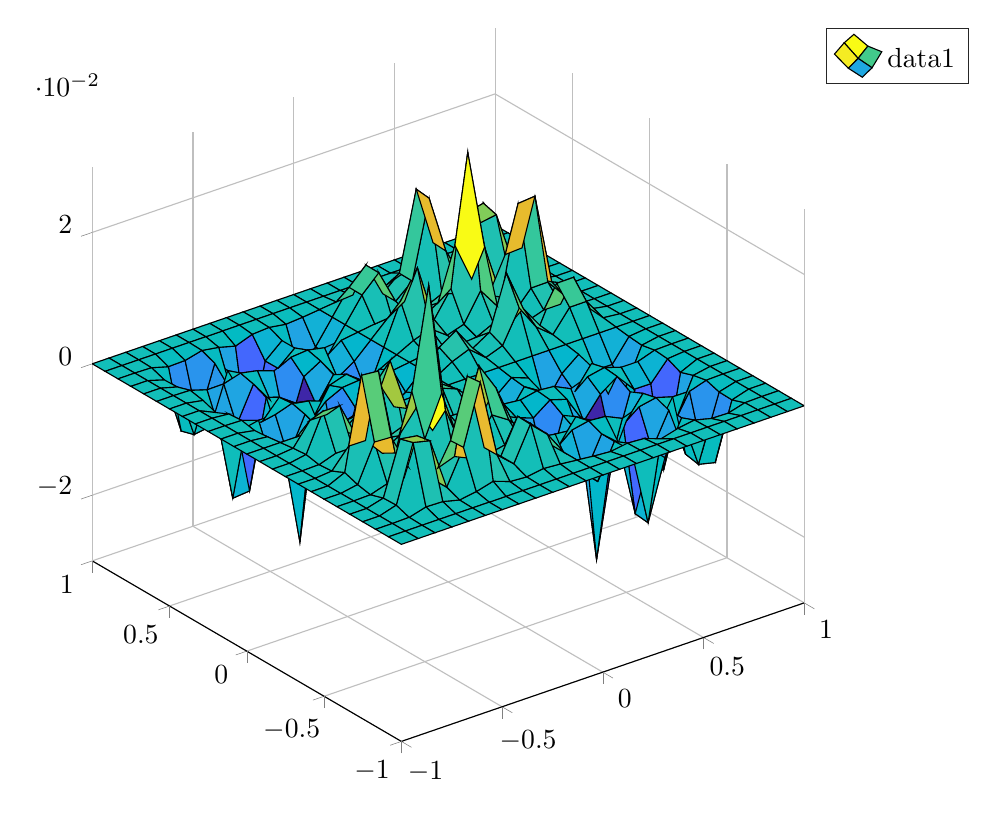
\begin{tikzpicture}

\begin{axis}[%
width=3.56in,
height=3.566in,
at={(0.597in,0.481in)},
scale only axis,
xmin=-1,
xmax=1,
tick align=outside,
ymin=-1,
ymax=1,
zmin=-0.03,
zmax=0.03,
view={-37.5}{30},
axis background/.style={fill=white},
axis x line*=bottom,
axis y line*=left,
axis z line*=left,
xmajorgrids,
ymajorgrids,
zmajorgrids,
legend style={at={(1.03,1)}, anchor=north west, legend cell align=left, align=left, draw=white!15!black}
]

\addplot3[%
surf,
shader=flat corner, draw=black, z buffer=sort, colormap={mymap}{[1pt] rgb(0pt)=(0.2422,0.1504,0.6603); rgb(1pt)=(0.25039,0.164995,0.707614); rgb(2pt)=(0.257771,0.181781,0.751138); rgb(3pt)=(0.264729,0.197757,0.795214); rgb(4pt)=(0.270648,0.214676,0.836371); rgb(5pt)=(0.275114,0.234238,0.870986); rgb(6pt)=(0.2783,0.255871,0.899071); rgb(7pt)=(0.280333,0.278233,0.9221); rgb(8pt)=(0.281338,0.300595,0.941376); rgb(9pt)=(0.281014,0.322757,0.957886); rgb(10pt)=(0.279467,0.344671,0.971676); rgb(11pt)=(0.275971,0.366681,0.982905); rgb(12pt)=(0.269914,0.3892,0.9906); rgb(13pt)=(0.260243,0.412329,0.995157); rgb(14pt)=(0.244033,0.435833,0.998833); rgb(15pt)=(0.220643,0.460257,0.997286); rgb(16pt)=(0.196333,0.484719,0.989152); rgb(17pt)=(0.183405,0.507371,0.979795); rgb(18pt)=(0.178643,0.528857,0.968157); rgb(19pt)=(0.176438,0.549905,0.952019); rgb(20pt)=(0.168743,0.570262,0.935871); rgb(21pt)=(0.154,0.5902,0.9218); rgb(22pt)=(0.146029,0.609119,0.907857); rgb(23pt)=(0.138024,0.627629,0.89729); rgb(24pt)=(0.124814,0.645929,0.888343); rgb(25pt)=(0.111252,0.6635,0.876314); rgb(26pt)=(0.0952095,0.679829,0.859781); rgb(27pt)=(0.0688714,0.694771,0.839357); rgb(28pt)=(0.0296667,0.708167,0.816333); rgb(29pt)=(0.00357143,0.720267,0.7917); rgb(30pt)=(0.00665714,0.731214,0.766014); rgb(31pt)=(0.0433286,0.741095,0.73941); rgb(32pt)=(0.0963952,0.75,0.712038); rgb(33pt)=(0.140771,0.7584,0.684157); rgb(34pt)=(0.1717,0.766962,0.655443); rgb(35pt)=(0.193767,0.775767,0.6251); rgb(36pt)=(0.216086,0.7843,0.5923); rgb(37pt)=(0.246957,0.791795,0.556743); rgb(38pt)=(0.290614,0.79729,0.518829); rgb(39pt)=(0.340643,0.8008,0.478857); rgb(40pt)=(0.3909,0.802871,0.435448); rgb(41pt)=(0.445629,0.802419,0.390919); rgb(42pt)=(0.5044,0.7993,0.348); rgb(43pt)=(0.561562,0.794233,0.304481); rgb(44pt)=(0.617395,0.787619,0.261238); rgb(45pt)=(0.671986,0.779271,0.2227); rgb(46pt)=(0.7242,0.769843,0.191029); rgb(47pt)=(0.773833,0.759805,0.16461); rgb(48pt)=(0.820314,0.749814,0.153529); rgb(49pt)=(0.863433,0.7406,0.159633); rgb(50pt)=(0.903543,0.733029,0.177414); rgb(51pt)=(0.939257,0.728786,0.209957); rgb(52pt)=(0.972757,0.729771,0.239443); rgb(53pt)=(0.995648,0.743371,0.237148); rgb(54pt)=(0.996986,0.765857,0.219943); rgb(55pt)=(0.995205,0.789252,0.202762); rgb(56pt)=(0.9892,0.813567,0.188533); rgb(57pt)=(0.978629,0.838629,0.176557); rgb(58pt)=(0.967648,0.8639,0.16429); rgb(59pt)=(0.96101,0.889019,0.153676); rgb(60pt)=(0.959671,0.913457,0.142257); rgb(61pt)=(0.962795,0.937338,0.12651); rgb(62pt)=(0.969114,0.960629,0.106362); rgb(63pt)=(0.9769,0.9839,0.0805)}, mesh/rows=25]
table[row sep=crcr, point meta=\thisrow{c}] {%
%
x	y	z	c\\
-1	-1	0	0\\
-0.916666666666667	-1	0	0\\
-0.833333333333333	-1	1.02695723625141e-24	1.02695723625141e-24\\
-0.75	-1	0	0\\
-0.666666666666667	-1	0	0\\
-0.583333333333333	-1	0	0\\
-0.5	-1	0	0\\
-0.416666666666667	-1	0	0\\
-0.333333333333333	-1	0	0\\
-0.25	-1	0	0\\
-0.166666666666667	-1	0	0\\
-0.0833333333333334	-1	0	0\\
0	-1	0	0\\
0.0833333333333333	-1	0	0\\
0.166666666666667	-1	0	0\\
0.25	-1	0	0\\
0.333333333333333	-1	0	0\\
0.416666666666667	-1	0	0\\
0.5	-1	0	0\\
0.583333333333333	-1	0	0\\
0.666666666666667	-1	0	0\\
0.75	-1	0	0\\
0.833333333333333	-1	0	0\\
0.916666666666667	-1	-4.38399307163469e-27	-4.38399307163469e-27\\
1	-1	0	0\\
-1	-0.916666666666667	0	0\\
-0.916666666666667	-0.916666666666667	2.55753406345044e-09	2.55753406345044e-09\\
-0.833333333333333	-0.916666666666667	3.85777718973534e-07	3.85777718973534e-07\\
-0.75	-0.916666666666667	4.17100875631788e-06	4.17100875631788e-06\\
-0.666666666666667	-0.916666666666667	3.64929550800072e-06	3.64929550800072e-06\\
-0.583333333333333	-0.916666666666667	3.45860111752149e-07	3.45860111752149e-07\\
-0.5	-0.916666666666667	2.33954300020683e-06	2.33954300020683e-06\\
-0.416666666666667	-0.916666666666667	5.70854139583692e-06	5.70854139583692e-06\\
-0.333333333333333	-0.916666666666667	1.17920908563584e-06	1.17920908563584e-06\\
-0.25	-0.916666666666667	3.45029265806706e-07	3.45029265806706e-07\\
-0.166666666666667	-0.916666666666667	2.26755661545572e-06	2.26755661545572e-06\\
-0.0833333333333334	-0.916666666666667	1.33785564740444e-06	1.33785564740444e-06\\
0	-0.916666666666667	-4.2425755489483e-22	-4.2425755489483e-22\\
0.0833333333333333	-0.916666666666667	-1.33785564740444e-06	-1.33785564740444e-06\\
0.166666666666667	-0.916666666666667	-2.26755661545571e-06	-2.26755661545571e-06\\
0.25	-0.916666666666667	-3.45029265806705e-07	-3.45029265806705e-07\\
0.333333333333333	-0.916666666666667	-1.17920908563584e-06	-1.17920908563584e-06\\
0.416666666666667	-0.916666666666667	-5.70854139583693e-06	-5.70854139583693e-06\\
0.5	-0.916666666666667	-2.33954300020683e-06	-2.33954300020683e-06\\
0.583333333333333	-0.916666666666667	-3.4586011175215e-07	-3.4586011175215e-07\\
0.666666666666667	-0.916666666666667	-3.64929550800072e-06	-3.64929550800072e-06\\
0.75	-0.916666666666667	-4.17100875631788e-06	-4.17100875631788e-06\\
0.833333333333333	-0.916666666666667	-3.85777718973533e-07	-3.85777718973533e-07\\
0.916666666666667	-0.916666666666667	-2.55753406345042e-09	-2.55753406345042e-09\\
1	-0.916666666666667	0	0\\
-1	-0.833333333333333	1.02695723625141e-24	1.02695723625141e-24\\
-0.916666666666667	-0.833333333333333	3.85777718973533e-07	3.85777718973533e-07\\
-0.833333333333333	-0.833333333333333	6.71198962422951e-05	6.71198962422951e-05\\
-0.75	-0.833333333333333	0.000778127800887982	0.000778127800887982\\
-0.666666666666667	-0.833333333333333	0.000707315736756557	0.000707315736756557\\
-0.583333333333333	-0.833333333333333	6.86074746915453e-05	6.86074746915453e-05\\
-0.5	-0.833333333333333	0.000471138162446881	0.000471138162446881\\
-0.416666666666667	-0.833333333333333	0.00116140316014542	0.00116140316014542\\
-0.333333333333333	-0.833333333333333	0.000241610914204461	0.000241610914204461\\
-0.25	-0.833333333333333	7.10368896279139e-05	7.10368896279139e-05\\
-0.166666666666667	-0.833333333333333	0.000468336406285743	0.000468336406285743\\
-0.0833333333333334	-0.833333333333333	0.000276812375771035	0.000276812375771035\\
0	-0.833333333333333	-7.74552301490904e-20	-7.74552301490904e-20\\
0.0833333333333333	-0.833333333333333	-0.000276812375771035	-0.000276812375771035\\
0.166666666666667	-0.833333333333333	-0.000468336406285742	-0.000468336406285742\\
0.25	-0.833333333333333	-7.10368896279136e-05	-7.10368896279136e-05\\
0.333333333333333	-0.833333333333333	-0.00024161091420446	-0.00024161091420446\\
0.416666666666667	-0.833333333333333	-0.00116140316014542	-0.00116140316014542\\
0.5	-0.833333333333333	-0.000471138162446881	-0.000471138162446881\\
0.583333333333333	-0.833333333333333	-6.86074746915456e-05	-6.86074746915456e-05\\
0.666666666666667	-0.833333333333333	-0.000707315736756559	-0.000707315736756559\\
0.75	-0.833333333333333	-0.000778127800887981	-0.000778127800887981\\
0.833333333333333	-0.833333333333333	-6.7119896242295e-05	-6.7119896242295e-05\\
0.916666666666667	-0.833333333333333	-3.85777718973525e-07	-3.85777718973525e-07\\
1	-0.833333333333333	-1.0269572362514e-24	-1.0269572362514e-24\\
-1	-0.75	0	0\\
-0.916666666666667	-0.75	4.17100875631788e-06	4.17100875631788e-06\\
-0.833333333333333	-0.75	0.000778127800887983	0.000778127800887983\\
-0.75	-0.75	0.00943571698715445	0.00943571698715445\\
-0.666666666666667	-0.75	0.00882480124123988	0.00882480124123988\\
-0.583333333333333	-0.75	0.000872104526134152	0.000872104526134152\\
-0.5	-0.75	0.0060652983794619	0.0060652983794619\\
-0.416666666666667	-0.75	0.0150841772008774	0.0150841772008774\\
-0.333333333333333	-0.75	0.00315753528677166	0.00315753528677166\\
-0.25	-0.75	0.000932352964394895	0.000932352964394895\\
-0.166666666666667	-0.75	0.00616423466770155	0.00616423466770155\\
-0.0833333333333334	-0.75	0.00364924259814257	0.00364924259814257\\
0	-0.75	-8.76737641779841e-19	-8.76737641779841e-19\\
0.0833333333333333	-0.75	-0.00364924259814257	-0.00364924259814257\\
0.166666666666667	-0.75	-0.00616423466770154	-0.00616423466770154\\
0.25	-0.75	-0.000932352964394891	-0.000932352964394891\\
0.333333333333333	-0.75	-0.00315753528677164	-0.00315753528677164\\
0.416666666666667	-0.75	-0.0150841772008774	-0.0150841772008774\\
0.5	-0.75	-0.0060652983794619	-0.0060652983794619\\
0.583333333333333	-0.75	-0.000872104526134156	-0.000872104526134156\\
0.666666666666667	-0.75	-0.00882480124123989	-0.00882480124123989\\
0.75	-0.75	-0.00943571698715444	-0.00943571698715444\\
0.833333333333333	-0.75	-0.000778127800887982	-0.000778127800887982\\
0.916666666666667	-0.75	-4.17100875631781e-06	-4.17100875631781e-06\\
1	-0.75	0	0\\
-1	-0.666666666666667	0	0\\
-0.916666666666667	-0.666666666666667	3.64929550800072e-06	3.64929550800072e-06\\
-0.833333333333333	-0.666666666666667	0.000707315736756557	0.000707315736756557\\
-0.75	-0.666666666666667	0.00882480124123988	0.00882480124123988\\
-0.666666666666667	-0.666666666666667	0.00842066215543398	0.00842066215543398\\
-0.583333333333333	-0.666666666666667	0.000843966898384536	0.000843966898384536\\
-0.5	-0.666666666666667	0.00592857826938018	0.00592857826938018\\
-0.416666666666667	-0.666666666666667	0.0148502404760497	0.0148502404760497\\
-0.333333333333333	-0.666666666666667	0.00312456184123599	0.00312456184123599\\
-0.25	-0.666666666666667	0.000925942478032866	0.000925942478032866\\
-0.166666666666667	-0.666666666666667	0.00613646636398126	0.00613646636398126\\
-0.0833333333333334	-0.666666666666667	0.00363775449063844	0.00363775449063844\\
0	-0.666666666666667	-8.44331861748012e-19	-8.44331861748012e-19\\
0.0833333333333333	-0.666666666666667	-0.00363775449063844	-0.00363775449063844\\
0.166666666666667	-0.666666666666667	-0.00613646636398124	-0.00613646636398124\\
0.25	-0.666666666666667	-0.000925942478032862	-0.000925942478032862\\
0.333333333333333	-0.666666666666667	-0.00312456184123597	-0.00312456184123597\\
0.416666666666667	-0.666666666666667	-0.0148502404760497	-0.0148502404760497\\
0.5	-0.666666666666667	-0.00592857826938018	-0.00592857826938018\\
0.583333333333333	-0.666666666666667	-0.00084396689838454	-0.00084396689838454\\
0.666666666666667	-0.666666666666667	-0.00842066215543399	-0.00842066215543399\\
0.75	-0.666666666666667	-0.00882480124123987	-0.00882480124123987\\
0.833333333333333	-0.666666666666667	-0.000707315736756558	-0.000707315736756558\\
0.916666666666667	-0.666666666666667	-3.64929550800066e-06	-3.64929550800066e-06\\
1	-0.666666666666667	0	0\\
-1	-0.583333333333333	0	0\\
-0.916666666666667	-0.583333333333333	3.45860111752149e-07	3.45860111752149e-07\\
-0.833333333333333	-0.583333333333333	6.86074746915453e-05	6.86074746915453e-05\\
-0.75	-0.583333333333333	0.000872104526134152	0.000872104526134152\\
-0.666666666666667	-0.583333333333333	0.000843966898384536	0.000843966898384536\\
-0.583333333333333	-0.583333333333333	8.50681297213606e-05	8.50681297213606e-05\\
-0.5	-0.583333333333333	0.000592761470027727	0.000592761470027727\\
-0.416666666666667	-0.583333333333333	0.00149315597727987	0.00149315597727987\\
-0.333333333333333	-0.583333333333333	0.000315453871556334	0.000315453871556334\\
-0.25	-0.583333333333333	9.31814902686496e-05	9.31814902686496e-05\\
-0.166666666666667	-0.583333333333333	0.000618502248354859	0.000618502248354859\\
-0.0833333333333334	-0.583333333333333	0.000367064223668659	0.000367064223668659\\
0	-0.583333333333333	-7.40930762219607e-20	-7.40930762219607e-20\\
0.0833333333333333	-0.583333333333333	-0.000367064223668659	-0.000367064223668659\\
0.166666666666667	-0.583333333333333	-0.000618502248354857	-0.000618502248354857\\
0.25	-0.583333333333333	-9.31814902686491e-05	-9.31814902686491e-05\\
0.333333333333333	-0.583333333333333	-0.000315453871556332	-0.000315453871556332\\
0.416666666666667	-0.583333333333333	-0.00149315597727987	-0.00149315597727987\\
0.5	-0.583333333333333	-0.000592761470027727	-0.000592761470027727\\
0.583333333333333	-0.583333333333333	-8.50681297213611e-05	-8.50681297213611e-05\\
0.666666666666667	-0.583333333333333	-0.000843966898384538	-0.000843966898384538\\
0.75	-0.583333333333333	-0.00087210452613415	-0.00087210452613415\\
0.833333333333333	-0.583333333333333	-6.86074746915454e-05	-6.86074746915454e-05\\
0.916666666666667	-0.583333333333333	-3.45860111752143e-07	-3.45860111752143e-07\\
1	-0.583333333333333	0	0\\
-1	-0.5	0	0\\
-0.916666666666667	-0.5	2.33954300020683e-06	2.33954300020683e-06\\
-0.833333333333333	-0.5	0.000471138162446881	0.000471138162446881\\
-0.75	-0.5	0.0060652983794619	0.0060652983794619\\
-0.666666666666667	-0.5	0.00592857826938018	0.00592857826938018\\
-0.583333333333333	-0.5	0.000592761470027727	0.000592761470027727\\
-0.5	-0.5	0.00393294666281547	0.00393294666281547\\
-0.416666666666667	-0.5	0.00994977833558941	0.00994977833558941\\
-0.333333333333333	-0.5	0.00210867680461956	0.00210867680461956\\
-0.25	-0.5	0.000610455051438689	0.000610455051438689\\
-0.166666666666667	-0.5	0.00405241439845992	0.00405241439845992\\
-0.0833333333333334	-0.5	0.0024071556172955	0.0024071556172955\\
0	-0.5	-5.91805759022251e-19	-5.91805759022251e-19\\
0.0833333333333333	-0.5	-0.0024071556172955	-0.0024071556172955\\
0.166666666666667	-0.5	-0.00405241439845991	-0.00405241439845991\\
0.25	-0.5	-0.000610455051438686	-0.000610455051438686\\
0.333333333333333	-0.5	-0.00210867680461956	-0.00210867680461956\\
0.416666666666667	-0.5	-0.00994977833558942	-0.00994977833558942\\
0.5	-0.5	-0.00393294666281547	-0.00393294666281547\\
0.583333333333333	-0.5	-0.000592761470027729	-0.000592761470027729\\
0.666666666666667	-0.5	-0.00592857826938019	-0.00592857826938019\\
0.75	-0.5	-0.00606529837946189	-0.00606529837946189\\
0.833333333333333	-0.5	-0.000471138162446881	-0.000471138162446881\\
0.916666666666667	-0.5	-2.33954300020679e-06	-2.33954300020679e-06\\
1	-0.5	0	0\\
-1	-0.416666666666667	0	0\\
-0.916666666666667	-0.416666666666667	5.70854139583692e-06	5.70854139583692e-06\\
-0.833333333333333	-0.416666666666667	0.00116140316014542	0.00116140316014542\\
-0.75	-0.416666666666667	0.0150841772008774	0.0150841772008774\\
-0.666666666666667	-0.416666666666667	0.0148502404760497	0.0148502404760497\\
-0.583333333333333	-0.416666666666667	0.00149315597727987	0.00149315597727987\\
-0.5	-0.416666666666667	0.00994977833558941	0.00994977833558941\\
-0.416666666666667	-0.416666666666667	0.0252552578198303	0.0252552578198303\\
-0.333333333333333	-0.416666666666667	0.00536572588063085	0.00536572588063085\\
-0.25	-0.416666666666667	0.00155612453270233	0.00155612453270233\\
-0.166666666666667	-0.416666666666667	0.010342674976464	0.010342674976464\\
-0.0833333333333334	-0.416666666666667	0.00614793627719881	0.00614793627719881\\
0	-0.416666666666667	-1.50433859765667e-18	-1.50433859765667e-18\\
0.0833333333333333	-0.416666666666667	-0.0061479362771988	-0.0061479362771988\\
0.166666666666667	-0.416666666666667	-0.010342674976464	-0.010342674976464\\
0.25	-0.416666666666667	-0.00155612453270232	-0.00155612453270232\\
0.333333333333333	-0.416666666666667	-0.00536572588063083	-0.00536572588063083\\
0.416666666666667	-0.416666666666667	-0.0252552578198304	-0.0252552578198304\\
0.5	-0.416666666666667	-0.00994977833558941	-0.00994977833558941\\
0.583333333333333	-0.416666666666667	-0.00149315597727988	-0.00149315597727988\\
0.666666666666667	-0.416666666666667	-0.0148502404760497	-0.0148502404760497\\
0.75	-0.416666666666667	-0.0150841772008774	-0.0150841772008774\\
0.833333333333333	-0.416666666666667	-0.00116140316014542	-0.00116140316014542\\
0.916666666666667	-0.416666666666667	-5.70854139583682e-06	-5.70854139583682e-06\\
1	-0.416666666666667	0	0\\
-1	-0.333333333333333	0	0\\
-0.916666666666667	-0.333333333333333	1.17920908563584e-06	1.17920908563584e-06\\
-0.833333333333333	-0.333333333333333	0.000241610914204461	0.000241610914204461\\
-0.75	-0.333333333333333	0.00315753528677166	0.00315753528677166\\
-0.666666666666667	-0.333333333333333	0.00312456184123599	0.00312456184123599\\
-0.583333333333333	-0.333333333333333	0.000315453871556334	0.000315453871556334\\
-0.5	-0.333333333333333	0.00210867680461956	0.00210867680461956\\
-0.416666666666667	-0.333333333333333	0.00536572588063085	0.00536572588063085\\
-0.333333333333333	-0.333333333333333	0.00114214387023767	0.00114214387023767\\
-0.25	-0.333333333333333	0.000331677317790113	0.000331677317790113\\
-0.166666666666667	-0.333333333333333	0.00220651736235955	0.00220651736235955\\
-0.0833333333333334	-0.333333333333333	0.00131231582712499	0.00131231582712499\\
0	-0.333333333333333	-3.16585135024486e-19	-3.16585135024486e-19\\
0.0833333333333333	-0.333333333333333	-0.00131231582712499	-0.00131231582712499\\
0.166666666666667	-0.333333333333333	-0.00220651736235954	-0.00220651736235954\\
0.25	-0.333333333333333	-0.000331677317790112	-0.000331677317790112\\
0.333333333333333	-0.333333333333333	-0.00114214387023766	-0.00114214387023766\\
0.416666666666667	-0.333333333333333	-0.00536572588063086	-0.00536572588063086\\
0.5	-0.333333333333333	-0.00210867680461956	-0.00210867680461956\\
0.583333333333333	-0.333333333333333	-0.000315453871556335	-0.000315453871556335\\
0.666666666666667	-0.333333333333333	-0.00312456184123599	-0.00312456184123599\\
0.75	-0.333333333333333	-0.00315753528677165	-0.00315753528677165\\
0.833333333333333	-0.333333333333333	-0.000241610914204461	-0.000241610914204461\\
0.916666666666667	-0.333333333333333	-1.17920908563582e-06	-1.17920908563582e-06\\
1	-0.333333333333333	0	0\\
-1	-0.25	0	0\\
-0.916666666666667	-0.25	3.45029265806706e-07	3.45029265806706e-07\\
-0.833333333333333	-0.25	7.1036889627914e-05	7.1036889627914e-05\\
-0.75	-0.25	0.000932352964394894	0.000932352964394894\\
-0.666666666666667	-0.25	0.000925942478032866	0.000925942478032866\\
-0.583333333333333	-0.25	9.31814902686495e-05	9.31814902686495e-05\\
-0.5	-0.25	0.000610455051438689	0.000610455051438689\\
-0.416666666666667	-0.25	0.00155612453270233	0.00155612453270233\\
-0.333333333333333	-0.25	0.000331677317790113	0.000331677317790113\\
-0.25	-0.25	9.54350634367825e-05	9.54350634367825e-05\\
-0.166666666666667	-0.25	0.000634901021554919	0.000634901021554919\\
-0.0833333333333334	-0.25	0.00037775454883306	0.00037775454883306\\
0	-0.25	-8.80499813311504e-20	-8.80499813311504e-20\\
0.0833333333333333	-0.25	-0.00037775454883306	-0.00037775454883306\\
0.166666666666667	-0.25	-0.000634901021554917	-0.000634901021554917\\
0.25	-0.25	-9.54350634367821e-05	-9.54350634367821e-05\\
0.333333333333333	-0.25	-0.000331677317790112	-0.000331677317790112\\
0.416666666666667	-0.25	-0.00155612453270233	-0.00155612453270233\\
0.5	-0.25	-0.000610455051438689	-0.000610455051438689\\
0.583333333333333	-0.25	-9.31814902686498e-05	-9.31814902686498e-05\\
0.666666666666667	-0.25	-0.000925942478032867	-0.000925942478032867\\
0.75	-0.25	-0.000932352964394893	-0.000932352964394893\\
0.833333333333333	-0.25	-7.1036889627914e-05	-7.1036889627914e-05\\
0.916666666666667	-0.25	-3.450292658067e-07	-3.450292658067e-07\\
1	-0.25	0	0\\
-1	-0.166666666666667	0	0\\
-0.916666666666667	-0.166666666666667	2.26755661545572e-06	2.26755661545572e-06\\
-0.833333333333333	-0.166666666666667	0.000468336406285743	0.000468336406285743\\
-0.75	-0.166666666666667	0.00616423466770155	0.00616423466770155\\
-0.666666666666667	-0.166666666666667	0.00613646636398126	0.00613646636398126\\
-0.583333333333333	-0.166666666666667	0.000618502248354858	0.000618502248354858\\
-0.5	-0.166666666666667	0.00405241439845992	0.00405241439845992\\
-0.416666666666667	-0.166666666666667	0.010342674976464	0.010342674976464\\
-0.333333333333333	-0.166666666666667	0.00220651736235955	0.00220651736235955\\
-0.25	-0.166666666666667	0.000634901021554919	0.000634901021554919\\
-0.166666666666667	-0.166666666666667	0.00422559650685534	0.00422559650685534\\
-0.0833333333333334	-0.166666666666667	0.00251483803933617	0.00251483803933617\\
0	-0.166666666666667	-6.34758211468699e-19	-6.34758211468699e-19\\
0.0833333333333333	-0.166666666666667	-0.00251483803933617	-0.00251483803933617\\
0.166666666666667	-0.166666666666667	-0.00422559650685533	-0.00422559650685533\\
0.25	-0.166666666666667	-0.000634901021554916	-0.000634901021554916\\
0.333333333333333	-0.166666666666667	-0.00220651736235954	-0.00220651736235954\\
0.416666666666667	-0.166666666666667	-0.010342674976464	-0.010342674976464\\
0.5	-0.166666666666667	-0.00405241439845992	-0.00405241439845992\\
0.583333333333333	-0.166666666666667	-0.000618502248354861	-0.000618502248354861\\
0.666666666666667	-0.166666666666667	-0.00613646636398127	-0.00613646636398127\\
0.75	-0.166666666666667	-0.00616423466770154	-0.00616423466770154\\
0.833333333333333	-0.166666666666667	-0.000468336406285743	-0.000468336406285743\\
0.916666666666667	-0.166666666666667	-2.26755661545568e-06	-2.26755661545568e-06\\
1	-0.166666666666667	0	0\\
-1	-0.0833333333333334	0	0\\
-0.916666666666667	-0.0833333333333334	1.33785564740444e-06	1.33785564740444e-06\\
-0.833333333333333	-0.0833333333333334	0.000276812375771035	0.000276812375771035\\
-0.75	-0.0833333333333334	0.00364924259814257	0.00364924259814257\\
-0.666666666666667	-0.0833333333333334	0.00363775449063844	0.00363775449063844\\
-0.583333333333333	-0.0833333333333334	0.000367064223668659	0.000367064223668659\\
-0.5	-0.0833333333333334	0.0024071556172955	0.0024071556172955\\
-0.416666666666667	-0.0833333333333334	0.0061479362771988	0.0061479362771988\\
-0.333333333333333	-0.0833333333333334	0.00131231582712499	0.00131231582712499\\
-0.25	-0.0833333333333334	0.00037775454883306	0.00037775454883306\\
-0.166666666666667	-0.0833333333333334	0.00251483803933617	0.00251483803933617\\
-0.0833333333333334	-0.0833333333333334	0.0014969284339611	0.0014969284339611\\
0	-0.0833333333333334	-4.12134423225633e-19	-4.12134423225633e-19\\
0.0833333333333333	-0.0833333333333334	-0.0014969284339611	-0.0014969284339611\\
0.166666666666667	-0.0833333333333334	-0.00251483803933616	-0.00251483803933616\\
0.25	-0.0833333333333334	-0.000377754548833058	-0.000377754548833058\\
0.333333333333333	-0.0833333333333334	-0.00131231582712498	-0.00131231582712498\\
0.416666666666667	-0.0833333333333334	-0.00614793627719881	-0.00614793627719881\\
0.5	-0.0833333333333334	-0.00240715561729551	-0.00240715561729551\\
0.583333333333333	-0.0833333333333334	-0.000367064223668661	-0.000367064223668661\\
0.666666666666667	-0.0833333333333334	-0.00363775449063844	-0.00363775449063844\\
0.75	-0.0833333333333334	-0.00364924259814256	-0.00364924259814256\\
0.833333333333333	-0.0833333333333334	-0.000276812375771035	-0.000276812375771035\\
0.916666666666667	-0.0833333333333334	-1.33785564740442e-06	-1.33785564740442e-06\\
1	-0.0833333333333334	0	0\\
-1	0	0	0\\
-0.916666666666667	0	-4.22019650749432e-22	-4.22019650749432e-22\\
-0.833333333333333	0	-7.58062703141482e-20	-7.58062703141482e-20\\
-0.75	0	-8.8948973557021e-19	-8.8948973557021e-19\\
-0.666666666666667	0	-8.48925864908015e-19	-8.48925864908015e-19\\
-0.583333333333333	0	-7.4663668535476e-20	-7.4663668535476e-20\\
-0.5	0	-6.59299545930563e-19	-6.59299545930563e-19\\
-0.416666666666667	0	-1.65655633099897e-18	-1.65655633099897e-18\\
-0.333333333333333	0	-3.57084812293917e-19	-3.57084812293917e-19\\
-0.25	0	-8.37743870326049e-20	-8.37743870326049e-20\\
-0.166666666666667	0	-6.03879200828298e-19	-6.03879200828298e-19\\
-0.0833333333333334	0	-3.932851103973e-19	-3.932851103973e-19\\
0	0	-4.82118586296267e-21	-4.82118586296267e-21\\
0.0833333333333333	0	4.48056541275829e-19	4.48056541275829e-19\\
0.166666666666667	0	6.75165917404855e-19	6.75165917404855e-19\\
0.25	0	8.05379513898792e-20	8.05379513898792e-20\\
0.333333333333333	0	3.00487456194101e-19	3.00487456194101e-19\\
0.416666666666667	0	1.62580333661468e-18	1.62580333661468e-18\\
0.5	0	5.57212921187685e-19	5.57212921187685e-19\\
0.583333333333333	0	9.80093456331336e-20	9.80093456331336e-20\\
0.666666666666667	0	8.61737011716055e-19	8.61737011716055e-19\\
0.75	0	9.60761298722394e-19	9.60761298722394e-19\\
0.833333333333333	0	7.99192795843061e-20	7.99192795843061e-20\\
0.916666666666667	0	3.15236993062634e-22	3.15236993062634e-22\\
1	0	0	0\\
-1	0.0833333333333333	0	0\\
-0.916666666666667	0.0833333333333333	-1.33785564740444e-06	-1.33785564740444e-06\\
-0.833333333333333	0.0833333333333333	-0.000276812375771035	-0.000276812375771035\\
-0.75	0.0833333333333333	-0.00364924259814257	-0.00364924259814257\\
-0.666666666666667	0.0833333333333333	-0.00363775449063844	-0.00363775449063844\\
-0.583333333333333	0.0833333333333333	-0.000367064223668659	-0.000367064223668659\\
-0.5	0.0833333333333333	-0.0024071556172955	-0.0024071556172955\\
-0.416666666666667	0.0833333333333333	-0.0061479362771988	-0.0061479362771988\\
-0.333333333333333	0.0833333333333333	-0.00131231582712499	-0.00131231582712499\\
-0.25	0.0833333333333333	-0.00037775454883306	-0.00037775454883306\\
-0.166666666666667	0.0833333333333333	-0.00251483803933617	-0.00251483803933617\\
-0.0833333333333334	0.0833333333333333	-0.0014969284339611	-0.0014969284339611\\
0	0.0833333333333333	4.51410925247731e-19	4.51410925247731e-19\\
0.0833333333333333	0.0833333333333333	0.0014969284339611	0.0014969284339611\\
0.166666666666667	0.0833333333333333	0.00251483803933616	0.00251483803933616\\
0.25	0.0833333333333333	0.000377754548833058	0.000377754548833058\\
0.333333333333333	0.0833333333333333	0.00131231582712498	0.00131231582712498\\
0.416666666666667	0.0833333333333333	0.00614793627719881	0.00614793627719881\\
0.5	0.0833333333333333	0.0024071556172955	0.0024071556172955\\
0.583333333333333	0.0833333333333333	0.00036706422366866	0.00036706422366866\\
0.666666666666667	0.0833333333333333	0.00363775449063844	0.00363775449063844\\
0.75	0.0833333333333333	0.00364924259814256	0.00364924259814256\\
0.833333333333333	0.0833333333333333	0.000276812375771035	0.000276812375771035\\
0.916666666666667	0.0833333333333333	1.33785564740442e-06	1.33785564740442e-06\\
1	0.0833333333333333	0	0\\
-1	0.166666666666667	0	0\\
-0.916666666666667	0.166666666666667	-2.26755661545571e-06	-2.26755661545571e-06\\
-0.833333333333333	0.166666666666667	-0.000468336406285741	-0.000468336406285741\\
-0.75	0.166666666666667	-0.00616423466770153	-0.00616423466770153\\
-0.666666666666667	0.166666666666667	-0.00613646636398124	-0.00613646636398124\\
-0.583333333333333	0.166666666666667	-0.000618502248354857	-0.000618502248354857\\
-0.5	0.166666666666667	-0.00405241439845991	-0.00405241439845991\\
-0.416666666666667	0.166666666666667	-0.010342674976464	-0.010342674976464\\
-0.333333333333333	0.166666666666667	-0.00220651736235954	-0.00220651736235954\\
-0.25	0.166666666666667	-0.000634901021554917	-0.000634901021554917\\
-0.166666666666667	0.166666666666667	-0.00422559650685533	-0.00422559650685533\\
-0.0833333333333334	0.166666666666667	-0.00251483803933616	-0.00251483803933616\\
0	0.166666666666667	6.9848421185914e-19	6.9848421185914e-19\\
0.0833333333333333	0.166666666666667	0.00251483803933616	0.00251483803933616\\
0.166666666666667	0.166666666666667	0.00422559650685532	0.00422559650685532\\
0.25	0.166666666666667	0.000634901021554914	0.000634901021554914\\
0.333333333333333	0.166666666666667	0.00220651736235953	0.00220651736235953\\
0.416666666666667	0.166666666666667	0.010342674976464	0.010342674976464\\
0.5	0.166666666666667	0.00405241439845991	0.00405241439845991\\
0.583333333333333	0.166666666666667	0.000618502248354859	0.000618502248354859\\
0.666666666666667	0.166666666666667	0.00613646636398125	0.00613646636398125\\
0.75	0.166666666666667	0.00616423466770152	0.00616423466770152\\
0.833333333333333	0.166666666666667	0.000468336406285741	0.000468336406285741\\
0.916666666666667	0.166666666666667	2.26755661545567e-06	2.26755661545567e-06\\
1	0.166666666666667	0	0\\
-1	0.25	0	0\\
-0.916666666666667	0.25	-3.45029265806704e-07	-3.45029265806704e-07\\
-0.833333333333333	0.25	-7.10368896279136e-05	-7.10368896279136e-05\\
-0.75	0.25	-0.000932352964394891	-0.000932352964394891\\
-0.666666666666667	0.25	-0.000925942478032862	-0.000925942478032862\\
-0.583333333333333	0.25	-9.31814902686491e-05	-9.31814902686491e-05\\
-0.5	0.25	-0.000610455051438686	-0.000610455051438686\\
-0.416666666666667	0.25	-0.00155612453270232	-0.00155612453270232\\
-0.333333333333333	0.25	-0.000331677317790112	-0.000331677317790112\\
-0.25	0.25	-9.5435063436782e-05	-9.5435063436782e-05\\
-0.166666666666667	0.25	-0.000634901021554916	-0.000634901021554916\\
-0.0833333333333334	0.25	-0.000377754548833058	-0.000377754548833058\\
0	0.25	7.94089675468141e-20	7.94089675468141e-20\\
0.0833333333333333	0.25	0.000377754548833058	0.000377754548833058\\
0.166666666666667	0.25	0.000634901021554914	0.000634901021554914\\
0.25	0.25	9.54350634367817e-05	9.54350634367817e-05\\
0.333333333333333	0.25	0.000331677317790111	0.000331677317790111\\
0.416666666666667	0.25	0.00155612453270232	0.00155612453270232\\
0.5	0.25	0.000610455051438686	0.000610455051438686\\
0.583333333333333	0.25	9.31814902686495e-05	9.31814902686495e-05\\
0.666666666666667	0.25	0.000925942478032864	0.000925942478032864\\
0.75	0.25	0.000932352964394889	0.000932352964394889\\
0.833333333333333	0.25	7.10368896279137e-05	7.10368896279137e-05\\
0.916666666666667	0.25	3.45029265806699e-07	3.45029265806699e-07\\
1	0.25	0	0\\
-1	0.333333333333333	0	0\\
-0.916666666666667	0.333333333333333	-1.17920908563583e-06	-1.17920908563583e-06\\
-0.833333333333333	0.333333333333333	-0.00024161091420446	-0.00024161091420446\\
-0.75	0.333333333333333	-0.00315753528677164	-0.00315753528677164\\
-0.666666666666667	0.333333333333333	-0.00312456184123597	-0.00312456184123597\\
-0.583333333333333	0.333333333333333	-0.000315453871556332	-0.000315453871556332\\
-0.5	0.333333333333333	-0.00210867680461956	-0.00210867680461956\\
-0.416666666666667	0.333333333333333	-0.00536572588063083	-0.00536572588063083\\
-0.333333333333333	0.333333333333333	-0.00114214387023766	-0.00114214387023766\\
-0.25	0.333333333333333	-0.000331677317790112	-0.000331677317790112\\
-0.166666666666667	0.333333333333333	-0.00220651736235954	-0.00220651736235954\\
-0.0833333333333334	0.333333333333333	-0.00131231582712498	-0.00131231582712498\\
0	0.333333333333333	3.22485562489602e-19	3.22485562489602e-19\\
0.0833333333333333	0.333333333333333	0.00131231582712498	0.00131231582712498\\
0.166666666666667	0.333333333333333	0.00220651736235953	0.00220651736235953\\
0.25	0.333333333333333	0.000331677317790111	0.000331677317790111\\
0.333333333333333	0.333333333333333	0.00114214387023766	0.00114214387023766\\
0.416666666666667	0.333333333333333	0.00536572588063084	0.00536572588063084\\
0.5	0.333333333333333	0.00210867680461956	0.00210867680461956\\
0.583333333333333	0.333333333333333	0.000315453871556334	0.000315453871556334\\
0.666666666666667	0.333333333333333	0.00312456184123598	0.00312456184123598\\
0.75	0.333333333333333	0.00315753528677164	0.00315753528677164\\
0.833333333333333	0.333333333333333	0.00024161091420446	0.00024161091420446\\
0.916666666666667	0.333333333333333	1.17920908563582e-06	1.17920908563582e-06\\
1	0.333333333333333	0	0\\
-1	0.416666666666667	0	0\\
-0.916666666666667	0.416666666666667	-5.70854139583693e-06	-5.70854139583693e-06\\
-0.833333333333333	0.416666666666667	-0.00116140316014542	-0.00116140316014542\\
-0.75	0.416666666666667	-0.0150841772008774	-0.0150841772008774\\
-0.666666666666667	0.416666666666667	-0.0148502404760497	-0.0148502404760497\\
-0.583333333333333	0.416666666666667	-0.00149315597727987	-0.00149315597727987\\
-0.5	0.416666666666667	-0.00994977833558942	-0.00994977833558942\\
-0.416666666666667	0.416666666666667	-0.0252552578198304	-0.0252552578198304\\
-0.333333333333333	0.416666666666667	-0.00536572588063086	-0.00536572588063086\\
-0.25	0.416666666666667	-0.00155612453270233	-0.00155612453270233\\
-0.166666666666667	0.416666666666667	-0.010342674976464	-0.010342674976464\\
-0.0833333333333334	0.416666666666667	-0.00614793627719881	-0.00614793627719881\\
0	0.416666666666667	1.70743447471519e-18	1.70743447471519e-18\\
0.0833333333333333	0.416666666666667	0.00614793627719881	0.00614793627719881\\
0.166666666666667	0.416666666666667	0.010342674976464	0.010342674976464\\
0.25	0.416666666666667	0.00155612453270232	0.00155612453270232\\
0.333333333333333	0.416666666666667	0.00536572588063084	0.00536572588063084\\
0.416666666666667	0.416666666666667	0.0252552578198304	0.0252552578198304\\
0.5	0.416666666666667	0.00994977833558942	0.00994977833558942\\
0.583333333333333	0.416666666666667	0.00149315597727988	0.00149315597727988\\
0.666666666666667	0.416666666666667	0.0148502404760497	0.0148502404760497\\
0.75	0.416666666666667	0.0150841772008774	0.0150841772008774\\
0.833333333333333	0.416666666666667	0.00116140316014542	0.00116140316014542\\
0.916666666666667	0.416666666666667	5.70854139583684e-06	5.70854139583684e-06\\
1	0.416666666666667	0	0\\
-1	0.5	0	0\\
-0.916666666666667	0.5	-2.33954300020683e-06	-2.33954300020683e-06\\
-0.833333333333333	0.5	-0.000471138162446881	-0.000471138162446881\\
-0.75	0.5	-0.0060652983794619	-0.0060652983794619\\
-0.666666666666667	0.5	-0.00592857826938018	-0.00592857826938018\\
-0.583333333333333	0.5	-0.000592761470027727	-0.000592761470027727\\
-0.5	0.5	-0.00393294666281547	-0.00393294666281547\\
-0.416666666666667	0.5	-0.00994977833558941	-0.00994977833558941\\
-0.333333333333333	0.5	-0.00210867680461956	-0.00210867680461956\\
-0.25	0.5	-0.000610455051438689	-0.000610455051438689\\
-0.166666666666667	0.5	-0.00405241439845992	-0.00405241439845992\\
-0.0833333333333334	0.5	-0.00240715561729551	-0.00240715561729551\\
0	0.5	5.92452022970232e-19	5.92452022970232e-19\\
0.0833333333333333	0.5	0.0024071556172955	0.0024071556172955\\
0.166666666666667	0.5	0.00405241439845991	0.00405241439845991\\
0.25	0.5	0.000610455051438686	0.000610455051438686\\
0.333333333333333	0.5	0.00210867680461956	0.00210867680461956\\
0.416666666666667	0.5	0.00994977833558942	0.00994977833558942\\
0.5	0.5	0.00393294666281547	0.00393294666281547\\
0.583333333333333	0.5	0.000592761470027729	0.000592761470027729\\
0.666666666666667	0.5	0.00592857826938019	0.00592857826938019\\
0.75	0.5	0.00606529837946189	0.00606529837946189\\
0.833333333333333	0.5	0.000471138162446881	0.000471138162446881\\
0.916666666666667	0.5	2.33954300020679e-06	2.33954300020679e-06\\
1	0.5	0	0\\
-1	0.583333333333333	0	0\\
-0.916666666666667	0.583333333333333	-3.45860111752151e-07	-3.45860111752151e-07\\
-0.833333333333333	0.583333333333333	-6.86074746915456e-05	-6.86074746915456e-05\\
-0.75	0.583333333333333	-0.000872104526134156	-0.000872104526134156\\
-0.666666666666667	0.583333333333333	-0.00084396689838454	-0.00084396689838454\\
-0.583333333333333	0.583333333333333	-8.50681297213611e-05	-8.50681297213611e-05\\
-0.5	0.583333333333333	-0.000592761470027729	-0.000592761470027729\\
-0.416666666666667	0.583333333333333	-0.00149315597727988	-0.00149315597727988\\
-0.333333333333333	0.583333333333333	-0.000315453871556335	-0.000315453871556335\\
-0.25	0.583333333333333	-9.31814902686498e-05	-9.31814902686498e-05\\
-0.166666666666667	0.583333333333333	-0.000618502248354861	-0.000618502248354861\\
-0.0833333333333334	0.583333333333333	-0.000367064223668661	-0.000367064223668661\\
0	0.583333333333333	1.04971725804411e-19	1.04971725804411e-19\\
0.0833333333333333	0.583333333333333	0.00036706422366866	0.00036706422366866\\
0.166666666666667	0.583333333333333	0.00061850224835486	0.00061850224835486\\
0.25	0.583333333333333	9.31814902686495e-05	9.31814902686495e-05\\
0.333333333333333	0.583333333333333	0.000315453871556334	0.000315453871556334\\
0.416666666666667	0.583333333333333	0.00149315597727988	0.00149315597727988\\
0.5	0.583333333333333	0.000592761470027729	0.000592761470027729\\
0.583333333333333	0.583333333333333	8.50681297213614e-05	8.50681297213614e-05\\
0.666666666666667	0.583333333333333	0.000843966898384542	0.000843966898384542\\
0.75	0.583333333333333	0.000872104526134154	0.000872104526134154\\
0.833333333333333	0.583333333333333	6.86074746915456e-05	6.86074746915456e-05\\
0.916666666666667	0.583333333333333	3.45860111752145e-07	3.45860111752145e-07\\
1	0.583333333333333	0	0\\
-1	0.666666666666667	0	0\\
-0.916666666666667	0.666666666666667	-3.64929550800073e-06	-3.64929550800073e-06\\
-0.833333333333333	0.666666666666667	-0.00070731573675656	-0.00070731573675656\\
-0.75	0.666666666666667	-0.0088248012412399	-0.0088248012412399\\
-0.666666666666667	0.666666666666667	-0.008420662155434	-0.008420662155434\\
-0.583333333333333	0.666666666666667	-0.000843966898384539	-0.000843966898384539\\
-0.5	0.666666666666667	-0.00592857826938019	-0.00592857826938019\\
-0.416666666666667	0.666666666666667	-0.0148502404760497	-0.0148502404760497\\
-0.333333333333333	0.666666666666667	-0.00312456184123599	-0.00312456184123599\\
-0.25	0.666666666666667	-0.000925942478032867	-0.000925942478032867\\
-0.166666666666667	0.666666666666667	-0.00613646636398127	-0.00613646636398127\\
-0.0833333333333334	0.666666666666667	-0.00363775449063844	-0.00363775449063844\\
0	0.666666666666667	9.33310259723488e-19	9.33310259723488e-19\\
0.0833333333333333	0.666666666666667	0.00363775449063844	0.00363775449063844\\
0.166666666666667	0.666666666666667	0.00613646636398125	0.00613646636398125\\
0.25	0.666666666666667	0.000925942478032864	0.000925942478032864\\
0.333333333333333	0.666666666666667	0.00312456184123598	0.00312456184123598\\
0.416666666666667	0.666666666666667	0.0148502404760497	0.0148502404760497\\
0.5	0.666666666666667	0.00592857826938019	0.00592857826938019\\
0.583333333333333	0.666666666666667	0.000843966898384542	0.000843966898384542\\
0.666666666666667	0.666666666666667	0.00842066215543401	0.00842066215543401\\
0.75	0.666666666666667	0.00882480124123988	0.00882480124123988\\
0.833333333333333	0.666666666666667	0.00070731573675656	0.00070731573675656\\
0.916666666666667	0.666666666666667	3.64929550800067e-06	3.64929550800067e-06\\
1	0.666666666666667	0	0\\
-1	0.75	0	0\\
-0.916666666666667	0.75	-4.17100875631788e-06	-4.17100875631788e-06\\
-0.833333333333333	0.75	-0.000778127800887982	-0.000778127800887982\\
-0.75	0.75	-0.00943571698715445	-0.00943571698715445\\
-0.666666666666667	0.75	-0.00882480124123987	-0.00882480124123987\\
-0.583333333333333	0.75	-0.000872104526134151	-0.000872104526134151\\
-0.5	0.75	-0.00606529837946189	-0.00606529837946189\\
-0.416666666666667	0.75	-0.0150841772008774	-0.0150841772008774\\
-0.333333333333333	0.75	-0.00315753528677165	-0.00315753528677165\\
-0.25	0.75	-0.000932352964394893	-0.000932352964394893\\
-0.166666666666667	0.75	-0.00616423466770154	-0.00616423466770154\\
-0.0833333333333334	0.75	-0.00364924259814256	-0.00364924259814256\\
0	0.75	1.06575368959258e-18	1.06575368959258e-18\\
0.0833333333333333	0.75	0.00364924259814256	0.00364924259814256\\
0.166666666666667	0.75	0.00616423466770153	0.00616423466770153\\
0.25	0.75	0.00093235296439489	0.00093235296439489\\
0.333333333333333	0.75	0.00315753528677164	0.00315753528677164\\
0.416666666666667	0.75	0.0150841772008774	0.0150841772008774\\
0.5	0.75	0.00606529837946189	0.00606529837946189\\
0.583333333333333	0.75	0.000872104526134154	0.000872104526134154\\
0.666666666666667	0.75	0.00882480124123988	0.00882480124123988\\
0.75	0.75	0.00943571698715443	0.00943571698715443\\
0.833333333333333	0.75	0.000778127800887981	0.000778127800887981\\
0.916666666666667	0.75	4.17100875631781e-06	4.17100875631781e-06\\
1	0.75	0	0\\
-1	0.833333333333333	0	0\\
-0.916666666666667	0.833333333333333	-3.85777718973533e-07	-3.85777718973533e-07\\
-0.833333333333333	0.833333333333333	-6.71198962422952e-05	-6.71198962422952e-05\\
-0.75	0.833333333333333	-0.000778127800887983	-0.000778127800887983\\
-0.666666666666667	0.833333333333333	-0.00070731573675656	-0.00070731573675656\\
-0.583333333333333	0.833333333333333	-6.86074746915454e-05	-6.86074746915454e-05\\
-0.5	0.833333333333333	-0.000471138162446881	-0.000471138162446881\\
-0.416666666666667	0.833333333333333	-0.00116140316014542	-0.00116140316014542\\
-0.333333333333333	0.833333333333333	-0.000241610914204461	-0.000241610914204461\\
-0.25	0.833333333333333	-7.1036889627914e-05	-7.1036889627914e-05\\
-0.166666666666667	0.833333333333333	-0.000468336406285743	-0.000468336406285743\\
-0.0833333333333334	0.833333333333333	-0.000276812375771035	-0.000276812375771035\\
0	0.833333333333333	8.37694525397532e-20	8.37694525397532e-20\\
0.0833333333333333	0.833333333333333	0.000276812375771035	0.000276812375771035\\
0.166666666666667	0.833333333333333	0.000468336406285742	0.000468336406285742\\
0.25	0.833333333333333	7.10368896279137e-05	7.10368896279137e-05\\
0.333333333333333	0.833333333333333	0.00024161091420446	0.00024161091420446\\
0.416666666666667	0.833333333333333	0.00116140316014542	0.00116140316014542\\
0.5	0.833333333333333	0.000471138162446881	0.000471138162446881\\
0.583333333333333	0.833333333333333	6.86074746915456e-05	6.86074746915456e-05\\
0.666666666666667	0.833333333333333	0.000707315736756561	0.000707315736756561\\
0.75	0.833333333333333	0.000778127800887981	0.000778127800887981\\
0.833333333333333	0.833333333333333	6.71198962422952e-05	6.71198962422952e-05\\
0.916666666666667	0.833333333333333	3.85777718973525e-07	3.85777718973525e-07\\
1	0.833333333333333	0	0\\
-1	0.916666666666667	-4.38399307163469e-27	-4.38399307163469e-27\\
-0.916666666666667	0.916666666666667	-2.55753406345044e-09	-2.55753406345044e-09\\
-0.833333333333333	0.916666666666667	-3.85777718973526e-07	-3.85777718973526e-07\\
-0.75	0.916666666666667	-4.17100875631782e-06	-4.17100875631782e-06\\
-0.666666666666667	0.916666666666667	-3.64929550800066e-06	-3.64929550800066e-06\\
-0.583333333333333	0.916666666666667	-3.45860111752144e-07	-3.45860111752144e-07\\
-0.5	0.916666666666667	-2.33954300020679e-06	-2.33954300020679e-06\\
-0.416666666666667	0.916666666666667	-5.70854139583683e-06	-5.70854139583683e-06\\
-0.333333333333333	0.916666666666667	-1.17920908563582e-06	-1.17920908563582e-06\\
-0.25	0.916666666666667	-3.450292658067e-07	-3.450292658067e-07\\
-0.166666666666667	0.916666666666667	-2.26755661545568e-06	-2.26755661545568e-06\\
-0.0833333333333334	0.916666666666667	-1.33785564740442e-06	-1.33785564740442e-06\\
0	0.916666666666667	3.33834402905627e-22	3.33834402905627e-22\\
0.0833333333333333	0.916666666666667	1.33785564740442e-06	1.33785564740442e-06\\
0.166666666666667	0.916666666666667	2.26755661545567e-06	2.26755661545567e-06\\
0.25	0.916666666666667	3.45029265806699e-07	3.45029265806699e-07\\
0.333333333333333	0.916666666666667	1.17920908563582e-06	1.17920908563582e-06\\
0.416666666666667	0.916666666666667	5.70854139583684e-06	5.70854139583684e-06\\
0.5	0.916666666666667	2.33954300020679e-06	2.33954300020679e-06\\
0.583333333333333	0.916666666666667	3.45860111752145e-07	3.45860111752145e-07\\
0.666666666666667	0.916666666666667	3.64929550800067e-06	3.64929550800067e-06\\
0.75	0.916666666666667	4.17100875631782e-06	4.17100875631782e-06\\
0.833333333333333	0.916666666666667	3.85777718973527e-07	3.85777718973527e-07\\
0.916666666666667	0.916666666666667	2.55753406345039e-09	2.55753406345039e-09\\
1	0.916666666666667	4.38399307163464e-27	4.38399307163464e-27\\
-1	1	0	0\\
-0.916666666666667	1	0	0\\
-0.833333333333333	1	-1.0269572362514e-24	-1.0269572362514e-24\\
-0.75	1	0	0\\
-0.666666666666667	1	0	0\\
-0.583333333333333	1	0	0\\
-0.5	1	0	0\\
-0.416666666666667	1	0	0\\
-0.333333333333333	1	0	0\\
-0.25	1	0	0\\
-0.166666666666667	1	0	0\\
-0.0833333333333334	1	0	0\\
0	1	0	0\\
0.0833333333333333	1	0	0\\
0.166666666666667	1	0	0\\
0.25	1	0	0\\
0.333333333333333	1	0	0\\
0.416666666666667	1	0	0\\
0.5	1	0	0\\
0.583333333333333	1	0	0\\
0.666666666666667	1	0	0\\
0.75	1	0	0\\
0.833333333333333	1	0	0\\
0.916666666666667	1	4.38399307163464e-27	4.38399307163464e-27\\
1	1	0	0\\
};
\addlegendentry{data1}

\end{axis}
\end{tikzpicture}%
}
\caption{Lösung bei Überanpassung}
\label{fig:overfitting}
\end{figure}

So entsteht eine Lösung, die an den Testpunkten extrem gut angepasst ist, ansonsten der echten Lösung aber kaum ähnlich sieht.

\section{Parameterwahl und Kondition}
Wir werden in Abbildung \ref{fig:gamma} zunächst betrachten, wie sich der Parameter $\gamma$ bei unterschiedlich vielen Kollokationspunkten verhält. Dafür betrachten wir diese aufgrund der gleichmäßigen Verringerung der Abstände auf einem Gitter verteilt. 

\begin{figure}[ht]
\centering
\resizebox {\columnwidth} {!} {
% This file was created by matlab2tikz.
%
%The latest updates can be retrieved from
%  http://www.mathworks.com/matlabcentral/fileexchange/22022-matlab2tikz-matlab2tikz
%where you can also make suggestions and rate matlab2tikz.
%
\definecolor{mycolor1}{rgb}{0.00000,0.44700,0.74100}%
\definecolor{mycolor2}{rgb}{0.85000,0.32500,0.09800}%
\definecolor{mycolor3}{rgb}{0.92900,0.69400,0.12500}%
\definecolor{mycolor4}{rgb}{0.49400,0.18400,0.55600}%
%
\begin{tikzpicture}

\begin{axis}[%
width=4.521in,
height=3.566in,
at={(0.758in,0.481in)},
scale only axis,
xmin=0,
xmax=4500,
xlabel style={font=\color{white!15!black}},
xlabel={Anzahl der Kollokationspunkte},
ymode=log,
ymin=1e-01,
ymax=1e+02,
yminorticks=true,
ylabel style={font=\color{white!15!black}},
ylabel={$\gamma$},
axis background/.style={fill=white},
%title style={font=\bfseries},
%title={error plot},
legend style={legend cell align=left, align=left, draw=white!15!black},
legend pos = south east
]
\addplot [color=mycolor1]
  table[row sep=crcr]{%
1	0.1\\
4	0.749894209332456\\
9	1\\
16	0.421696503428582\\
25	0.421696503428582\\
36	0.562341325190349\\
49	0.562341325190349\\
64	0.316227766016838\\
81	0.316227766016838\\
100	0.749894209332456\\
121	0.749894209332456\\
144	1\\
169	1\\
196	0.749894209332456\\
225	0.749894209332456\\
256	1\\
289	1\\
324	1\\
361	0.749894209332456\\
400	0.749894209332456\\
441	1\\
484	1\\
529	1\\
576	1\\
625	0.749894209332456\\
676	1\\
729	3.16227766016838\\
784	1\\
841	2.37137370566166\\
900	3.16227766016838\\
961	1\\
1024	1.33352143216332\\
1089	2.37137370566166\\
1156	1.33352143216332\\
1225	3.16227766016838\\
1296	2.37137370566166\\
1369	1\\
1444	0.749894209332456\\
1521	0.749894209332456\\
1600	3.16227766016838\\
1681	1\\
1764	4.21696503428582\\
1849	1.33352143216332\\
1936	1.77827941003892\\
2025	2.37137370566166\\
2116	1.77827941003892\\
2209	4.21696503428582\\
2304	1.77827941003892\\
2401	3.16227766016838\\
2500	2.37137370566166\\
2601	4.21696503428582\\
2704	3.16227766016838\\
2809	3.16227766016838\\
2916	1.33352143216332\\
3025	3.16227766016838\\
3136	2.37137370566166\\
3249	1.77827941003892\\
3364	1.33352143216332\\
3481	4.21696503428582\\
3600	4.21696503428582\\
3721	4.21696503428582\\
3844	4.21696503428582\\
3969	3.16227766016838\\
4096	3.16227766016838\\
4225	1.77827941003892\\
4356	1\\
4489	3.16227766016838\\
4624	1.77827941003892\\
4761	2.37137370566166\\
4900	1\\
5041	3.16227766016838\\
5184	4.21696503428582\\
5329	2.37137370566166\\
5476	1.77827941003892\\
5625	3.16227766016838\\
5776	3.16227766016838\\
5929	4.21696503428582\\
6084	2.37137370566166\\
};
\addlegendentry{Standard N-Sym}

\addplot [color=mycolor2]
  table[row sep=crcr]{%
1	0.1\\
4	0.749894209332456\\
9	0.749894209332456\\
16	1\\
25	1\\
36	0.562341325190349\\
49	0.562341325190349\\
64	0.421696503428582\\
81	0.421696503428582\\
100	0.562341325190349\\
121	0.562341325190349\\
144	0.749894209332456\\
169	1\\
196	0.749894209332456\\
225	0.562341325190349\\
256	0.562341325190349\\
289	0.562341325190349\\
324	0.749894209332456\\
361	1\\
400	0.749894209332456\\
441	1\\
484	1.33352143216332\\
529	1\\
576	1\\
625	0.749894209332456\\
676	1.33352143216332\\
729	0.562341325190349\\
784	1.33352143216332\\
841	1\\
900	1.33352143216332\\
961	1.33352143216332\\
1024	1\\
1089	1.33352143216332\\
1156	1\\
1225	1\\
1296	0.749894209332456\\
1369	2.37137370566166\\
1444	1\\
1521	1\\
1600	2.37137370566166\\
1681	1.33352143216332\\
1764	1.33352143216332\\
1849	1\\
1936	2.37137370566166\\
2025	1.77827941003892\\
2116	1\\
2209	1.33352143216332\\
2304	1.33352143216332\\
2401	1\\
2500	1.33352143216332\\
2601	1.77827941003892\\
2704	1.33352143216332\\
2809	1.33352143216332\\
2916	1.77827941003892\\
3025	1.33352143216332\\
3136	3.16227766016838\\
3249	1.33352143216332\\
3364	1.33352143216332\\
3481	1.77827941003892\\
3600	2.37137370566166\\
3721	4.21696503428582\\
3844	4.21696503428582\\
3969	3.16227766016838\\
4096	4.21696503428582\\
4225	1\\
4356	4.21696503428582\\
4489	1.77827941003892\\
4624	2.37137370566166\\
4761	4.21696503428582\\
4900	4.21696503428582\\
5041	4.21696503428582\\
5184	4.21696503428582\\
5329	4.21696503428582\\
5476	3.16227766016838\\
5625	3.16227766016838\\
5776	3.16227766016838\\
5929	3.16227766016838\\
6084	4.21696503428582\\
};
\addlegendentry{Standard Sym}

\addplot [color=mycolor3]
  table[row sep=crcr]{%
1	0.1\\
4	3.16227766016838\\
9	5.62341325190349\\
16	7.49894209332456\\
25	10\\
36	0.177827941003892\\
49	0.133352143216332\\
64	2.37137370566166\\
81	2.37137370566166\\
100	3.16227766016838\\
121	4.21696503428582\\
144	5.62341325190349\\
169	5.62341325190349\\
196	7.49894209332456\\
225	7.49894209332456\\
256	10\\
289	10\\
324	10\\
361	13.3352143216332\\
400	13.3352143216332\\
441	13.3352143216332\\
484	13.3352143216332\\
529	17.7827941003892\\
576	17.7827941003892\\
625	17.7827941003892\\
676	17.7827941003892\\
729	23.7137370566166\\
784	23.7137370566166\\
841	23.7137370566166\\
900	23.7137370566166\\
961	23.7137370566166\\
1024	31.6227766016838\\
1089	31.6227766016838\\
1156	31.6227766016838\\
1225	31.6227766016838\\
1296	31.6227766016838\\
1369	31.6227766016838\\
1444	42.1696503428582\\
1521	42.1696503428582\\
1600	42.1696503428582\\
1681	42.1696503428582\\
1764	42.1696503428582\\
1849	42.1696503428582\\
1936	42.1696503428582\\
2025	56.2341325190349\\
2116	56.2341325190349\\
2209	56.2341325190349\\
2304	56.2341325190349\\
2401	56.2341325190349\\
2500	56.2341325190349\\
2601	56.2341325190349\\
2704	56.2341325190349\\
2809	56.2341325190349\\
2916	74.9894209332456\\
3025	74.9894209332456\\
3136	74.9894209332456\\
3249	74.9894209332456\\
3364	74.9894209332456\\
3481	74.9894209332456\\
3600	74.9894209332456\\
3721	100\\
3844	74.9894209332456\\
3969	74.9894209332456\\
4096	100\\
4225	100\\
4356	100\\
4489	100\\
4624	100\\
4761	100\\
4900	100\\
5041	100\\
5184	100\\
5329	133.352143216332\\
5476	100\\
5625	133.352143216332\\
5776	133.352143216332\\
5929	133.352143216332\\
6084	133.352143216332\\
};
\addlegendentry{Gewichtet N-Sym}

\addplot [color=mycolor4]
  table[row sep=crcr]{%
1	0.1\\
4	1.77827941003892\\
9	3.16227766016838\\
16	0.749894209332456\\
25	5.62341325190349\\
36	0.177827941003892\\
49	0.177827941003892\\
64	2.37137370566166\\
81	2.37137370566166\\
100	3.16227766016838\\
121	4.21696503428582\\
144	4.21696503428582\\
169	5.62341325190349\\
196	5.62341325190349\\
225	7.49894209332456\\
256	7.49894209332456\\
289	10\\
324	10\\
361	10\\
400	13.3352143216332\\
441	13.3352143216332\\
484	13.3352143216332\\
529	13.3352143216332\\
576	17.7827941003892\\
625	17.7827941003892\\
676	17.7827941003892\\
729	17.7827941003892\\
784	23.7137370566166\\
841	23.7137370566166\\
900	23.7137370566166\\
961	23.7137370566166\\
1024	23.7137370566166\\
1089	23.7137370566166\\
1156	31.6227766016838\\
1225	31.6227766016838\\
1296	31.6227766016838\\
1369	31.6227766016838\\
1444	31.6227766016838\\
1521	31.6227766016838\\
1600	42.1696503428582\\
1681	42.1696503428582\\
1764	42.1696503428582\\
1849	42.1696503428582\\
1936	42.1696503428582\\
2025	42.1696503428582\\
2116	42.1696503428582\\
2209	42.1696503428582\\
2304	56.2341325190349\\
2401	56.2341325190349\\
2500	56.2341325190349\\
2601	56.2341325190349\\
2704	56.2341325190349\\
2809	56.2341325190349\\
2916	56.2341325190349\\
3025	56.2341325190349\\
3136	56.2341325190349\\
3249	74.9894209332456\\
3364	74.9894209332456\\
3481	74.9894209332456\\
3600	74.9894209332456\\
3721	74.9894209332456\\
3844	74.9894209332456\\
3969	74.9894209332456\\
4096	74.9894209332456\\
4225	74.9894209332456\\
4356	100\\
4489	100\\
4624	100\\
};
\addlegendentry{Gewichtet Sym}

\end{axis}
\end{tikzpicture}%
}
\caption{Gewählter Parameter $\gamma$}
\label{fig:gamma}
\end{figure}

Die gewichteten Verfahren zeigen das Verhalten, welches wir erwarten würden. Mit steigender Anzahl an Kollokationspunkten vergrößert sich der verwendete Parameter $\gamma$, da dies in einem engeren \glqq Hütchen\grqq  des Kerns resulitiert und dies zu den enger liegenden Kollokationspunkten passt. Die Standardverfahren zeigen am Anfang das gleiche Verhalten, haben aber schon früh, wie wir aus dem vorherigen Kapitel wissen, ihren besten Fehler erreicht und verändern dann auch ihren Parameter nicht mehr.

In Abbildung \ref{fig:gamma-fehler} ist bei gleichbleibenden Kollokationspunkten der Fehler bei unterschiedlichen Parametern $\gamma$ dargestellt.

\begin{figure}[ht]
\centering
\resizebox {\columnwidth} {!} {
% This file was created by matlab2tikz.
%
%The latest updates can be retrieved from
%  http://www.mathworks.com/matlabcentral/fileexchange/22022-matlab2tikz-matlab2tikz
%where you can also make suggestions and rate matlab2tikz.
%
\definecolor{mycolor1}{rgb}{0.00000,0.44700,0.74100}%
\definecolor{mycolor2}{rgb}{0.85000,0.32500,0.09800}%
\definecolor{mycolor3}{rgb}{0.92900,0.69400,0.12500}%
\definecolor{mycolor4}{rgb}{0.49400,0.18400,0.55600}%
%
\begin{tikzpicture}

\begin{axis}[%
width=4.521in,
height=3.566in,
at={(0.758in,0.481in)},
scale only axis,
xminorticks=true,
xmin=1e-02,
xmax=1e+03,
xmode = log,
xlabel style={font=\color{white!15!black}},
xlabel={$\gamma$},
ymode=log,
ymin=1e-05,
ymax=1e+04,
yminorticks=true,
ylabel style={font=\color{white!15!black}},
ylabel={Maximaler absoluter Fehler},
axis background/.style={fill=white},
%title style={font=\bfseries},
%title={error plot},
legend style={legend cell align=left, align=left, draw=white!15!black}
]
\addplot [color=mycolor1]
  table[row sep=crcr]{%
0.01	133.22099482725\\
0.0112201845430196	99.5209608418883\\
0.0125892541179417	87.5381289432084\\
0.0141253754462275	40.4743755586437\\
0.0158489319246111	61.5356285774401\\
0.0177827941003892	88.4323029496312\\
0.0199526231496888	37.708404098243\\
0.0223872113856834	190.758189360255\\
0.0251188643150958	109.496351473749\\
0.0281838293126445	33.6063219498656\\
0.0316227766016838	36.0058879198219\\
0.0354813389233576	22.2337038753984\\
0.0398107170553497	33.9431620565964\\
0.0446683592150963	41.4353259275024\\
0.0501187233627272	103.054897859985\\
0.0562341325190349	23.4382536231479\\
0.0630957344480193	104.008155043108\\
0.0707945784384138	25.0168551105471\\
0.0794328234724281	6.39193186478801\\
0.0891250938133746	25.5145074426627\\
0.1	73.5493385058581\\
0.112201845430196	4.32821145672339\\
0.125892541179417	13.6297443570207\\
0.141253754462275	13.1873854026769\\
0.158489319246111	16.7308936263577\\
0.177827941003892	0.355249684725611\\
0.199526231496888	1.2637884424757\\
0.223872113856834	0.859786694046246\\
0.251188643150958	0.103211625097769\\
0.281838293126445	0.0128800828190191\\
0.316227766016838	0.0488313464951476\\
0.354813389233576	0.0126429660215637\\
0.398107170553497	0.0142020580565774\\
0.446683592150963	0.00557673970148898\\
0.501187233627272	0.00670776955901875\\
0.562341325190349	0.0459478248538197\\
0.630957344480193	0.00292321658744504\\
0.707945784384138	0.00484281259627961\\
0.794328234724282	0.0167913327632654\\
0.891250938133746	0.0334100248441933\\
1	0.0536500185926516\\
1.12201845430196	0.0747593773973692\\
1.25892541179417	0.0915839608658562\\
1.41253754462275	0.0960006414361874\\
1.58489319246111	0.0765158094227654\\
1.77827941003892	0.0182885639855415\\
1.99526231496888	0.0963816136305251\\
2.23872113856834	0.286598825872023\\
2.51188643150958	0.571098597990068\\
2.81838293126446	0.965722508526107\\
3.16227766016838	1.48091493554685\\
3.54813389233575	2.11963522869653\\
3.98107170553497	2.87621739963398\\
4.46683592150963	3.73651758261817\\
5.01187233627272	4.67938414465765\\
5.62341325190349	5.67914793252885\\
6.30957344480193	6.7085846485411\\
7.07945784384138	7.74173497293186\\
7.94328234724281	8.75608675648561\\
8.91250938133745	9.73385371118157\\
10	10.6623195540348\\
11.2201845430196	11.5333687527542\\
12.5892541179417	12.3423409883842\\
14.1253754462275	13.0861688375192\\
15.8489319246111	13.7603130352397\\
17.7827941003892	14.3533524809933\\
19.9526231496888	14.8378584101417\\
22.3872113856834	15.1583940641375\\
25.1188643150958	15.225299772041\\
28.1838293126445	14.9341097389309\\
31.6227766016838	14.2233653810985\\
35.4813389233575	17.4695586322278\\
39.8107170553497	21.9426618222168\\
44.6683592150963	25.4327699763161\\
50.1187233627272	27.7915374559708\\
56.2341325190349	29.1348598133138\\
63.0957344480193	29.6713217989141\\
70.7945784384138	29.6050285698622\\
79.4328234724281	29.1037540829596\\
89.1250938133745	28.2978607797615\\
100	27.2885844542045\\
112.201845430196	26.2141093107772\\
125.892541179417	25.3258482576427\\
141.253754462275	24.6000185216065\\
158.489319246111	23.9612428273459\\
177.827941003892	23.3350351142893\\
199.526231496888	23.0097453766952\\
223.872113856834	22.5860589832952\\
251.188643150958	22.5247605841476\\
281.838293126445	22.4194629994095\\
316.227766016838	22.2295731159309\\
354.813389233575	21.966131313098\\
398.107170553497	21.647133097085\\
446.683592150963	21.2964981778815\\
501.187233627272	20.9412992787312\\
562.341325190349	20.607734659826\\
630.957344480193	21.0874940401701\\
707.945784384138	21.5909482530411\\
794.328234724281	21.9496805367576\\
891.250938133746	22.158271388557\\
1000	22.2195191442444\\
};
\addlegendentry{Standard N-Sym}

\addplot [color=mycolor2]
  table[row sep=crcr]{%
0.01	91.0258076355153\\
0.0112201845430196	18.3665487343043\\
0.0125892541179417	235.346674704932\\
0.0141253754462275	65.7974369666687\\
0.0158489319246111	27.9006026153171\\
0.0177827941003892	34.8851731836455\\
0.0199526231496888	82.0227834562322\\
0.0223872113856834	38.0523188208601\\
0.0251188643150958	396.615965158083\\
0.0281838293126445	27.2258961626908\\
0.0316227766016838	18.6670515638523\\
0.0354813389233576	25.1806924571774\\
0.0398107170553497	55.3598343033438\\
0.0446683592150963	14.0830807573018\\
0.0501187233627272	20.7647867137288\\
0.0562341325190349	12.6605910689211\\
0.0630957344480193	5.26868966965385\\
0.0707945784384138	12.5041415529204\\
0.0794328234724281	8.16345329575497\\
0.0891250938133746	35.4059407982988\\
0.1	31.1377058549861\\
0.112201845430196	30.5332754088165\\
0.125892541179417	7.10514727081912\\
0.141253754462275	1.06020324596146\\
0.158489319246111	0.889984881757685\\
0.177827941003892	16.6718655995454\\
0.199526231496888	10.7335907232885\\
0.223872113856834	0.245258684592139\\
0.251188643150958	0.571538892140012\\
0.281838293126445	0.184414084612627\\
0.316227766016838	0.191068615312317\\
0.354813389233576	0.0644231880969697\\
0.398107170553497	0.00528217959595967\\
0.446683592150963	0.00502112029797797\\
0.501187233627272	0.006450155364635\\
0.562341325190349	0.00697487350857173\\
0.630957344480193	0.0472162948534168\\
0.707945784384138	0.00450961474361256\\
0.794328234724282	0.0171021259390289\\
0.891250938133746	0.0340949005087854\\
1	0.054875342547108\\
1.12201845430196	0.0767625510468291\\
1.25892541179417	0.0936060254854945\\
1.41253754462275	0.0948636893728398\\
1.58489319246111	0.0647805753252726\\
1.77827941003892	0.0359246004967117\\
1.99526231496888	0.177324576780528\\
2.23872113856834	0.434004990264275\\
2.51188643150958	0.80477996560141\\
2.81838293126446	1.29850751715613\\
3.16227766016838	1.9173997489321\\
3.54813389233575	2.658531686006\\
3.98107170553497	3.51432278118814\\
4.46683592150963	4.47219289779185\\
5.01187233627272	5.51472631239297\\
5.62341325190349	6.62772994591557\\
6.30957344480193	7.78638515512026\\
7.07945784384138	8.96519337113228\\
7.94328234724281	10.1450630872982\\
8.91250938133745	11.3109763335019\\
10	12.4518175137007\\
11.2201845430196	13.5579053879455\\
12.5892541179417	14.611020347725\\
14.1253754462275	15.5524160195677\\
15.8489319246111	16.2133363022105\\
17.7827941003892	16.2749049614772\\
19.9526231496888	17.0571916700407\\
22.3872113856834	24.9845330674852\\
25.1188643150958	30.455691254865\\
28.1838293126445	33.3904201570629\\
31.6227766016838	34.6535315245394\\
35.4813389233575	34.9572365934786\\
39.8107170553497	34.6854097256405\\
44.6683592150963	34.0126053049608\\
50.1187233627272	33.0191737748591\\
56.2341325190349	31.7558739419789\\
63.0957344480193	30.2715413364241\\
70.7945784384138	28.6208599146966\\
79.4328234724281	26.9885103861337\\
89.1250938133745	25.6199671002291\\
100	24.6460636594574\\
112.201845430196	24.2894098763748\\
125.892541179417	24.0570534590169\\
141.253754462275	23.6511478624031\\
158.489319246111	23.2020788605944\\
177.827941003892	23.1464904150071\\
199.526231496888	22.9645191084614\\
223.872113856834	22.6643029398555\\
251.188643150958	22.2627253056677\\
281.838293126445	22.0583336328012\\
316.227766016838	21.8302343875526\\
354.813389233575	21.7289029685726\\
398.107170553497	22.055713394953\\
446.683592150963	22.7050856584248\\
501.187233627272	23.1853000749291\\
562.341325190349	23.4779745107278\\
630.957344480193	23.5726657002122\\
707.945784384138	23.4697762823011\\
794.328234724281	23.1827297803546\\
891.250938133746	23.0227911119343\\
1000	23.1339404098911\\
};
\addlegendentry{Standard Sym}

\addplot [color=mycolor3]
  table[row sep=crcr]{%
0.01	424.705545704206\\
0.0112201845430196	68.0996935270222\\
0.0125892541179417	248.976767147185\\
0.0141253754462275	144.879703022409\\
0.0158489319246111	74.1125142498135\\
0.0177827941003892	277.988112973832\\
0.0199526231496888	1498.61643756798\\
0.0223872113856834	178.633481846556\\
0.0251188643150958	203.535890538188\\
0.0281838293126445	180.99767217017\\
0.0316227766016838	117.463153060027\\
0.0354813389233576	204.499202739245\\
0.0398107170553497	2904.41858602721\\
0.0446683592150963	377.652797367425\\
0.0501187233627272	113.148928873623\\
0.0562341325190349	64.2625281822834\\
0.0630957344480193	57.7480527693\\
0.0707945784384138	2929.10035821412\\
0.0794328234724281	30.9855383510795\\
0.0891250938133746	21.1764394602942\\
0.1	23.5379096629426\\
0.112201845430196	88.1872863164551\\
0.125892541179417	27.1973417822271\\
0.141253754462275	49.9238648919081\\
0.158489319246111	13.2842682286533\\
0.177827941003892	7.54168499883801\\
0.199526231496888	10.1849969555194\\
0.223872113856834	16.6247415369136\\
0.251188643150958	10.0555701984122\\
0.281838293126445	14.9737557343235\\
0.316227766016838	13.0856861847421\\
0.354813389233576	12.9402509397104\\
0.398107170553497	12.2038123825372\\
0.446683592150963	11.375598635493\\
0.501187233627272	11.8530226174564\\
0.562341325190349	30.7706980586432\\
0.630957344480193	15.1932509016717\\
0.707945784384138	13.2666170810963\\
0.794328234724282	13.2786509549656\\
0.891250938133746	13.0709084221753\\
1	12.7571583337089\\
1.12201845430196	12.2366122780181\\
1.25892541179417	11.4311005622409\\
1.41253754462275	10.2740028977275\\
1.58489319246111	8.71587825642275\\
1.77827941003892	6.73835155926252\\
1.99526231496888	4.36671473312718\\
2.23872113856834	2.72040957417233\\
2.51188643150958	1.93611175149482\\
2.81838293126446	4.09052212624161\\
3.16227766016838	6.80755542953391\\
3.54813389233575	9.16486943000254\\
3.98107170553497	11.0147926086184\\
4.46683592150963	12.2681154241902\\
5.01187233627272	12.9033073311655\\
5.62341325190349	12.9615305364179\\
6.30957344480193	12.530456562814\\
7.07945784384138	11.7227941255573\\
7.94328234724281	10.6557400850682\\
8.91250938133745	10.0876379257562\\
10	11.5343003086172\\
11.2201845430196	12.9537243646008\\
12.5892541179417	14.3285015032869\\
14.1253754462275	15.6429214178309\\
15.8489319246111	16.8750163352561\\
17.7827941003892	17.9820478843202\\
19.9526231496888	18.8782120886015\\
22.3872113856834	19.4121544158978\\
25.1188643150958	19.3727587756183\\
28.1838293126445	18.7248002716588\\
31.6227766016838	18.0687623794498\\
35.4813389233575	16.8973013759954\\
39.8107170553497	21.4815190035609\\
44.6683592150963	25.332745791696\\
50.1187233627272	28.0034496080128\\
56.2341325190349	29.5568122996893\\
63.0957344480193	30.1981919633166\\
70.7945784384138	30.1524671658718\\
79.4328234724281	29.6145104691699\\
89.1250938133745	28.7391270533553\\
100	27.6461740541551\\
112.201845430196	26.4298188844067\\
125.892541179417	25.4189288904746\\
141.253754462275	24.5137745522089\\
158.489319246111	23.9290022843587\\
177.827941003892	23.4341585325742\\
199.526231496888	23.0998559432571\\
223.872113856834	22.6603456807477\\
251.188643150958	22.4621139407521\\
281.838293126445	22.4158097701909\\
316.227766016838	22.2670654284869\\
354.813389233575	22.0283574903597\\
398.107170553497	21.720087795428\\
446.683592150963	21.3692717247296\\
501.187233627272	21.0063979440231\\
562.341325190349	20.6609995075086\\
630.957344480193	20.8868533511076\\
707.945784384138	21.4542769948449\\
794.328234724281	21.8680079800494\\
891.250938133746	22.1217251842493\\
1000	22.217793332595\\
};
\addlegendentry{Gewichtet N-Sym}

\addplot [color=mycolor4]
  table[row sep=crcr]{%
0.01	145.002850090357\\
0.0112201845430196	2291.71698661798\\
0.0125892541179417	120.125418145107\\
0.0141253754462275	368.761852680436\\
0.0158489319246111	318.207381284372\\
0.0177827941003892	120.152367343633\\
0.0199526231496888	117.678382323158\\
0.0223872113856834	123.039351679677\\
0.0251188643150958	134.87721378369\\
0.0281838293126445	312.630299331068\\
0.0316227766016838	97.3712373740198\\
0.0354813389233576	78.5652251584934\\
0.0398107170553497	13.7748974952758\\
0.0446683592150963	51.8779805356205\\
0.0501187233627272	29.9780607667132\\
0.0562341325190349	34.8227162816075\\
0.0630957344480193	25.2674085559568\\
0.0707945784384138	22.6974869769516\\
0.0794328234724281	38.318327091735\\
0.0891250938133746	93.151798395736\\
0.1	32.3891494166388\\
0.112201845430196	22.9453285027202\\
0.125892541179417	126.177542109003\\
0.141253754462275	10.738592130228\\
0.158489319246111	12.6924495669802\\
0.177827941003892	430.31847441858\\
0.199526231496888	187.261895941494\\
0.223872113856834	87.461444117887\\
0.251188643150958	25.8557775473769\\
0.281838293126445	12.6380467782338\\
0.316227766016838	12.145806171041\\
0.354813389233576	14.1421662101429\\
0.398107170553497	10.7896345563481\\
0.446683592150963	5.48611903814199\\
0.501187233627272	43.5460383068032\\
0.562341325190349	4.71326025715163\\
0.630957344480193	3.38209658913321\\
0.707945784384138	7.23688336287299\\
0.794328234724282	9.51551715701863\\
0.891250938133746	10.7493278258882\\
1	11.2087031544323\\
1.12201845430196	11.0725338554651\\
1.25892541179417	10.4051877605878\\
1.41253754462275	9.21778348106037\\
1.58489319246111	7.51146066558707\\
1.77827941003892	5.31186719663087\\
1.99526231496888	2.96897921155191\\
2.23872113856834	2.08984934572402\\
2.51188643150958	3.15990189099958\\
2.81838293126446	5.94960563245565\\
3.16227766016838	8.31991880114689\\
3.54813389233575	10.0699996706007\\
3.98107170553497	11.0822792996361\\
4.46683592150963	11.3398505568246\\
5.01187233627272	10.9181938474339\\
5.62341325190349	9.95657385555581\\
6.30957344480193	9.35172195268861\\
7.07945784384138	11.2756446624932\\
7.94328234724281	13.2177247663181\\
8.91250938133745	15.1393319546083\\
10	17.0127349755419\\
11.2201845430196	18.8064792222264\\
12.5892541179417	20.4441511233434\\
14.1253754462275	21.7093969407089\\
15.8489319246111	22.1214848956875\\
17.7827941003892	21.0618157898297\\
19.9526231496888	19.3381613599086\\
22.3872113856834	27.9605094983452\\
25.1188643150958	33.4377537723236\\
28.1838293126445	36.0508951271577\\
31.6227766016838	36.871278492746\\
35.4813389233575	36.7187346013878\\
39.8107170553497	36.0380403508092\\
44.6683592150963	35.0279203590351\\
50.1187233627272	33.7653475527189\\
56.2341325190349	32.2851830632566\\
63.0957344480193	30.6207800286289\\
70.7945784384138	28.817409896782\\
79.4328234724281	27.190760206908\\
89.1250938133745	25.8816670201354\\
100	24.9954629744928\\
112.201845430196	24.4911381015742\\
125.892541179417	24.2307152261494\\
141.253754462275	23.7337388141463\\
158.489319246111	23.5244724089819\\
177.827941003892	23.484427830691\\
199.526231496888	23.2953796472178\\
223.872113856834	22.9685698322786\\
251.188643150958	22.5225331796522\\
281.838293126445	22.0001087040121\\
316.227766016838	21.6860540470644\\
354.813389233575	21.7707234581057\\
398.107170553497	22.1898953629639\\
446.683592150963	22.8692186719083\\
501.187233627272	23.371189940807\\
562.341325190349	23.6764865850967\\
630.957344480193	23.7741564081584\\
707.945784384138	23.6646399292832\\
794.328234724281	23.3620428863787\\
891.250938133746	23.0675159882086\\
1000	23.1779326025407\\
};
\addlegendentry{Gewichtet Sym}

\end{axis}
\end{tikzpicture}%
}
\caption{Fehler bei verschiedenen Parametern $\gamma$}
\label{fig:gamma-fehler}
\end{figure}

Daraus erkennt man, dass der Fehler groß ist, wenn $\gamma$ entweder zu klein oder zu groß ist. Ist $\gamma$ zu groß, haben wir zu kleine \glqq Hütchen\grqq , so können diese die \ac{PDE} nur sehr lokal lösen. Der große Fehler für zu kleines $\gamma$ lässt sich besser erklären, wenn man noch die Kondition hinzunimmt. Diese ist in Abbildung \ref{fig:kondition} dargestellt.

\begin{figure}[ht]
\centering
\resizebox {\columnwidth} {!} {
% This file was created by matlab2tikz.
%
%The latest updates can be retrieved from
%  http://www.mathworks.com/matlabcentral/fileexchange/22022-matlab2tikz-matlab2tikz
%where you can also make suggestions and rate matlab2tikz.
%
\definecolor{mycolor1}{rgb}{0.00000,0.44700,0.74100}%
\definecolor{mycolor2}{rgb}{0.85000,0.32500,0.09800}%
\definecolor{mycolor3}{rgb}{0.92900,0.69400,0.12500}%
\definecolor{mycolor4}{rgb}{0.49400,0.18400,0.55600}%
%
\begin{tikzpicture}

\begin{axis}[%
width=4.521in,
height=3.566in,
at={(0.758in,0.481in)},
scale only axis,
xminorticks=true,
xmin=1e-02,
xmax=1e+03,
xmode = log,
xlabel style={font=\color{white!15!black}},
xlabel={$\gamma$},
ymode=log,
ymin=1,
ymax=1e+25,
yminorticks=true,
ylabel style={font=\color{white!15!black}},
ylabel={Kondition},
axis background/.style={fill=white},
%title style={font=\bfseries},
%title={error plot},
legend style={legend cell align=left, align=left, draw=white!15!black}
]
\addplot [color=mycolor1]
  table[row sep=crcr]{%
0.01	9.86857667706768e+19\\
0.0112201845430196	4.42359055194325e+19\\
0.0125892541179417	8.42217161963083e+19\\
0.0141253754462275	9.19637931622232e+20\\
0.0158489319246111	1.9579383012062e+20\\
0.0177827941003892	4.35053810741379e+19\\
0.0199526231496888	9.03262123059287e+19\\
0.0223872113856834	9.22769589626992e+18\\
0.0251188643150958	1.1454393735833e+19\\
0.0281838293126445	7.85785143198666e+18\\
0.0316227766016838	3.73569676470392e+19\\
0.0354813389233576	3.02247490759037e+19\\
0.0398107170553497	2.84976172249247e+19\\
0.0446683592150963	4.87314101761088e+18\\
0.0501187233627272	3.87780993168025e+18\\
0.0562341325190349	1.12959682955892e+19\\
0.0630957344480193	2.84739426346077e+19\\
0.0707945784384138	4.4658893418994e+18\\
0.0794328234724281	2.11337774598054e+19\\
0.0891250938133746	1.02670827907933e+19\\
0.1	6.68582761932441e+18\\
0.112201845430196	2.38719118968616e+18\\
0.125892541179417	1.30946880024171e+19\\
0.141253754462275	2.52225583684782e+18\\
0.158489319246111	1.07129790756373e+18\\
0.177827941003892	7.95510759279077e+19\\
0.199526231496888	2.43168387738056e+18\\
0.223872113856834	6.60996321994854e+18\\
0.251188643150958	1.26313543825145e+18\\
0.281838293126445	1.13495620235079e+18\\
0.316227766016838	4.54043440452952e+18\\
0.354813389233576	7.4458051209325e+18\\
0.398107170553497	8.01288942874234e+17\\
0.446683592150963	2.13062551523031e+18\\
0.501187233627272	5.65601298815668e+18\\
0.562341325190349	1.50927067932464e+18\\
0.630957344480193	4.75506516842493e+18\\
0.707945784384138	3.5807554871458e+19\\
0.794328234724282	5.34997548125901e+16\\
0.891250938133746	6.82455083899944e+16\\
1	1.651702510467e+16\\
1.12201845430196	2.87996722708003e+15\\
1.25892541179417	429797458547789\\
1.41253754462275	68191868120055.6\\
1.58489319246111	11361297334684\\
1.77827941003892	1951326095416.35\\
1.99526231496888	346535923745.006\\
2.23872113856834	63796041150.1709\\
2.51188643150958	12220913635.9106\\
2.81838293126446	2447796190.93014\\
3.16227766016838	515677661.424368\\
3.54813389233575	116958934.147102\\
3.98107170553497	28114028.5327763\\
4.46683592150963	7204276.86770348\\
5.01187233627272	1991199.25036929\\
5.62341325190349	593891.414128179\\
6.30957344480193	192315.935347783\\
7.07945784384138	68376.5807651026\\
7.94328234724281	26687.0259059118\\
8.91250938133745	11445.7049439335\\
10	5420.33460161713\\
11.2201845430196	2829.00460946577\\
12.5892541179417	1609.33515005857\\
14.1253754462275	992.815555689049\\
15.8489319246111	668.914493389652\\
17.7827941003892	492.013410199127\\
19.9526231496888	396.107919045061\\
22.3872113856834	350.283691962848\\
25.1188643150958	320.383499668627\\
28.1838293126445	297.685397426866\\
31.6227766016838	280.749826729479\\
35.4813389233575	268.926776294364\\
39.8107170553497	284.712049549667\\
44.6683592150963	307.029104439684\\
50.1187233627272	327.683980362032\\
56.2341325190349	346.566167591135\\
63.0957344480193	364.087305399876\\
70.7945784384138	381.271452451616\\
79.4328234724281	399.70654256664\\
89.1250938133745	421.358885300508\\
100	448.303666752772\\
112.201845430196	482.446493862708\\
125.892541179417	525.309646154803\\
141.253754462275	577.939185214127\\
158.489319246111	640.955612550248\\
177.827941003892	714.724926224462\\
199.526231496888	799.585433888417\\
223.872113856834	896.051579276075\\
251.188643150958	1004.9394278376\\
281.838293126445	1127.40461772658\\
316.227766016838	1264.92296129385\\
354.813389233575	1419.25579241022\\
398.107170553497	1592.42901499435\\
446.683592150963	1786.73440675491\\
501.187233627272	2004.74893777202\\
562.341325190349	2249.36530096272\\
630.957344480193	2523.82937792994\\
707.945784384138	2831.78313753786\\
794.328234724281	3177.31293889819\\
891.250938133746	3565.00375253575\\
1000	4000.00000000124\\
};
\addlegendentry{Standard N-Sym}

\addplot [color=mycolor2]
  table[row sep=crcr]{%
0.01	7.66134119840907e+20\\
0.0112201845430196	2.90918423179735e+20\\
0.0125892541179417	3.91788639305835e+19\\
0.0141253754462275	1.22073814068643e+20\\
0.0158489319246111	7.68999825755336e+20\\
0.0177827941003892	7.02266313405264e+19\\
0.0199526231496888	3.67991216263474e+19\\
0.0223872113856834	1.75572424449235e+19\\
0.0251188643150958	6.25916067563932e+19\\
0.0281838293126445	3.74093158659031e+19\\
0.0316227766016838	2.39514260224549e+19\\
0.0354813389233576	2.042661729143e+19\\
0.0398107170553497	9.36184888433566e+18\\
0.0446683592150963	2.72135080689751e+21\\
0.0501187233627272	7.46526853995444e+18\\
0.0562341325190349	3.96861172303587e+19\\
0.0630957344480193	5.17157654908498e+18\\
0.0707945784384138	1.32462976571407e+19\\
0.0794328234724281	5.67462739648319e+18\\
0.0891250938133746	3.73128571081963e+18\\
0.1	5.00174792410037e+18\\
0.112201845430196	3.07984152374765e+18\\
0.125892541179417	5.59811370968201e+19\\
0.141253754462275	7.37615878628904e+18\\
0.158489319246111	1.19873832978811e+18\\
0.177827941003892	1.70405445399394e+18\\
0.199526231496888	9.42749323524844e+18\\
0.223872113856834	5.74074453514882e+19\\
0.251188643150958	2.15945185632959e+18\\
0.281838293126445	3.20512792558124e+18\\
0.316227766016838	1.51826507219951e+18\\
0.354813389233576	4.77392793825698e+18\\
0.398107170553497	1.58956123422746e+19\\
0.446683592150963	5.69256397869515e+16\\
0.501187233627272	1.8162288659529e+16\\
0.562341325190349	1.98470855604838e+16\\
0.630957344480193	9.37888393978043e+16\\
0.707945784384138	3.89935528046664e+15\\
0.794328234724282	893088855893766\\
0.891250938133746	186945450859408\\
1	37969638679284.3\\
1.12201845430196	8350583536878.74\\
1.25892541179417	2023109009104.93\\
1.41253754462275	552873775920.843\\
1.58489319246111	167650847737.703\\
1.77827941003892	55477741222.885\\
1.99526231496888	19322890614.8998\\
2.23872113856834	6783741350.79757\\
2.51188643150958	2407528440.16995\\
2.81838293126446	858463438.446781\\
3.16227766016838	307640578.708744\\
3.54813389233575	112907913.922328\\
3.98107170553497	43202185.5775853\\
4.46683592150963	17221801.707804\\
5.01187233627272	7268331.41025557\\
5.62341325190349	3299270.8756311\\
6.30957344480193	1589129.4216554\\
7.07945784384138	815732.099334865\\
7.94328234724281	454113.353134578\\
8.91250938133745	270510.355433821\\
10	173423.627359444\\
11.2201845430196	122321.540054005\\
12.5892541179417	96980.3759570609\\
14.1253754462275	86630.337880902\\
15.8489319246111	79064.1288626811\\
17.7827941003892	72979.6587748599\\
19.9526231496888	68074.7281827473\\
22.3872113856834	64222.0129585205\\
25.1188643150958	68610.1117803395\\
28.1838293126445	79303.0578052625\\
31.6227766016838	90234.770749694\\
35.4813389233575	101143.967061498\\
39.8107170553497	111802.518526557\\
44.6683592150963	122130.645841509\\
50.1187233627272	132388.607191491\\
56.2341325190349	143414.021891787\\
63.0957344480193	156838.995665358\\
70.7945784384138	179862.011979979\\
79.4328234724281	228541.895056735\\
89.1250938133745	286514.365535093\\
100	355583.610037777\\
112.201845430196	438555.649176782\\
125.892541179417	539750.397859737\\
141.253754462275	665395.081812505\\
158.489319246111	823762.13404459\\
177.827941003892	1025098.89923866\\
199.526231496888	1281592.03405267\\
223.872113856834	1607660.51274127\\
251.188643150958	2020733.38836394\\
281.838293126445	2542458.78766282\\
316.227766016838	3200183.25517556\\
354.813389233575	4028605.96513647\\
398.107170553497	5071666.80375728\\
446.683592150963	6384840.68361632\\
501.187233627272	8038036.74243638\\
562.341325190349	10119288.5516241\\
630.957344480193	12739429.4818573\\
707.945784384138	16037991.5213487\\
794.328234724281	20190635.0651244\\
891.250938133746	25418503.5927244\\
1000	32000000.0601293\\
};
\addlegendentry{Standard Sym}

\addplot [color=mycolor3]
  table[row sep=crcr]{%
0.01	6.20167119320463e+18\\
0.0112201845430196	1.48245162965216e+18\\
0.0125892541179417	1.43124749249546e+18\\
0.0141253754462275	1.220033960455e+18\\
0.0158489319246111	1.20285303523479e+18\\
0.0177827941003892	4.34352616420981e+18\\
0.0199526231496888	5.83693705339448e+18\\
0.0223872113856834	9.54806832271682e+18\\
0.0251188643150958	3.38140857360798e+18\\
0.0281838293126445	1.25207032040272e+18\\
0.0316227766016838	8.30657012858317e+18\\
0.0354813389233576	2.15559216052249e+18\\
0.0398107170553497	1.51484474266126e+18\\
0.0446683592150963	3.43393729373749e+18\\
0.0501187233627272	1.63502269434652e+18\\
0.0562341325190349	3.0028972194045e+18\\
0.0630957344480193	1.0471127894084e+18\\
0.0707945784384138	8.22899560952185e+17\\
0.0794328234724281	2.27827863975942e+18\\
0.0891250938133746	2.20792033559586e+18\\
0.1	1.34857539172081e+18\\
0.112201845430196	9.73682443090688e+18\\
0.125892541179417	2.08734113051786e+19\\
0.141253754462275	6.3459126420451e+17\\
0.158489319246111	5.64052928003911e+17\\
0.177827941003892	2.10187965307413e+18\\
0.199526231496888	4.34099767800323e+18\\
0.223872113856834	4.27435579828914e+18\\
0.251188643150958	1.27276084173291e+18\\
0.281838293126445	5.20506416223174e+17\\
0.316227766016838	1.01579863863718e+18\\
0.354813389233576	3.30662616513525e+18\\
0.398107170553497	3.25956250521239e+17\\
0.446683592150963	1.86048556208124e+17\\
0.501187233627272	1.10540508305091e+17\\
0.562341325190349	2.61024822936224e+17\\
0.630957344480193	5.4977630597676e+16\\
0.707945784384138	1.01265951518933e+16\\
0.794328234724282	2.06358046243668e+15\\
0.891250938133746	382345982284930\\
1	71662807720386.5\\
1.12201845430196	13460241259392.1\\
1.25892541179417	2541483702899.52\\
1.41253754462275	483469088246.544\\
1.58489319246111	92918825229.5016\\
1.77827941003892	18976601561.1365\\
1.99526231496888	3945052744.09737\\
2.23872113856834	831843375.868311\\
2.51188643150958	178747467.756224\\
2.81838293126446	39362877.3914535\\
3.16227766016838	8942407.19714722\\
3.54813389233575	2112012.02577589\\
3.98107170553497	537822.565769828\\
4.46683592150963	144357.430876576\\
5.01187233627272	40869.5290986307\\
5.62341325190349	12283.5320802285\\
6.30957344480193	3943.27063445416\\
7.07945784384138	1359.38373661934\\
7.94328234724281	505.476485166906\\
8.91250938133745	203.367210073054\\
10	88.6421485183253\\
11.2201845430196	41.8249400611454\\
12.5892541179417	21.3185792075862\\
14.1253754462275	11.7236109852834\\
15.8489319246111	6.97523713381951\\
17.7827941003892	6.46647612445336\\
19.9526231496888	7.66963939563803\\
22.3872113856834	9.00087951549026\\
25.1188643150958	9.75455959054486\\
28.1838293126445	9.437719092933\\
31.6227766016838	8.17272213112049\\
35.4813389233575	6.67699632354838\\
39.8107170553497	5.61455377308092\\
44.6683592150963	4.71942167311222\\
50.1187233627272	4.0452424268641\\
56.2341325190349	3.57827978485827\\
63.0957344480193	3.25232408844444\\
70.7945784384138	3.00728745213126\\
79.4328234724281	2.81633935110545\\
89.1250938133745	2.67072207108389\\
100	2.56606571719293\\
112.201845430196	2.49726871217217\\
125.892541179417	2.4573162822869\\
141.253754462275	2.43796854116404\\
158.489319246111	2.43151399399123\\
177.827941003892	2.43218257934006\\
199.526231496888	2.43630962677729\\
223.872113856834	2.44178775449489\\
251.188643150958	2.44750528559973\\
281.838293126445	2.45294861197305\\
316.227766016838	2.45793175858327\\
354.813389233575	2.46242265815882\\
398.107170553497	2.46644752045154\\
446.683592150963	2.47004819093458\\
501.187233627272	2.47326722010401\\
562.341325190349	2.47614397376038\\
630.957344480193	2.47871408077548\\
707.945784384138	2.48100962969592\\
794.328234724281	2.48305947466894\\
891.250938133746	2.48488953502206\\
1000	2.48652307359983\\
};
\addlegendentry{Gewichtet N-Sym}

\addplot [color=mycolor4]
  table[row sep=crcr]{%
0.01	1.60077088724917e+18\\
0.0112201845430196	3.24048426655309e+18\\
0.0125892541179417	6.70918017624255e+18\\
0.0141253754462275	7.1331189235887e+18\\
0.0158489319246111	1.02467054843514e+19\\
0.0177827941003892	3.50953330973098e+18\\
0.0199526231496888	1.49445156214981e+18\\
0.0223872113856834	2.86556684662145e+18\\
0.0251188643150958	1.91916023150309e+18\\
0.0281838293126445	7.49371017788402e+18\\
0.0316227766016838	5.3426085559586e+18\\
0.0354813389233576	1.72087529132796e+19\\
0.0398107170553497	1.15277691509385e+18\\
0.0446683592150963	7.21170417728148e+17\\
0.0501187233627272	9.3901575995623e+17\\
0.0562341325190349	2.25712839253555e+18\\
0.0630957344480193	1.653414783569e+18\\
0.0707945784384138	7.48979928791606e+17\\
0.0794328234724281	4.61579054526051e+18\\
0.0891250938133746	5.18939037541463e+17\\
0.1	7.38836379146584e+17\\
0.112201845430196	5.98242603204376e+17\\
0.125892541179417	9.22599399612166e+17\\
0.141253754462275	9.11818359421126e+17\\
0.158489319246111	7.06697406317904e+18\\
0.177827941003892	6.50680150001231e+18\\
0.199526231496888	5.00663255944771e+17\\
0.223872113856834	2.54545973400683e+18\\
0.251188643150958	2.3788438161058e+17\\
0.281838293126445	1.17801263544347e+17\\
0.316227766016838	2.3197288847385e+17\\
0.354813389233576	1.21476052512748e+17\\
0.398107170553497	3.05046683208985e+16\\
0.446683592150963	5.88994501435925e+16\\
0.501187233627272	1.58361564540854e+17\\
0.562341325190349	1.09854930126408e+16\\
0.630957344480193	2.19912419570157e+15\\
0.707945784384138	455934852932838\\
0.794328234724282	93318018683825.9\\
0.891250938133746	18378746984753.1\\
1	3602241011346.07\\
1.12201845430196	703779164603.973\\
1.25892541179417	137396980287.956\\
1.41253754462275	26890361874.9096\\
1.58489319246111	5600571032.48788\\
1.77827941003892	1230923044.3581\\
1.99526231496888	271831325.373715\\
2.23872113856834	60601617.5481179\\
2.51188643150958	13722908.3948184\\
2.81838293126446	3180620.73598807\\
3.16227766016838	761639.231799317\\
3.54813389233575	190545.934732325\\
3.98107170553497	50424.0323430964\\
4.46683592150963	14386.9383461565\\
5.01187233627272	4354.15435878034\\
5.62341325190349	1432.08134099169\\
6.30957344480193	507.967523895716\\
7.07945784384138	194.546328541942\\
7.94328234724281	80.777834937904\\
8.91250938133745	37.6542480925483\\
10	46.5283405417436\\
11.2201845430196	59.1165484858958\\
12.5892541179417	78.6883609518709\\
14.1253754462275	96.1834266916351\\
15.8489319246111	92.3560180192169\\
17.7827941003892	65.3035125508116\\
19.9526231496888	38.2141276773241\\
22.3872113856834	22.0181647006229\\
25.1188643150958	15.0823661561434\\
28.1838293126445	11.7458998947437\\
31.6227766016838	10.2069341042442\\
35.4813389233575	9.24637974251894\\
39.8107170553497	8.44186155140459\\
44.6683592150963	7.69265201604297\\
50.1187233627272	6.99969478717421\\
56.2341325190349	6.40120912689111\\
63.0957344480193	5.94427608659597\\
70.7945784384138	5.78089288458102\\
79.4328234724281	6.00154473783243\\
89.1250938133745	6.13148106844215\\
100	6.17577312231131\\
112.201845430196	6.16097165213807\\
125.892541179417	6.11989733023893\\
141.253754462275	6.07881010662352\\
158.489319246111	6.05169022427235\\
177.827941003892	6.04154555170105\\
199.526231496888	6.04513989310427\\
223.872113856834	6.05734365802686\\
251.188643150958	6.07359856056841\\
281.838293126445	6.09081017426781\\
316.227766016838	6.10732038394685\\
354.813389233575	6.1224691910061\\
398.107170553497	6.13612165841599\\
446.683592150963	6.14835037031454\\
501.187233627272	6.15928377354475\\
562.341325190349	6.16905320734151\\
630.957344480193	6.17777983135713\\
707.945784384138	6.18557302771454\\
794.328234724281	6.19253112827915\\
891.250938133746	6.19874241831959\\
1000	6.20428609656535\\
};
\addlegendentry{Gewichtet Sym}

\end{axis}
\end{tikzpicture}%
}
\caption{Kondition bei verschiedenen Parametern $\gamma$}
\label{fig:kondition}
\end{figure}

Die Kondition ist für kleine $\gamma$ groß. Das kommt daher, dass jede Ansatzfunktion \glqq Einfluss\grqq  auf viele Kollokationspunkte hat. Mitunter das erklärt den großen Fehler für zu kleine $\gamma$. Für große $\gamma$ ist die Kondition wesentlich besser, da jede Ansatzfunktion auf weniger Kollokationspunkte deutlichen \glqq Einfluss\grqq  hat. Es lässt sich schließlich erkennen, dass der Fehler ungefähr dann am niedrigsten ist, wenn die Kondition anfängt besser zu werden. 

\section{Laufzeit}
Als letztes werden wir die verschiedenen Verfahren bezüglich ihrer Laufzeit vergleichen. Die Zeitmessungen unterliegen verschiedenen Umgebungsbedingungen wie Prozessortakt, Betriebssystem und Zimmertemperatur. Deswegen wurden alle Messungen mehrfach unter ähnlichen Bedingungen durchgeführt und wir haben konsistente Ergebnisse bekommen. Dargestellt werden keine Mittelwerte über mehrere Durchläufe, sondern nur ein einzelner. Diese etwas ungenaue Arbeitsweise können wir damit rechtfertigen, dass wir weniger an den absoluten Zeitwerten interessiert sind, als an den relativen Vergleichswerten der einzelnen Verfahren.

In Abbildung \ref{fig:Laufzeit} ist die Laufzeit bei unterschiedlich vielen auf einem Gitter verteilten Kollokationspunkte dargestellt.
\begin{figure}[ht]
\centering
\resizebox {\columnwidth} {!} {
% This file was created by matlab2tikz.
%
%The latest updates can be retrieved from
%  http://www.mathworks.com/matlabcentral/fileexchange/22022-matlab2tikz-matlab2tikz
%where you can also make suggestions and rate matlab2tikz.
%
\definecolor{mycolor1}{rgb}{0.00000,0.44700,0.74100}%
\definecolor{mycolor2}{rgb}{0.85000,0.32500,0.09800}%
\definecolor{mycolor3}{rgb}{0.92900,0.69400,0.12500}%
\definecolor{mycolor4}{rgb}{0.49400,0.18400,0.55600}%
%
\begin{tikzpicture}

\begin{axis}[%
width=4.521in,
height=3.566in,
at={(0.758in,0.481in)},
scale only axis,
xmin=0,
xmax=5000,
xlabel style={font=\color{white!15!black}},
xlabel={Anzahl Kollokationspunkte},
ymin=0,
ymax=400,
ylabel style={font=\color{white!15!black}},
ylabel={Verstrichene Zeit in sek},
axis background/.style={fill=white},
legend style={legend cell align=left, align=left, draw=white!15!black},
legend pos = {north west}
]
\addplot [color=mycolor1]
  table[row sep=crcr]{%
3	1.90672137359608\\
25	1.24025573874677\\
81	1.2279873239107\\
169	1.31629133656873\\
289	1.40979494344081\\
441	1.83904084421868\\
625	2.49714525239894\\
841	3.55515572712825\\
1089	5.46548130424626\\
1369	7.73584542363863\\
1681	11.5576202485706\\
2025	21.1976884488541\\
2401	32.7448725596496\\
2809	38.9545642091382\\
3249	50.998666539123\\
3721	77.0899367632454\\
4225	131.742325107451\\
4761	185.639876063679\\
};
\addlegendentry{Standard N-Sym}

\addplot [color=mycolor2]
  table[row sep=crcr]{%
3	2.49451486944359\\
25	1.77853916240757\\
81	2.16015407056586\\
169	2.38334865362738\\
289	2.92048213150108\\
441	4.16884907300247\\
625	6.34703031940247\\
841	10.2044645485385\\
1089	15.8767800861084\\
1369	30.2872746038517\\
1681	38.8782330165406\\
2025	54.4223647007288\\
2401	94.4037348399908\\
2809	133.32219666331\\
3249	190.477686084096\\
3721	235.894213609101\\
4225	280.428883797178\\
4761	328.769032505983\\
};
\addlegendentry{Standard Sym}

\addplot [color=mycolor3]
  table[row sep=crcr]{%
1	2.36560557721654\\
25	1.49217104920134\\
81	1.52410267484534\\
169	1.69440098334529\\
289	1.87604848903857\\
441	3.19610578515925\\
625	4.12250761259184\\
841	6.30184537355174\\
1089	10.8405430404468\\
1369	15.6273231388717\\
1681	24.0685730613807\\
2025	32.1896716722084\\
2401	49.7327851966136\\
2809	93.1878591014658\\
3249	158.859718109327\\
3721	176.692269827122\\
4225	215.113376607861\\
4761	289.070585979693\\
};
\addlegendentry{Gewichtet N-Sym}

\addplot [color=mycolor4]
  table[row sep=crcr]{%
1	3.1783803623253\\
25	3.17594293707075\\
81	3.81476389162018\\
169	8.16417333841866\\
289	14.6948369856394\\
441	27.0932905323046\\
625	48.078742342761\\
841	71.8185277984306\\
1089	110.444175489692\\
1369	156.737761042004\\
1681	227.962964027347\\
2025	386.789968827068\\
2401	624.679365062422\\
2809	822.069315743255\\
3249	1001.81983498422\\
3721	1199.25576337967\\
4225	1614.09924184046\\
4761	1952.6937843398\\
};
\addlegendentry{Gewichtet Sym}

\end{axis}
\end{tikzpicture}%
}
\caption{Laufzeit der unterschiedlichen Verfahren}
\label{fig:Laufzeit}
\end{figure}

Wir sehen deutliche Unterschiede zwischen den verschiedenen Verfahren. Das Nicht-symmetrische Verfahren ist durchgehend das schnellste. Danach kommt das gewichtete symmetrische Verfahren. Der Mehraufwand entsteht hier durch den komplizierteren Kern und damit durch längere Auswertungszeiten. Mit der selben Begründung lässt sich auch die längere Laufzeit des symmetrischen Standardverfahrens erklären. Hier entstehen die komplizierteren Funktionen allerdings nicht durch das Anhängen der Gewichtsfunktion, sondern durch die zweimalige Anwendung des Differentialoperators. Beim symmetrischen gewichteten Verfahren kommen beide Effekte zusammen, was die längste Laufzeit erklärt.

In Abbildung \ref{fig:Laufzeit-greedy} ist die Laufzeit der unterschiedlichen Verfahren bei einer Greedy-Punktwahl dargestellt. Wieder gilt es zu beachten, dass die Graphen der Standardverfahren erst bei $37$ Kollokationspunkten beginnen.
\begin{figure}[ht]
\centering
\resizebox {\columnwidth} {!} {
% This file was created by matlab2tikz.
%
%The latest updates can be retrieved from
%  http://www.mathworks.com/matlabcentral/fileexchange/22022-matlab2tikz-matlab2tikz
%where you can also make suggestions and rate matlab2tikz.
%
\definecolor{mycolor1}{rgb}{0.00000,0.44700,0.74100}%
\definecolor{mycolor2}{rgb}{0.85000,0.32500,0.09800}%
\definecolor{mycolor3}{rgb}{0.92900,0.69400,0.12500}%
\definecolor{mycolor4}{rgb}{0.49400,0.18400,0.55600}%
%
\begin{tikzpicture}

\begin{axis}[%
width=4.521in,
height=3.566in,
at={(0.758in,0.481in)},
scale only axis,
xmin=0,
xmax=240,
xlabel style={font=\color{white!15!black}},
xlabel={Anzahl Kollokationspunkte},
ymin=0,
ymax=400,
ylabel style={font=\color{white!15!black}},
ylabel={Verstrichene Zeit},
axis background/.style={fill=white},
legend style={legend cell align=left, align=left, draw=white!15!black},
legend pos = {north west}
]
\addplot [color=mycolor1]
  table[row sep=crcr]{%
37	2.08103156007943\\
38	2.16751479102886\\
39	2.24562571050515\\
40	2.33251086823986\\
41	2.40249950015745\\
42	2.46935646964591\\
43	2.54590155790763\\
44	2.62414467393638\\
45	2.71068004451986\\
46	2.80083727220214\\
47	2.87915592911801\\
48	2.95649583888771\\
49	3.03973984375353\\
50	3.1264718669725\\
51	3.20814593514076\\
52	3.29148682940528\\
53	3.38583411303298\\
54	3.47201312769243\\
55	3.55898367947345\\
56	3.66023802769312\\
57	3.76827175998361\\
58	3.87786188087777\\
59	3.99080577083112\\
60	4.0973114423506\\
61	4.18435055569765\\
62	4.26803754217871\\
63	4.35223278745463\\
64	4.44903884484846\\
65	4.54708968468659\\
66	4.6415252361987\\
67	4.74194452917705\\
68	4.84148524879432\\
69	4.94445281506811\\
70	5.05233669722925\\
71	5.15255112660612\\
72	5.25839663645989\\
73	5.3780739290745\\
74	5.48128371884503\\
75	5.60279493071382\\
76	5.71360766444409\\
77	5.84891042534035\\
78	6.00580351076273\\
79	6.16030186795371\\
80	6.30684462019561\\
81	6.43545010668098\\
82	6.54914735276404\\
83	6.66469617167816\\
84	6.78255186148757\\
85	6.89836548405492\\
86	7.01875097248628\\
87	7.13558234428827\\
88	7.25419508516209\\
89	7.38080818074964\\
90	7.5048303060186\\
91	7.64102559891812\\
92	7.76913514305761\\
93	7.90223982835797\\
94	8.03046186273153\\
95	8.15776796384876\\
96	8.29220405728462\\
97	8.42810211321526\\
98	8.56297133510718\\
99	8.71137592388763\\
100	8.85014248078737\\
101	9.00003079112247\\
102	9.14378099383069\\
103	9.28535241671309\\
104	9.4372388656222\\
105	9.58311160303921\\
106	9.73546525591323\\
107	9.93287494247192\\
108	10.0938439514124\\
109	10.2519481543185\\
110	10.4070270268051\\
111	10.5734945091218\\
112	10.7309775524506\\
113	10.8876165084756\\
114	11.0403589505893\\
115	11.2006287957756\\
116	11.3617131687883\\
117	11.5179740098293\\
118	11.6806250351532\\
119	11.8450369021339\\
120	12.0125980851206\\
121	12.186827393589\\
122	12.3596308678129\\
123	12.5277861141891\\
124	12.702105332735\\
125	12.8876563316606\\
126	13.0625609920818\\
127	13.2483624254701\\
128	13.4670237342077\\
129	13.641457085181\\
130	13.8384693609857\\
131	14.0369004917137\\
132	14.2257888377665\\
133	14.4187543389823\\
134	14.6009626536528\\
135	14.8073112083381\\
136	15.0328980563412\\
137	15.2276987084561\\
138	15.4286756491898\\
139	15.6213632092068\\
140	15.8756059179716\\
141	16.1626600573864\\
142	16.4529411064359\\
143	16.749006370478\\
144	16.9873592178562\\
145	17.1934060195413\\
146	17.4174389422305\\
147	17.6374201637513\\
148	17.8811709001723\\
149	18.0944133819039\\
150	18.3327239428073\\
151	18.5680970306273\\
152	18.788493316479\\
153	19.0177796152095\\
154	19.2392798654387\\
155	19.4673850167114\\
156	19.6980897598169\\
157	19.9212416458553\\
158	20.1591695757435\\
159	20.3861970377298\\
160	20.6214198648721\\
161	20.8535689168956\\
162	21.0992303451028\\
163	21.3349992014836\\
164	21.5805887837383\\
165	21.8277019107328\\
166	22.0727393055247\\
167	22.3173534250197\\
168	22.5556233416415\\
169	22.804888152274\\
170	23.0639379710785\\
171	23.3245195455887\\
172	23.5813482980925\\
173	23.8338552086468\\
174	24.1003745432137\\
175	24.4795122029324\\
176	24.8017256987224\\
177	25.0733900245795\\
178	25.3730709874959\\
179	25.6767026566991\\
180	25.992574823454\\
181	26.2899119661281\\
182	26.5928818314724\\
183	26.9136423968302\\
184	27.2394674860116\\
185	27.5446908509722\\
186	27.8300954073193\\
187	28.1096566297187\\
188	28.4163592002026\\
189	28.7206604736824\\
190	29.0137291456859\\
191	29.3145879716738\\
192	29.6139228423737\\
193	29.9100365511151\\
194	30.192302465712\\
195	30.4793837013146\\
196	30.7923422067874\\
197	31.1003593529266\\
198	31.3935479050336\\
199	31.6841479501118\\
200	32.0015834847914\\
201	32.2945478775269\\
202	32.6156869684169\\
203	32.9470146364574\\
204	33.266027497704\\
205	33.5833476683115\\
206	33.9038857164909\\
207	34.2296956153852\\
208	34.5737794296417\\
209	34.9363383279271\\
210	35.2629927246736\\
211	35.5869949794048\\
212	35.9178115148124\\
213	36.4556388193124\\
214	36.8458419873494\\
215	37.2026043541932\\
216	37.5340560078201\\
217	37.8857074588826\\
218	38.2704835889475\\
219	38.759313596087\\
220	39.1419959298242\\
221	39.5343672034312\\
222	39.9092064224534\\
223	40.256461722324\\
224	40.630744237852\\
225	41.0121596195367\\
226	41.4170961344004\\
227	41.7931362071988\\
228	42.1720673611228\\
229	42.5387420061114\\
230	42.9407131306073\\
231	43.3372301209434\\
232	43.7749714976843\\
233	44.1569251081897\\
234	44.541276731313\\
235	44.9202489400669\\
236	45.1485265216254\\
};
\addlegendentry{Standard N-Sym}

\addplot [color=mycolor2]
  table[row sep=crcr]{%
37	2.09977883763102\\
38	2.20546751803436\\
39	2.29646390644097\\
40	2.38746357923397\\
41	2.49892210543948\\
42	2.59771070057193\\
43	2.70770480099287\\
44	2.81912678839971\\
45	2.93914155171656\\
46	3.08307855390109\\
47	3.24313491397166\\
48	3.3945135146342\\
49	3.55213491274001\\
50	3.72088627524718\\
51	3.89433841578443\\
52	4.06684136865308\\
53	4.25632624138516\\
54	4.44166170245348\\
55	4.64287429791109\\
56	4.8428474480523\\
57	5.09336484154683\\
58	5.35242328186563\\
59	5.60770016179708\\
60	5.8700877382771\\
61	6.1441554138799\\
62	6.42501561109909\\
63	6.71256569285979\\
64	7.00355206388788\\
65	7.3047520555127\\
66	7.60768045547871\\
67	7.92233041994575\\
68	8.23855771097974\\
69	8.56945389275739\\
70	8.91083465700948\\
71	9.25577939105013\\
72	9.60640611355684\\
73	9.96774650448914\\
74	10.3402542197181\\
75	10.6589115461372\\
76	10.965049202161\\
77	11.3426111775059\\
78	11.6783358178348\\
79	12.0381526640274\\
80	12.3687204071654\\
81	12.7168382690134\\
82	13.0636904104539\\
83	13.4191152109377\\
84	13.7964727332294\\
85	14.1683638049124\\
86	14.5368633370926\\
87	14.9233822446893\\
88	15.3077925762193\\
89	15.7097037606635\\
90	16.1185339156003\\
91	16.5320135300298\\
92	16.9483604137834\\
93	17.3697582732667\\
94	17.7896490099422\\
95	18.2218931449519\\
96	18.6643229832739\\
97	19.1142354749038\\
98	19.5778820387993\\
99	20.0468283706939\\
100	20.5143221827047\\
101	20.9920382368264\\
102	21.4666283761953\\
103	21.9688118773265\\
104	22.4571845336602\\
105	22.9683056712732\\
106	23.4783930482678\\
107	23.994382467617\\
108	24.5378658960401\\
109	25.0705785898241\\
110	25.6033360333726\\
111	26.2311579884283\\
112	26.9105854541916\\
113	27.5340592922065\\
114	28.2223771813971\\
115	28.7953153975729\\
116	29.3776876031246\\
117	29.96532468007\\
118	30.6233046921155\\
119	31.2907281361477\\
120	31.9424255275648\\
121	32.538423420631\\
122	33.1693162769674\\
123	33.8262674549741\\
124	34.5531292607216\\
125	35.2224609332502\\
126	35.8538911973107\\
127	36.5086824807135\\
128	37.2821115484363\\
129	38.0124901109178\\
130	38.7125993578204\\
131	39.4115295100065\\
132	40.1176233194719\\
133	40.9066035462341\\
134	41.7283845293905\\
135	42.46385553298\\
136	43.2032563048929\\
137	43.9834241124048\\
138	44.8269448596684\\
139	45.6248126360198\\
140	46.3750863690985\\
141	47.2093734745565\\
142	48.0987405609814\\
143	48.9423902204111\\
144	49.7555303935064\\
145	50.5893823177668\\
146	51.6640598218138\\
147	52.7412449548746\\
148	53.691663857832\\
149	54.599813118414\\
150	55.4557262661002\\
151	56.7350481388409\\
152	58.1268668144367\\
153	59.118728104946\\
154	60.0478937435313\\
155	60.955028539265\\
156	61.8913988899595\\
157	62.813128677743\\
158	63.7974917141089\\
159	64.7800315054765\\
160	65.7401483803664\\
161	66.6897888837479\\
162	67.664491718625\\
163	68.6358551536333\\
164	69.6084490018955\\
165	70.6132749971569\\
166	71.6088295801692\\
167	72.5999276613896\\
168	73.6076447377766\\
169	74.6500802416652\\
170	75.6801935488903\\
171	76.7087225502275\\
172	77.7491898855679\\
173	78.8072541421244\\
174	79.8508588875701\\
175	80.9198827309837\\
176	81.9911021867034\\
177	83.0865616456746\\
178	84.1737838635633\\
179	85.3028701021075\\
180	86.4043412198293\\
181	87.540522964635\\
182	88.710950185301\\
183	89.8571862579631\\
184	90.9868796974423\\
185	92.3189061186887\\
186	93.5040855714032\\
187	94.6904346762231\\
188	95.8604743392944\\
189	97.0736006358572\\
190	98.2749388590945\\
191	99.5157586912049\\
192	100.706893147005\\
193	101.947225658283\\
194	103.178132801701\\
195	104.438473794907\\
196	105.689076582448\\
197	106.957744726815\\
198	108.248600132936\\
199	109.561203924678\\
200	110.860351585353\\
201	112.159498014383\\
202	113.45998775745\\
203	114.803402377978\\
204	116.132495431624\\
205	117.455878990068\\
206	118.80021734427\\
207	120.15203835178\\
208	121.520693071217\\
209	122.910031213987\\
210	124.317734413842\\
211	125.712865393118\\
212	127.109548244968\\
213	128.51957227436\\
214	129.92001164315\\
215	131.352068978683\\
216	132.761197602234\\
217	134.191096274808\\
218	135.658230446508\\
219	137.093441203531\\
220	138.520142936496\\
221	139.990383727179\\
222	141.432209648952\\
223	142.918461412771\\
224	144.421981248617\\
225	145.894499350718\\
226	147.366028852513\\
227	148.877334736861\\
228	150.368187515473\\
229	151.926938003512\\
230	153.51152019056\\
231	155.071634109502\\
232	156.623027572013\\
233	158.166480209314\\
234	159.723376250684\\
235	161.286418610647\\
236	162.169183669867\\
};
\addlegendentry{Standard Sym}

\addplot [color=mycolor3]
  table[row sep=crcr]{%
1	1.4921094669564\\
2	1.5946845490558\\
3	1.701274793525\\
4	1.82012318912277\\
5	1.95116569031439\\
6	2.06954318701255\\
7	2.19489713096532\\
8	2.32719878379172\\
9	2.47150363725266\\
10	2.61111920803591\\
11	2.75982965529954\\
12	2.90871951217009\\
13	3.0716977444887\\
14	3.2389850917596\\
15	3.41205213799185\\
16	3.59098797216647\\
17	3.82081660520074\\
18	4.04784817267005\\
19	4.24381108702105\\
20	4.4391524312465\\
21	4.65329072936779\\
22	4.87175210108356\\
23	5.0849867823975\\
24	5.30247474409498\\
25	5.53081021296372\\
26	5.77895012125544\\
27	6.03361364202734\\
28	6.28363016659639\\
29	6.54537646663248\\
30	6.96487348748875\\
31	7.28552156261252\\
32	7.70554203255073\\
33	8.09245383487008\\
34	8.42325107450754\\
35	8.89108810489673\\
36	9.24072130051848\\
37	9.65021982808701\\
38	9.93018831439953\\
39	10.220100691076\\
40	10.5107996782944\\
41	10.8239314351496\\
42	11.1309920037508\\
43	11.4517172619549\\
44	11.8453719095464\\
45	12.2806697028082\\
46	12.7614016447386\\
47	13.3580362982174\\
48	13.8609953250865\\
49	14.3303530263773\\
50	14.7904779069591\\
51	15.2567302209119\\
52	15.6782327702116\\
53	16.074195109795\\
54	16.5485130556412\\
55	17.0920379494426\\
56	17.4984204154174\\
57	18.0725865815573\\
58	18.4748541219255\\
59	19.0190974752511\\
60	19.4993544127989\\
61	19.961558720518\\
62	20.3740452186108\\
63	20.7867722980072\\
64	21.2322611317092\\
65	21.6821888136263\\
66	22.2584089529089\\
67	22.7016812363416\\
68	23.1437317280347\\
69	23.5800283853094\\
70	24.0974280380677\\
71	24.5555264522428\\
72	25.0595237557615\\
73	25.5524576037035\\
74	26.0568408226238\\
75	26.5563557598079\\
76	27.062647617773\\
77	27.5537508308471\\
78	28.0789804607748\\
79	28.619888930263\\
80	29.1670685250272\\
81	29.7302426709944\\
82	30.2500481367881\\
83	30.7906117457047\\
84	31.3255315471472\\
85	31.8846704138778\\
86	32.4517800758447\\
87	32.9888384233796\\
88	33.5398849725774\\
89	34.101072475323\\
90	34.6763245417152\\
91	35.2528234432932\\
92	35.8452602404089\\
93	36.4497868638503\\
94	37.079946891472\\
95	37.711687530047\\
96	38.2946624205025\\
97	38.9425031211934\\
98	39.5654916911182\\
99	40.2512284631494\\
100	40.9292526748248\\
101	41.586048255026\\
102	42.2555749379969\\
103	42.9436785209751\\
104	43.6335347346442\\
105	44.3271528023822\\
106	45.0130644679889\\
107	45.7185720144825\\
108	46.4352004933148\\
109	47.1479414902985\\
110	47.8702609896595\\
111	48.599108617532\\
112	49.3129182717395\\
113	50.2201737686733\\
114	51.1956311913249\\
115	51.9682592793153\\
116	52.696200005994\\
117	53.4522419426817\\
118	54.2227417482871\\
119	54.9999039316979\\
120	55.8925012121439\\
121	56.8987789061926\\
122	57.7402555334726\\
123	58.5084480576344\\
124	59.2692355221169\\
125	60.044719384079\\
126	61.0640796102419\\
127	62.2741547118423\\
128	64.9732540099279\\
129	67.2211496419814\\
130	69.4408381425645\\
131	70.9071976096236\\
132	72.1071288838382\\
133	73.4198135535952\\
134	74.5382152726431\\
135	75.465273977355\\
136	76.3518895690762\\
137	77.2283436798347\\
138	78.0970893357205\\
139	78.9557256502777\\
140	79.8441008520109\\
141	80.7477476293915\\
142	81.7544592729929\\
143	82.7216581060504\\
144	83.7308777892138\\
145	84.7388744489929\\
146	85.6800773637216\\
147	86.6203861042538\\
148	87.5752208647215\\
149	88.5472990643194\\
150	89.507431950593\\
151	90.573053580248\\
152	91.5519505765535\\
153	92.5350700621201\\
154	93.5166939202313\\
155	94.6110588574359\\
156	95.7480715519998\\
157	96.9190657398676\\
158	98.102174386959\\
159	99.2884335817014\\
160	100.545360865797\\
161	101.825452927148\\
162	103.283151877827\\
163	104.692305544824\\
164	106.494738618267\\
165	107.968863195864\\
166	109.687613798857\\
167	110.937111390375\\
168	112.273417367096\\
169	113.526059758589\\
170	114.799753424691\\
171	116.098222859576\\
172	117.487407046733\\
173	118.947912916137\\
174	120.279052963604\\
175	121.903414817591\\
176	123.340867989426\\
177	124.685295843157\\
178	126.110912086419\\
179	127.456555984214\\
180	128.820769802695\\
181	130.17205832906\\
182	131.524829345336\\
183	132.909349293262\\
184	134.305733676497\\
185	135.710314245985\\
186	137.120429417099\\
187	138.49331812115\\
188	139.854334589474\\
189	141.282013427393\\
190	142.716449890322\\
191	144.15860301909\\
192	145.566301702913\\
193	147.075405406182\\
194	149.783482985031\\
195	153.148331921731\\
196	156.48268286745\\
197	159.996105949379\\
198	162.744183249055\\
199	165.985790923352\\
200	168.333055665833\\
201	170.892209312303\\
202	172.551949344909\\
203	174.565079500625\\
204	176.465683704558\\
205	178.371136483908\\
206	180.013177368771\\
207	181.656327144591\\
208	183.545869124592\\
209	185.248704822752\\
210	186.945476722527\\
211	188.773032478065\\
212	190.634690838656\\
213	192.747802232315\\
214	194.543516272287\\
215	196.397446882235\\
216	198.304164560896\\
217	200.257265986443\\
218	202.217411189165\\
219	204.485682743875\\
220	206.554953737365\\
221	208.625672734707\\
222	210.639276252614\\
223	212.962128561558\\
224	214.992552243297\\
225	217.110740066681\\
226	219.341283464305\\
227	221.637902147455\\
228	223.710679633972\\
229	225.855543243668\\
230	228.922670353938\\
231	231.174603317969\\
232	233.95449852141\\
233	235.963789639978\\
234	237.972802406798\\
235	239.964780703573\\
236	242.019221460838\\
237	244.109326138338\\
238	246.259718601985\\
239	248.572970238943\\
240	250.473137208937\\
};
\addlegendentry{Gewichtet N-Sym}

\addplot [color=mycolor4]
  table[row sep=crcr]{%
1	5.34363672715822\\
2	6.59752718548203\\
3	7.56366557228175\\
4	8.5379032559354\\
5	9.65836428525389\\
6	10.7699172375683\\
7	12.01317285274\\
8	13.2572015303598\\
9	14.6660752034164\\
10	16.0342364437978\\
11	17.861061833911\\
12	19.8220843783498\\
13	21.9554809634912\\
14	24.179336529315\\
15	26.5658357305933\\
16	28.9558369088669\\
17	31.4286629221925\\
18	34.5120785362475\\
19	38.6797879271704\\
20	42.5578386602659\\
21	45.235466282284\\
22	47.8054419819301\\
23	50.516956671143\\
24	53.2398513486717\\
25	56.1034154744686\\
26	59.2012109532644\\
27	62.1718193899499\\
28	65.1626432249062\\
29	68.2803970987373\\
30	71.4927470484656\\
31	74.7801058147187\\
32	78.0419752792447\\
33	81.4277215349416\\
34	84.9732338930612\\
35	90.1671169697266\\
36	93.9843667313007\\
37	99.1541046413717\\
38	102.845384225995\\
39	106.864394665007\\
40	111.542778516993\\
41	115.886280994857\\
42	119.945487807331\\
43	124.620594252242\\
44	129.549995545551\\
45	134.343133805491\\
46	138.480806661721\\
47	143.118117209076\\
48	147.267867575183\\
49	151.712468803461\\
50	156.184034433507\\
51	160.839067940406\\
52	165.299970399468\\
53	169.877902114611\\
54	174.659377929006\\
55	179.774691093196\\
56	186.668314744391\\
57	191.786530485059\\
58	198.427336030088\\
59	203.8602678335\\
60	209.772998813105\\
61	215.206391251708\\
62	220.169560142657\\
63	225.914307895624\\
64	231.102072981529\\
65	236.224181951722\\
66	241.364688412315\\
67	246.962678285731\\
68	252.909079563029\\
69	259.659219046814\\
70	266.865848416536\\
71	275.013218423601\\
72	281.187463743453\\
73	287.493027042406\\
74	293.536305401953\\
75	299.70685086053\\
76	305.530603707169\\
77	311.621969178497\\
78	318.290612361527\\
79	324.873219811255\\
80	331.35208416897\\
81	337.714392222245\\
82	344.003278228172\\
83	350.34375209123\\
84	356.714225950183\\
85	363.340721834231\\
86	369.91226870222\\
87	377.204048252563\\
88	383.913168213544\\
89	391.390260234251\\
90	398.959095841269\\
91	405.911501797996\\
92	412.989353250947\\
93	420.307018692675\\
94	428.390501636651\\
95	436.565001906997\\
96	443.986591081988\\
97	453.251646401318\\
98	462.838411473675\\
99	470.771111112023\\
100	478.889544032742\\
101	487.807628151625\\
102	496.693985508466\\
103	504.974989808138\\
104	513.367088888223\\
105	521.826017020511\\
106	530.376054441989\\
107	539.09034361661\\
108	548.399319393029\\
109	558.142398267158\\
110	570.062414426339\\
111	588.870788133676\\
112	600.078035789138\\
113	610.696069451635\\
114	621.281430038259\\
115	632.058014990761\\
116	643.034624411941\\
117	653.983820291514\\
118	665.115988105595\\
119	676.348853153853\\
120	687.968760148241\\
121	699.856616006375\\
122	713.306796586045\\
123	725.001058804065\\
124	736.756851127386\\
125	749.168181110919\\
126	761.621019169732\\
127	773.783462047068\\
128	786.400743174532\\
129	799.619698435852\\
130	811.909433045115\\
131	825.183369345262\\
132	846.346721587081\\
133	859.987977093047\\
134	874.041513001859\\
135	888.607478876264\\
136	904.222779929279\\
137	917.597364197807\\
138	933.250917267538\\
139	946.669217540101\\
140	960.610125270603\\
141	974.695931096858\\
142	988.806976611474\\
143	1002.67144763846\\
144	1016.58847377438\\
145	1030.7111447852\\
146	1044.99215072706\\
147	1059.59822799143\\
148	1073.79714890628\\
149	1088.29064520539\\
150	1102.2121389279\\
151	1116.79841257394\\
152	1131.5713021812\\
153	1146.10046896932\\
154	1160.74771601717\\
155	1178.37107202783\\
156	1195.66282776637\\
157	1212.97695140791\\
158	1230.08908487552\\
159	1247.73555064996\\
160	1265.2176070207\\
161	1282.34576459899\\
162	1300.18971765362\\
163	1317.88254089985\\
164	1335.18673460967\\
165	1353.69056933607\\
166	1371.72839274036\\
167	1390.42806023729\\
168	1420.11820629806\\
169	1451.48855945581\\
170	1488.45870192018\\
171	1524.48402330765\\
172	1571.1992230784\\
173	1620.59609149808\\
174	1670.03165204225\\
175	1734.06094959001\\
176	1796.07986478181\\
177	1849.15851516175\\
178	1901.39281384467\\
179	1968.77127861573\\
180	2039.63416862122\\
181	2113.43868810112\\
182	2181.47568589278\\
183	2229.45887886649\\
184	2296.83181190976\\
185	2362.78551314637\\
186	2429.87218646118\\
187	2501.63444327803\\
188	2523.14283180616\\
189	2545.30238688676\\
190	2563.74875675711\\
191	2582.25025505313\\
192	2600.4918820232\\
193	2619.13986066812\\
194	2637.75480290192\\
195	2656.40210496324\\
196	2675.36666109689\\
197	2694.41872724279\\
198	2713.43598299837\\
199	2732.44147982956\\
200	2751.21891420649\\
201	2770.60928077275\\
202	2790.06080548755\\
203	2809.64280819964\\
204	2829.21046922797\\
205	2848.60295176016\\
206	2868.44426539977\\
207	2888.04733006072\\
208	2907.28044308015\\
209	2927.14896991379\\
210	2946.90126929218\\
211	2966.33914368657\\
212	2987.78677435075\\
213	3008.09507190138\\
214	3028.1595312688\\
215	3048.40971817091\\
216	3068.83293845429\\
217	3089.34285996978\\
218	3109.77561482687\\
219	3130.06406318831\\
220	3149.86043164227\\
221	3169.96139162736\\
222	3190.88297731269\\
223	3211.87887757737\\
224	3232.8150459383\\
225	3253.30512770721\\
226	3273.81868627007\\
227	3294.24203916056\\
228	3315.09977021612\\
229	3335.978052909\\
230	3356.93184980337\\
231	3378.07404402802\\
232	3399.07103101405\\
233	3419.92236038997\\
234	3441.18661965615\\
235	3462.52845079189\\
236	3484.17266635109\\
237	3505.88449757304\\
238	3527.74085534454\\
239	3549.68001619203\\
240	3566.79219153556\\
};
\addlegendentry{Gewichtet Sym}

\end{axis}
\end{tikzpicture}%
}
\caption{Laufzeit bei Greedy-Punktwahl}
\label{fig:Laufzeit-greedy}
\end{figure}

Wir erhalten wieder die gleiche Reihenfolge der Verfahren, die wir genauso begründen können, wie schon im Fall der auf einem Gitter verteilten Punkte. Allerdings benötigt das Greedy-Verfahren wesentlich mehr Zeit für gleich viele Punkte. Das liegt daran, dass beim Greedy-Verfahren alle vorhergegangenen Iterationen zur Punktwahl mitberechnet werden müssen, was im Falle des Gitters wegfällt.